\documentclass[handout]{beamer-control}
\begin{document}

\ifonlylectureT{

\begin{frame}[plain]
\centerline{
\includegraphics{au-logo}}
\maketitle
\end{frame}

\begin{frame}[plain]
\frametitle{List of Topics}
\tableofcontents[sectionstyle=show,subsectionstyle=hide,subsubsectionstyle=hide,part=1]
\tableofcontents[sectionstyle=show,subsectionstyle=hide,subsubsectionstyle=hide,part=2]
\tableofcontents[sectionstyle=show,subsectionstyle=hide,subsubsectionstyle=hide,part=3]
\end{frame}

}

\setcounter{framenumber}{0}

\documentclass{beamer-control}
\usepackage{beamer-control-singlefile}
\INCLUDEONLY{Welcome}
\begin{document}

\lecture{Welcome}{Welcome}

\begin{frame}[plain]
\def\currCONCEPT{Welcome}
\def\insertsubsectionnumber{0}
\usebeamertemplate{subsection page}
\end{frame}

\begin{frame}
\frametitle{Welcome to Applied Control Systems}
\framesubtitle{An applied but rigorous introduction to control systems for mechanical engineers}

\emph{We hope the course will open your mind and teach practical skills!}
\bigskip

\begin{itemize}
\item What are the learning activities?
\item What is the assessment?
\item What are the requirements?
\end{itemize}
\end{frame}

\begin{frame}
\frametitle{What are the learning activities?}
\begin{itemize}
\item Read the textbook (!)
\item Watch the recorded videos
\item Attend the workshop (computer session---theory)
\item Attend the practical (laboratory---practice)
\end{itemize}
\end{frame}


\begin{frame}
\frametitle{What is the assessment?}
\begin{itemize}
\item Formative quizzes
\item Assignments $\times$3 (15\%)
\item Practical workbooks $\times3$ (non-graded pass)
\item Practical project report (25\%)
\item Exam (60\%)
\end{itemize}
\end{frame}

\begin{frame}
\frametitle{What are the requirements?}
\begin{itemize}
\item Matlab
\item Simulink
\item Mobius for assignments, exam
\item Practical attendance, exam attendance
\end{itemize}
\end{frame}

\begin{frame}
\centering
\Large \alert{Introduction to the textbook}
\end{frame}

\begin{frame}
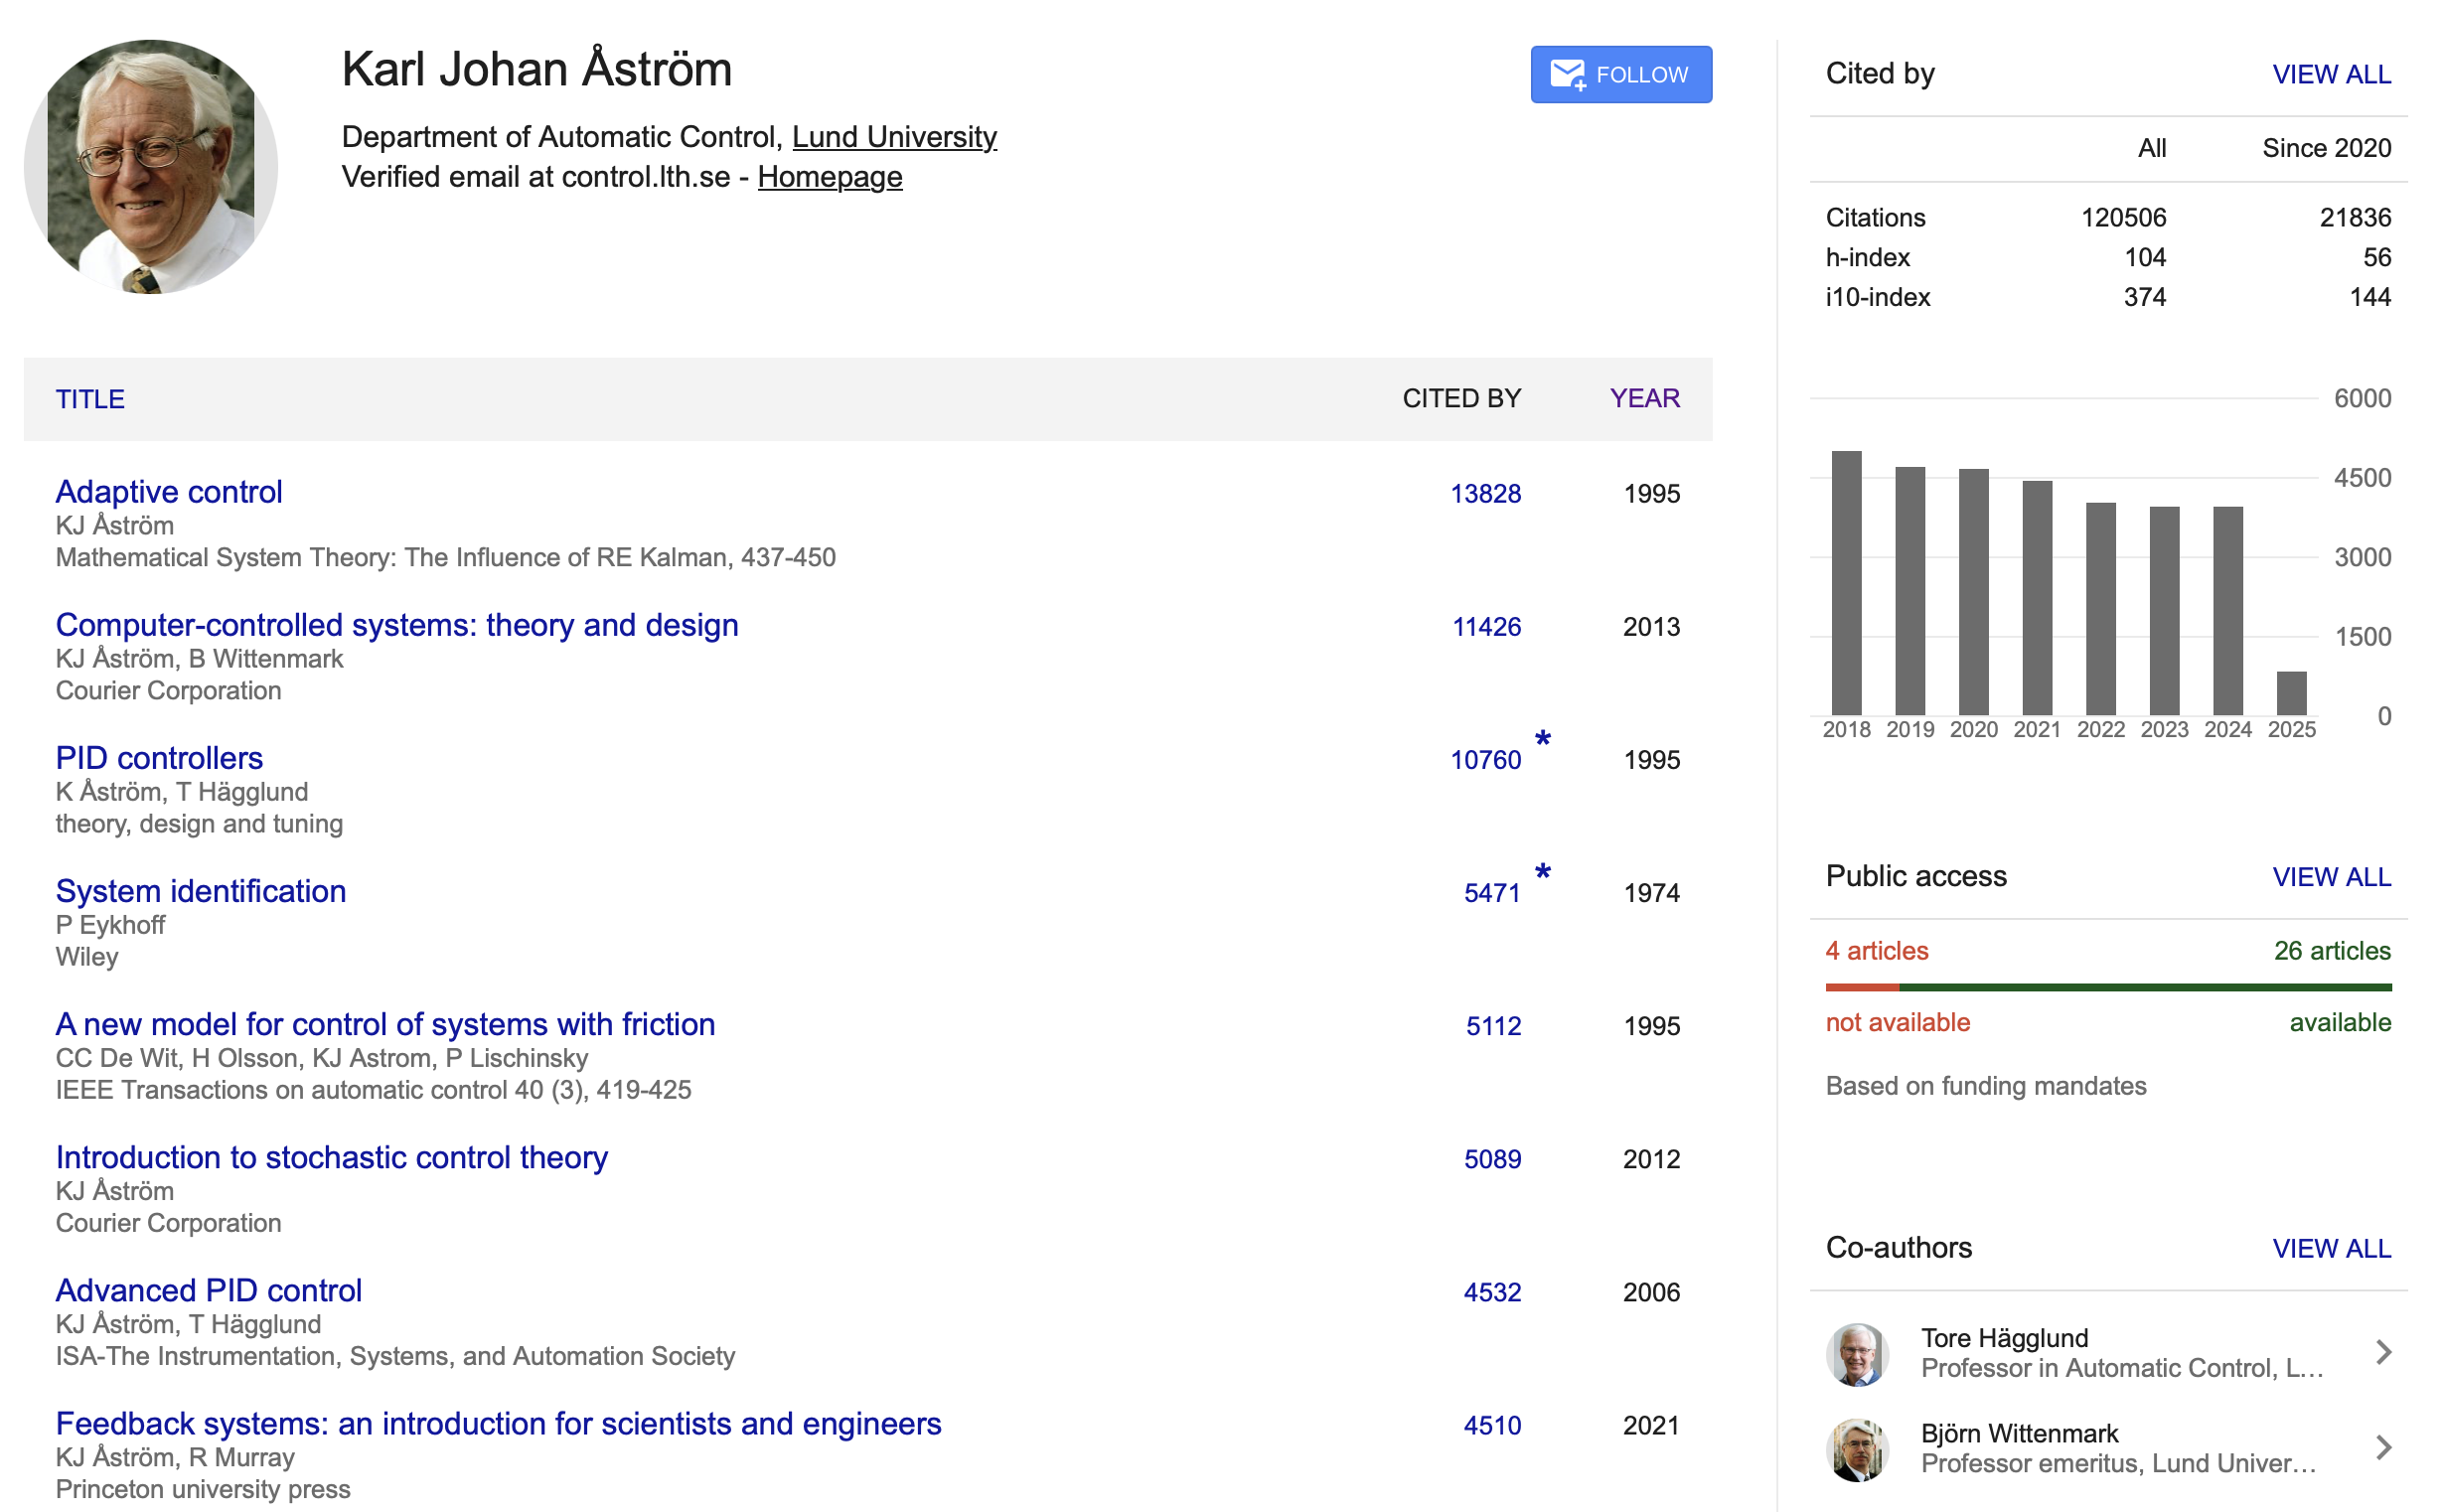
\includegraphics[width=\linewidth]{astrom}
\end{frame}

\begin{frame}
\frametitle{The course material}
\begin{itemize}[<uncover@+->]
\item Textbook: `\emph{Feedback Systems: An Introduction for Scientists and Engineers}' by Åström \& Murray, 2nd edition.
\item The textbook is perfect for our curriculum:
\begin{itemize}
\item 10 week course, omitting some technical sections
\item No assumption of a `signals and systems' background (Laplace Transforms)
\item Rigorous yet practical with many cross-disciplinary examples
\end{itemize}
\end{itemize}
\end{frame}

\begin{frame}
\frametitle{Alongside the textbook}
\begin{itemize}
\item  Additional (background?) textbook material
\item  Occasional papers/articles from the literature
\item  External online videos for alternate viewpoints
\item  Example code
\end{itemize}
\end{frame}

\begin{frame}
\frametitle{About these slides}
\begin{itemize}
\item These slides are not intended to be standalone -- rely on the textbook if in doubt
\item The slides will sometimes interpolate, extrapolate, or introduce certain elements out of place
\item You can suggest improvements to the slides here: \url{https://github.com/AUMAG/applied-control-systems}
\end{itemize}
\end{frame}

\begin{frame}
\frametitle{Course modules and topics}
\small

\centerline{%
\begin{tabular}{>{\hangindent=1em\raggedright\arraybackslash}l>{\hangindent=1em\raggedright\arraybackslash}p{5cm}l}
\toprule
Module & Topic & \S \\
\midrule
Dynamical Systems & Introduction and System Modelling & Ch.1,3 \\ 
& Dynamic Behaviour & Ch.4,5 \\ 
& Linear Systems & Ch.6 \\\midrule
Control System Concepts & State Feedback & Ch.7 \\ 
& Transfer Functions& Ch.9 \\ 
& Frequency Domain Analysis& Ch.10 \\\midrule
Control System Design & PID Control& Ch.11 \\ 
& Frequency Domain Design& Ch.12 \\ 
& Robust Performance \& Fundamental Limits& Ch.13,14  \\
\bottomrule
\end{tabular}}
\end{frame}

\FINALE

\end{document}


\MODULE{Dynamical Systems}

\TOPIC{Introduction and System Modelling}

  \documentclass{beamer-control}
\usepackage{beamer-control-singlefile}
\INCLUDEONLY{Introduction}
\begin{document}
\CONCEPT{Introduction}

\begin{SUMMARY}
\begin{itemize}
\item What is a Dynamical System?
\item What is Feedback and Feedforward?
\item What is Control?
\item Feedback Properties (or `why control?')
\item Simple Forms of Feedback
\item Broader Concepts of Control
\end{itemize}
\vfill References:
\begin{itemize}
\item \astrom{Chapter 1}
\item \url{https://engineeringmedia.com/map-of-control}
\end{itemize}
\end{SUMMARY}

\begin{frame}
\frametitle{What is a Dynamical System?}

Dynamical systems have variables (or \emph{states}) $\mathbf{x}$ which change over time:
\begin{align}
\dot \mathbf{x}(t) = f(\mathbf{x},t)
\end{align}
They generally do not exist alone, and include inputs $\mathbf{u}$:
\begin{align}
\dot \mathbf{x}(t) = f(\mathbf{x},t) + \mathbf{u}(t)
\end{align}
Dynamical systems can be linear or nonlinear, solvable analytically or only numerically.

\bigskip
\uncover<2>{\emph{\alert{We must understand dynamical systems before control systems.}}}
\end{frame}

\begin{frame}{What is Feedback? \AMref{§1.1}}
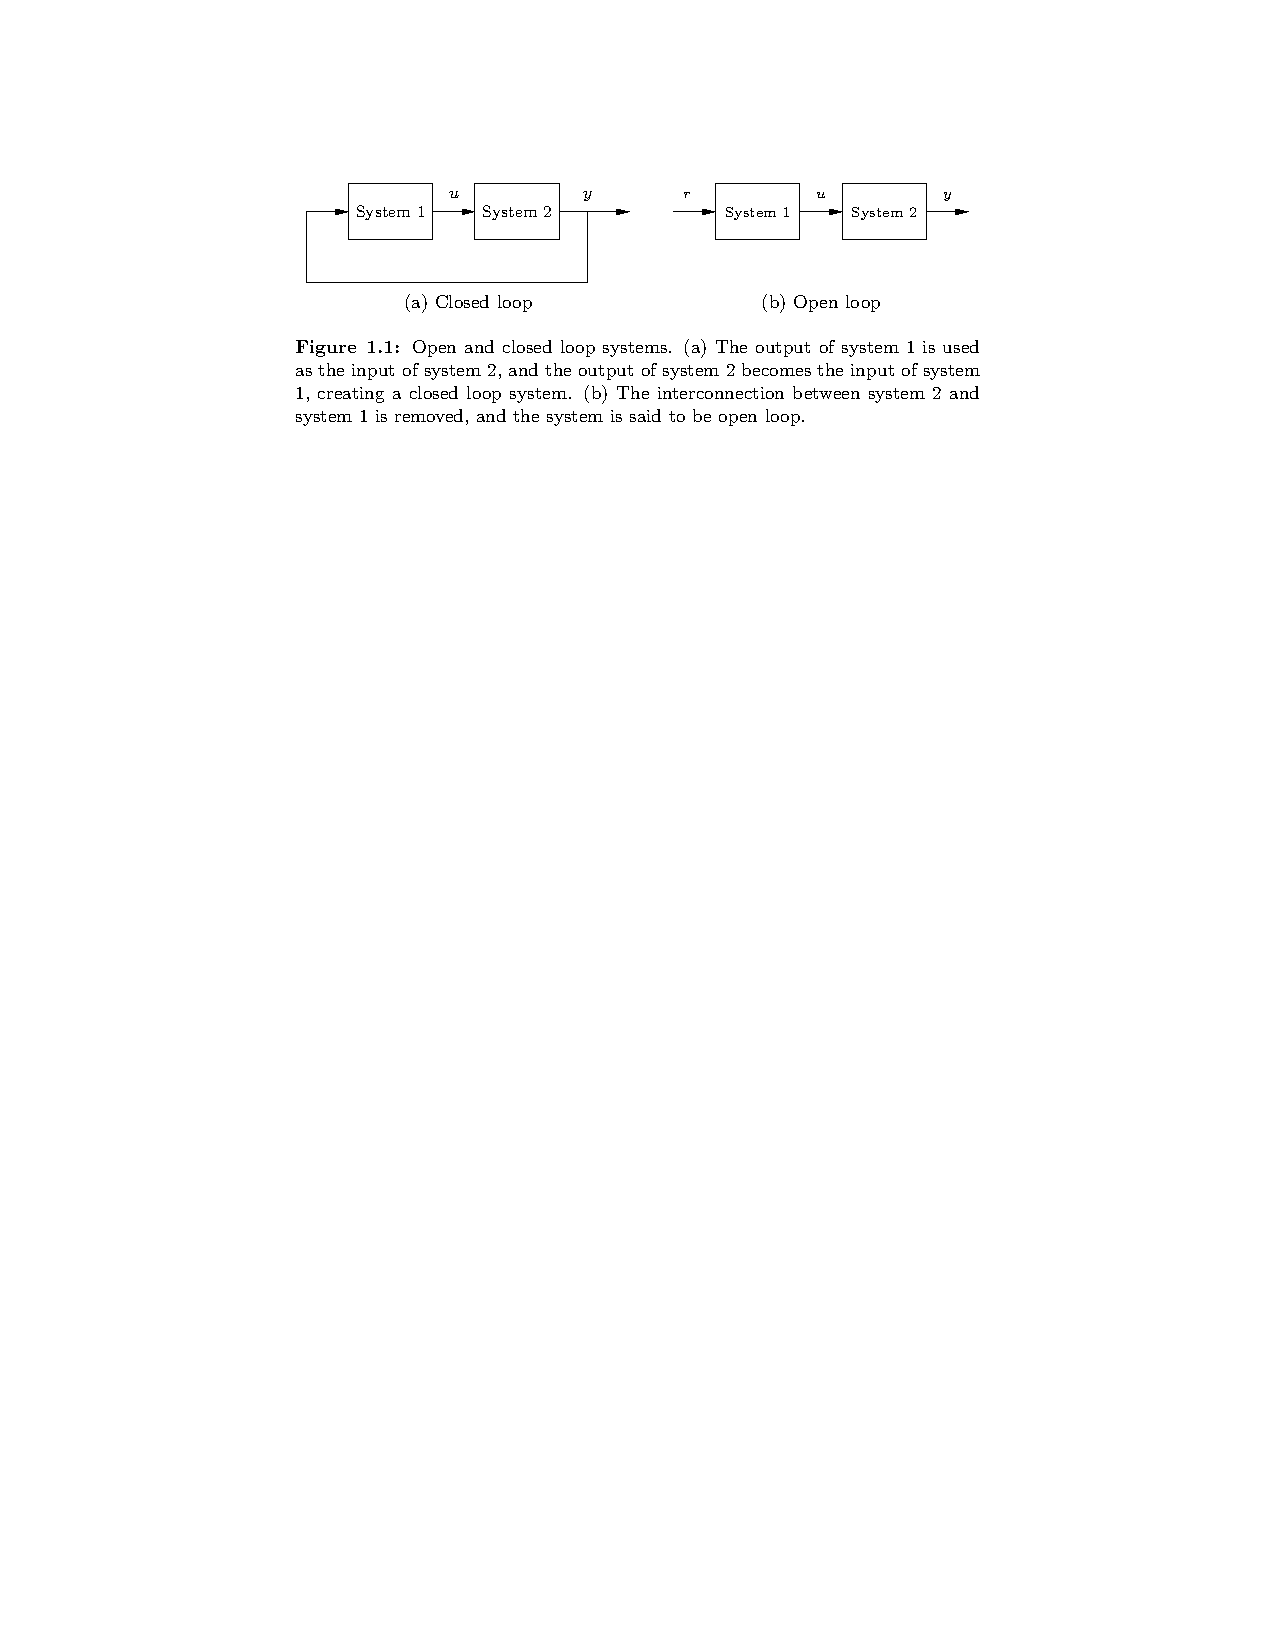
\includegraphics[width=\linewidth]{figure1.1}
\end{frame}

\begin{frame}{What is Feedforward? \AMref{§1.2}}
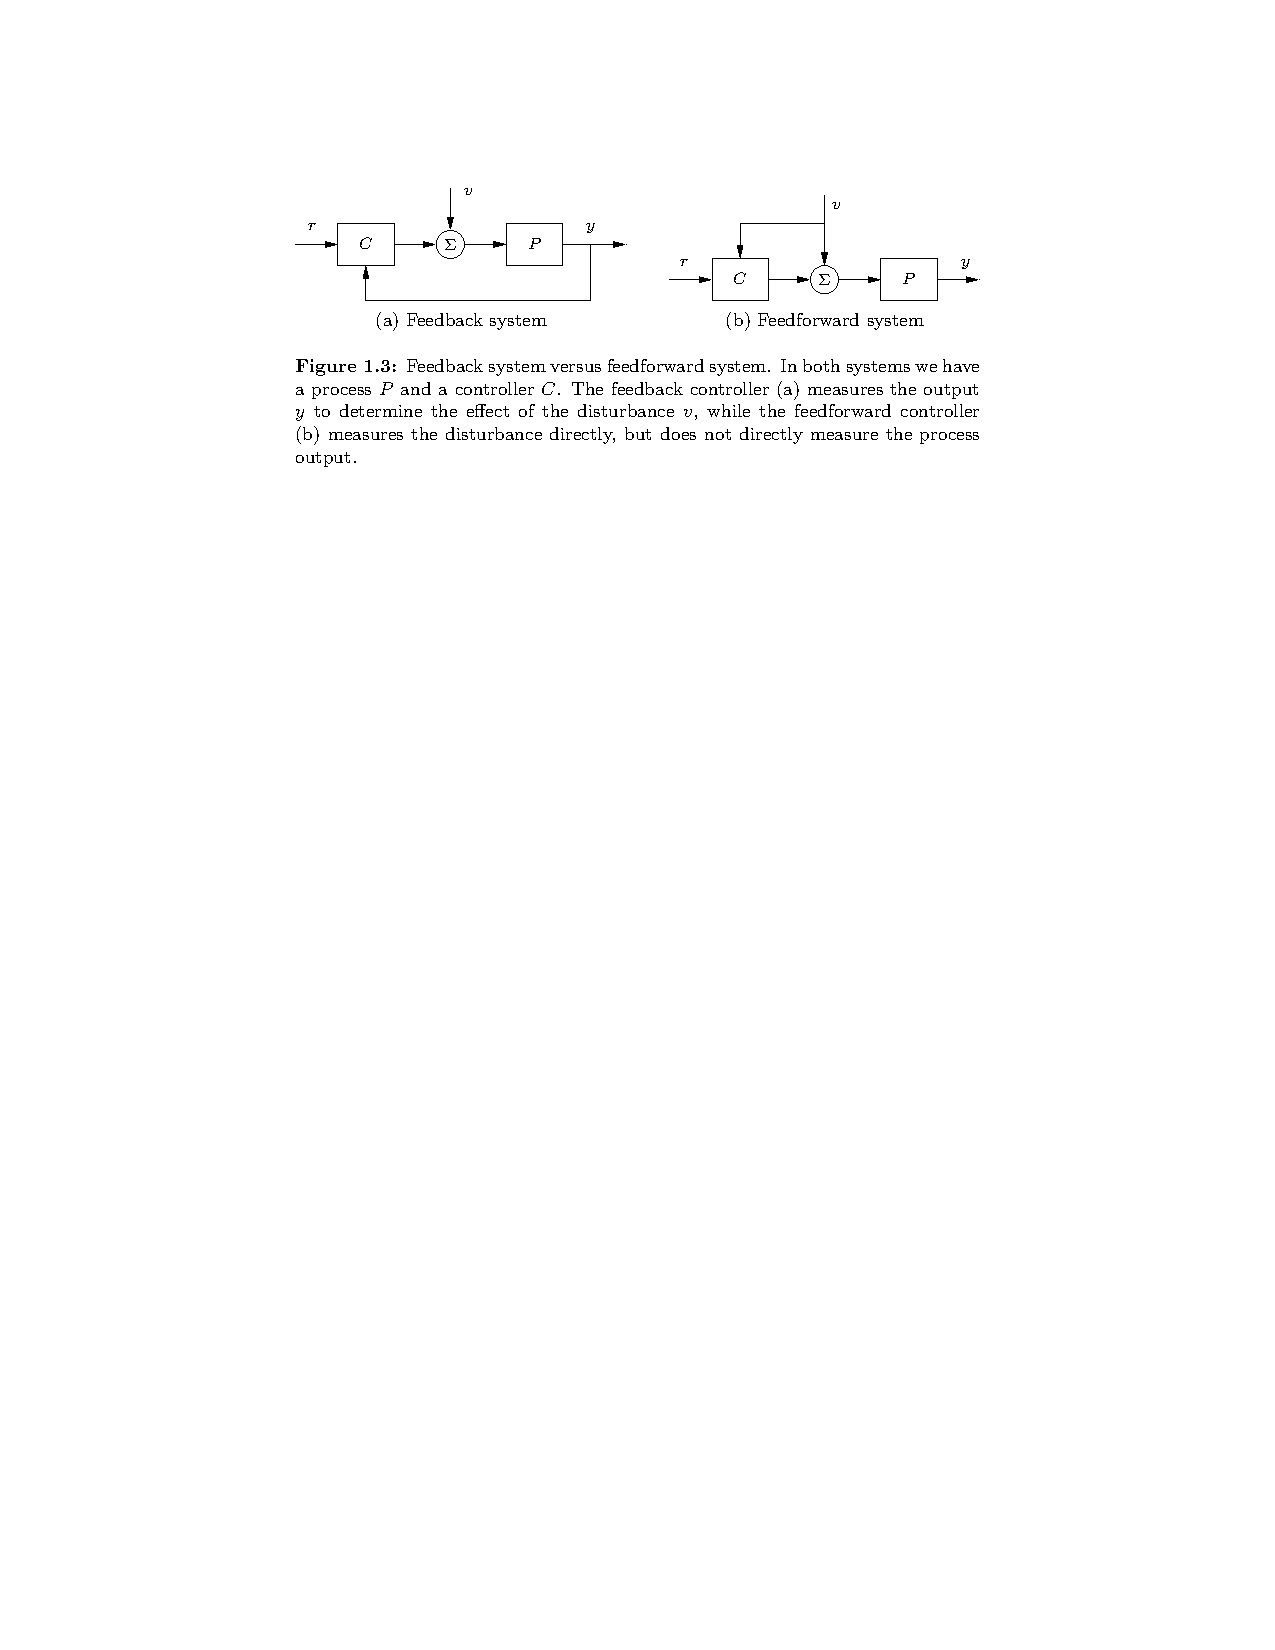
\includegraphics[width=\linewidth]{figure1.3}
\end{frame}

\begin{frame}{What is Control? \AMref{§1.3}}
Augmenting a system to change/improve its dynamics:
\begin{itemize}
\item Passive control: adding a passive element (usually trivial)
\item Active control: adding a feedback (or feedforward) loop
\item Generally involves three elements:
\begin{itemize}
\item Sensors (can't control what you don't know)
\item Controller (calculate what to do based on the state)
\item Actuators (effect the desired changed)
\end{itemize}
\end{itemize}
\end{frame}

\begin{frame}
\frametitle{The cruise control feedback system}

\end{frame}

\begin{frame}{Uses of Feedback and Control \AMref{§1.4}}
Control systems are truly multidisciplinary:
\begin{itemize}
\item Power systems (Elec Eng)
\item Process systems (Chem Eng)
\item Aerospace systems (Mech Eng)
\item Infrastructure systems (Civil/Environ Eng)
\item Economics (tariffs!)
\item Biology, Ecology, Climate Change \dots
\end{itemize}
\end{frame}

\begin{frame}
\frametitle{Feedback Properties \AMref{§1.5}}
\begin{itemize}
\item<only@1> General solution to asking an engineering system to respond to demands
\item<only@2> Robustness to uncertainty
\begin{itemize}
\item Rejection of disturbances
\item Mitigating sources of error
\item Adapting to changing conditions
\end{itemize}
\item<only@3> Design of dynamics
\begin{itemize}
\item Controlling stability (aerospace)
\item Precise control (robotics)
\end{itemize}
\item<only@4> Challenges
\begin{itemize}
\item Stability
\item Coupling
\item Complexity
\end{itemize}
\end{itemize}
\end{frame}


\begin{frame}
\frametitle{The canonical control block diagram}

\end{frame}


\begin{frame}
\frametitle{Simple Forms of Feedback \AMref{§1.6}}
\framesubtitle{On-Off Control}
\fbox{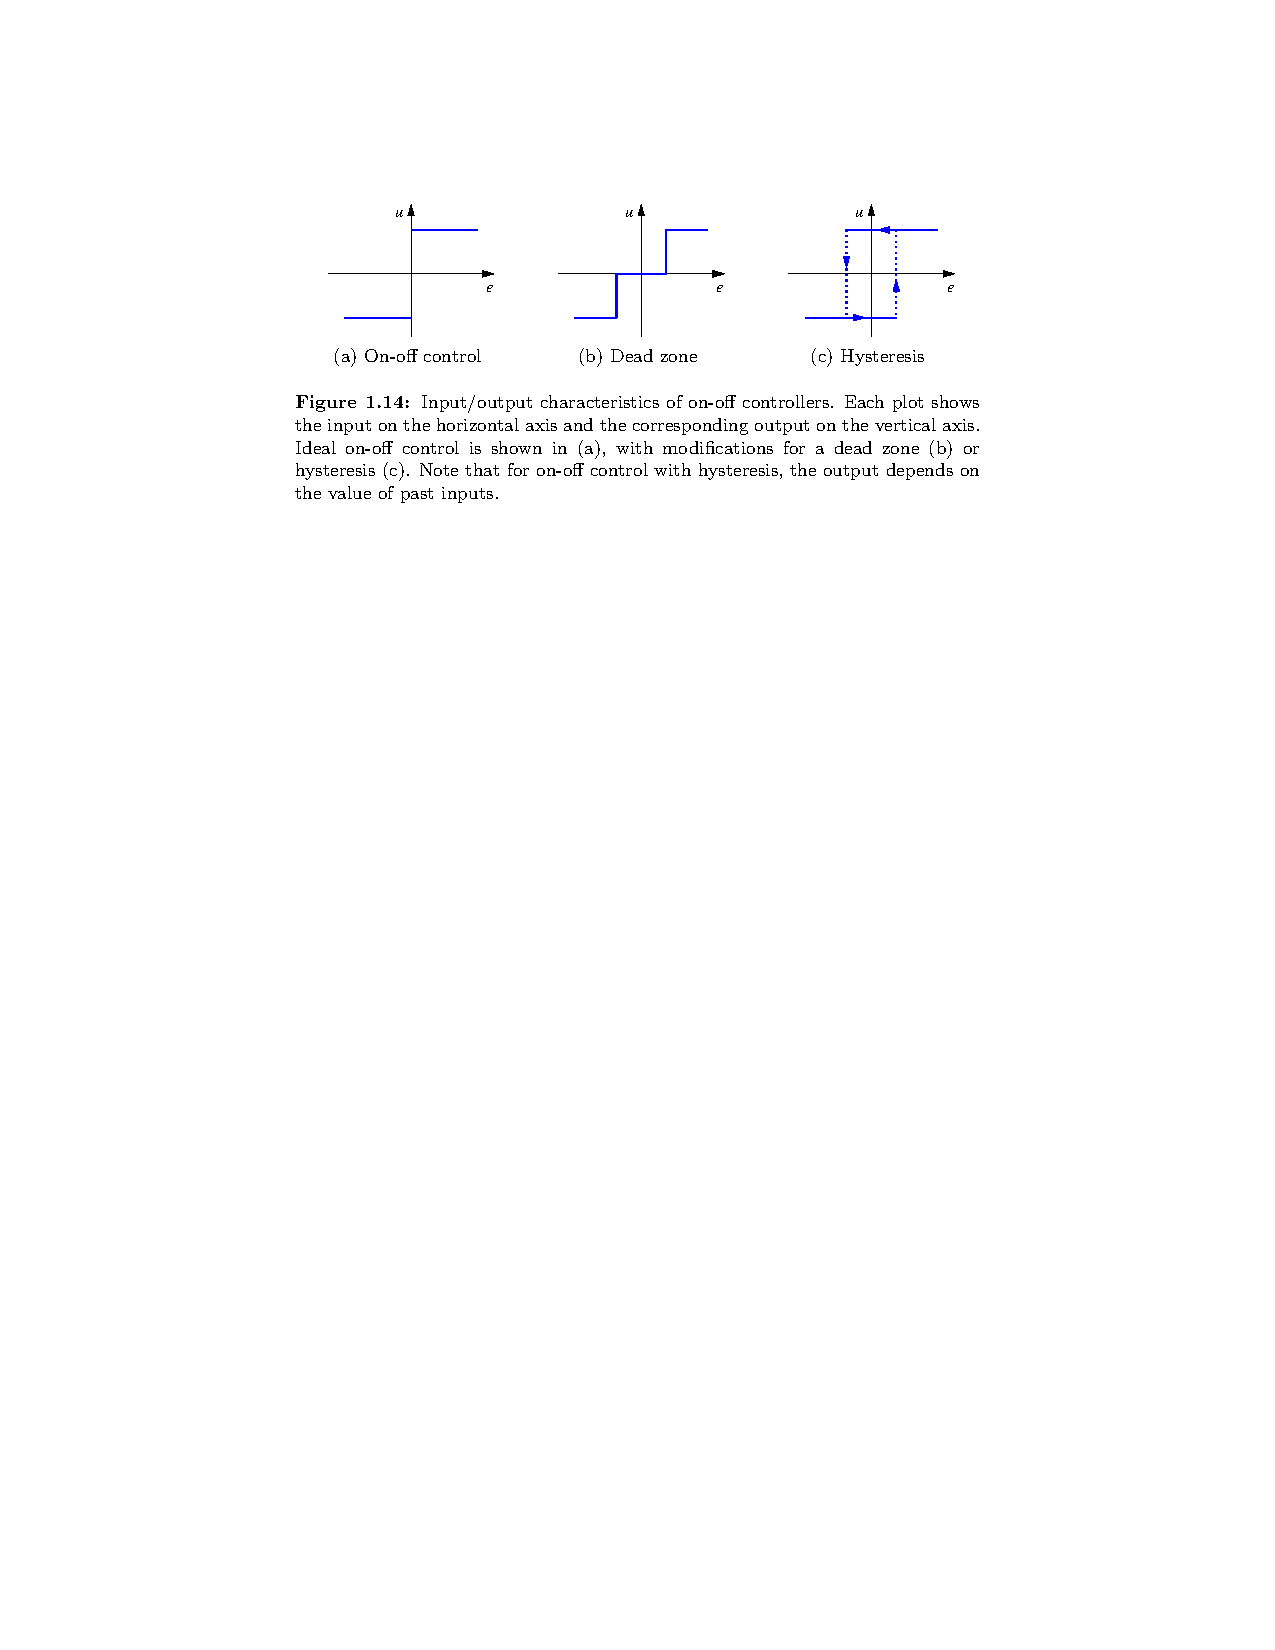
\includegraphics[width=\linewidth,trim=0 41 0 0,clip]{figure1.14}}
\begin{gather}
u(t) = \operatorfont{sign}(e)\, u_{\mathrm{max}}
\end{gather}
\end{frame}

\begin{frame}
\frametitle{Simple Forms of Feedback \AMref{§1.6}}
\framesubtitle{PID Control}
\fbox{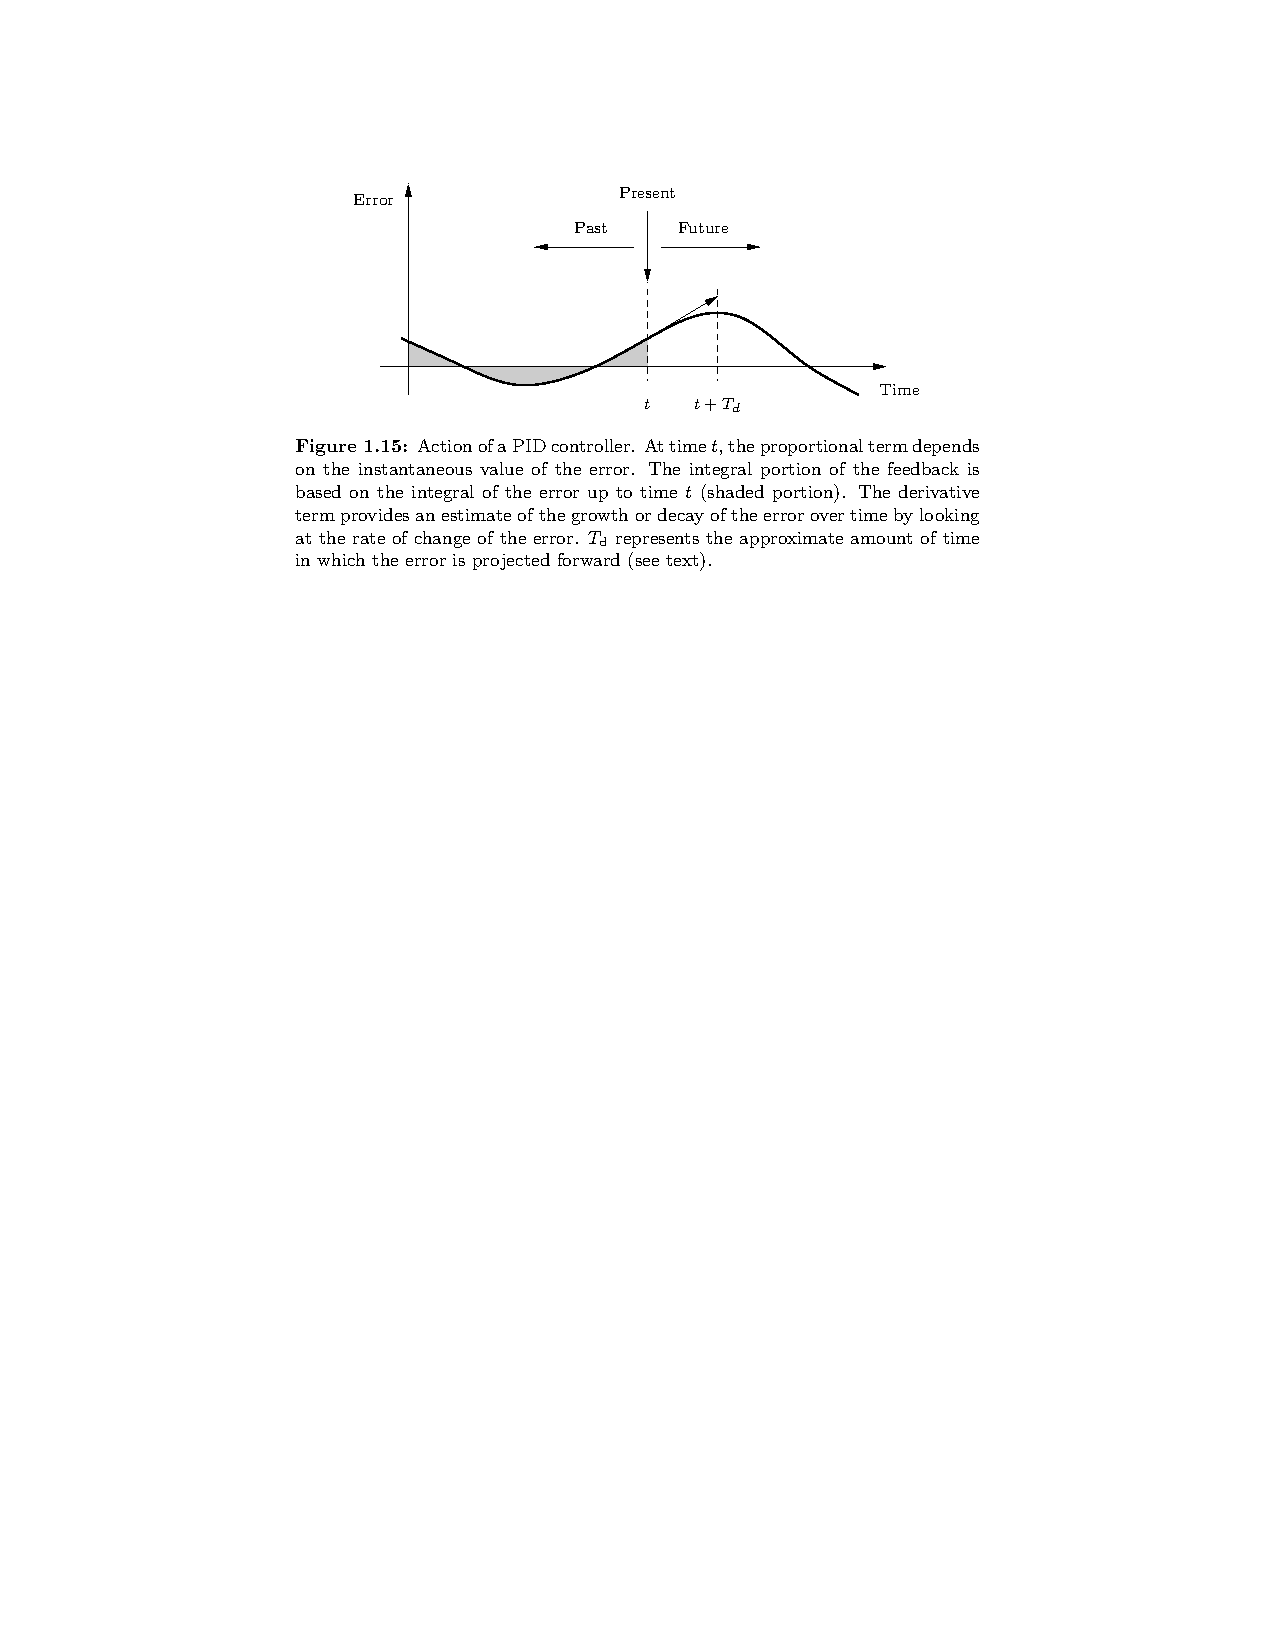
\includegraphics[width=\linewidth,trim=0 52 0 0,clip]{figure1.15}}
\vfil
\begin{gather}
u(t) = k_p e(t) + k_i \int_0^t e(\tau) \mathrm d\tau + k_d \frac{\mathrm d e(t)}{\mathrm d t}
\end{gather}
\end{frame}

\begin{frame}
\frametitle{Combining Feedback with Logic \AMref{§1.7}}
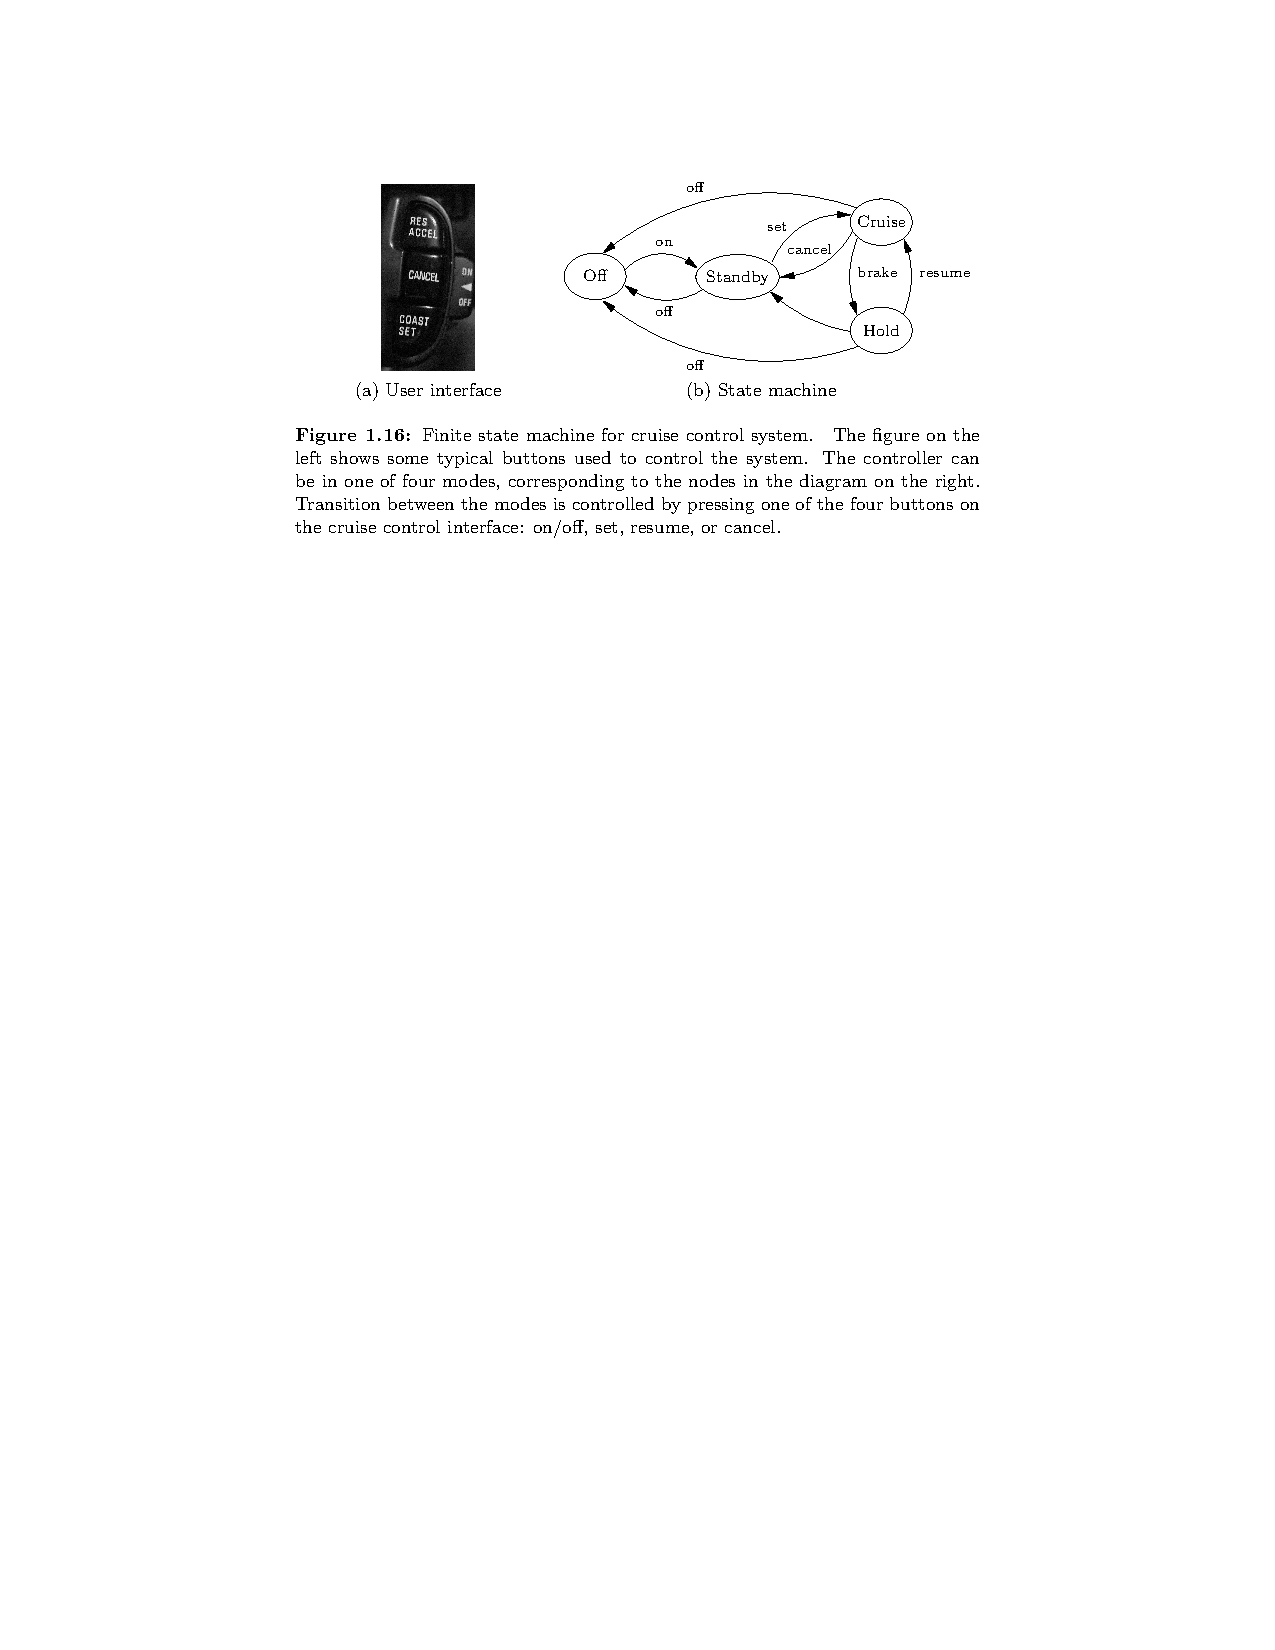
\includegraphics[width=\linewidth]{figure1.16}
\end{frame}

\begin{frame}
\frametitle{Control System Architectures \AMref{§1.8}}
\centering
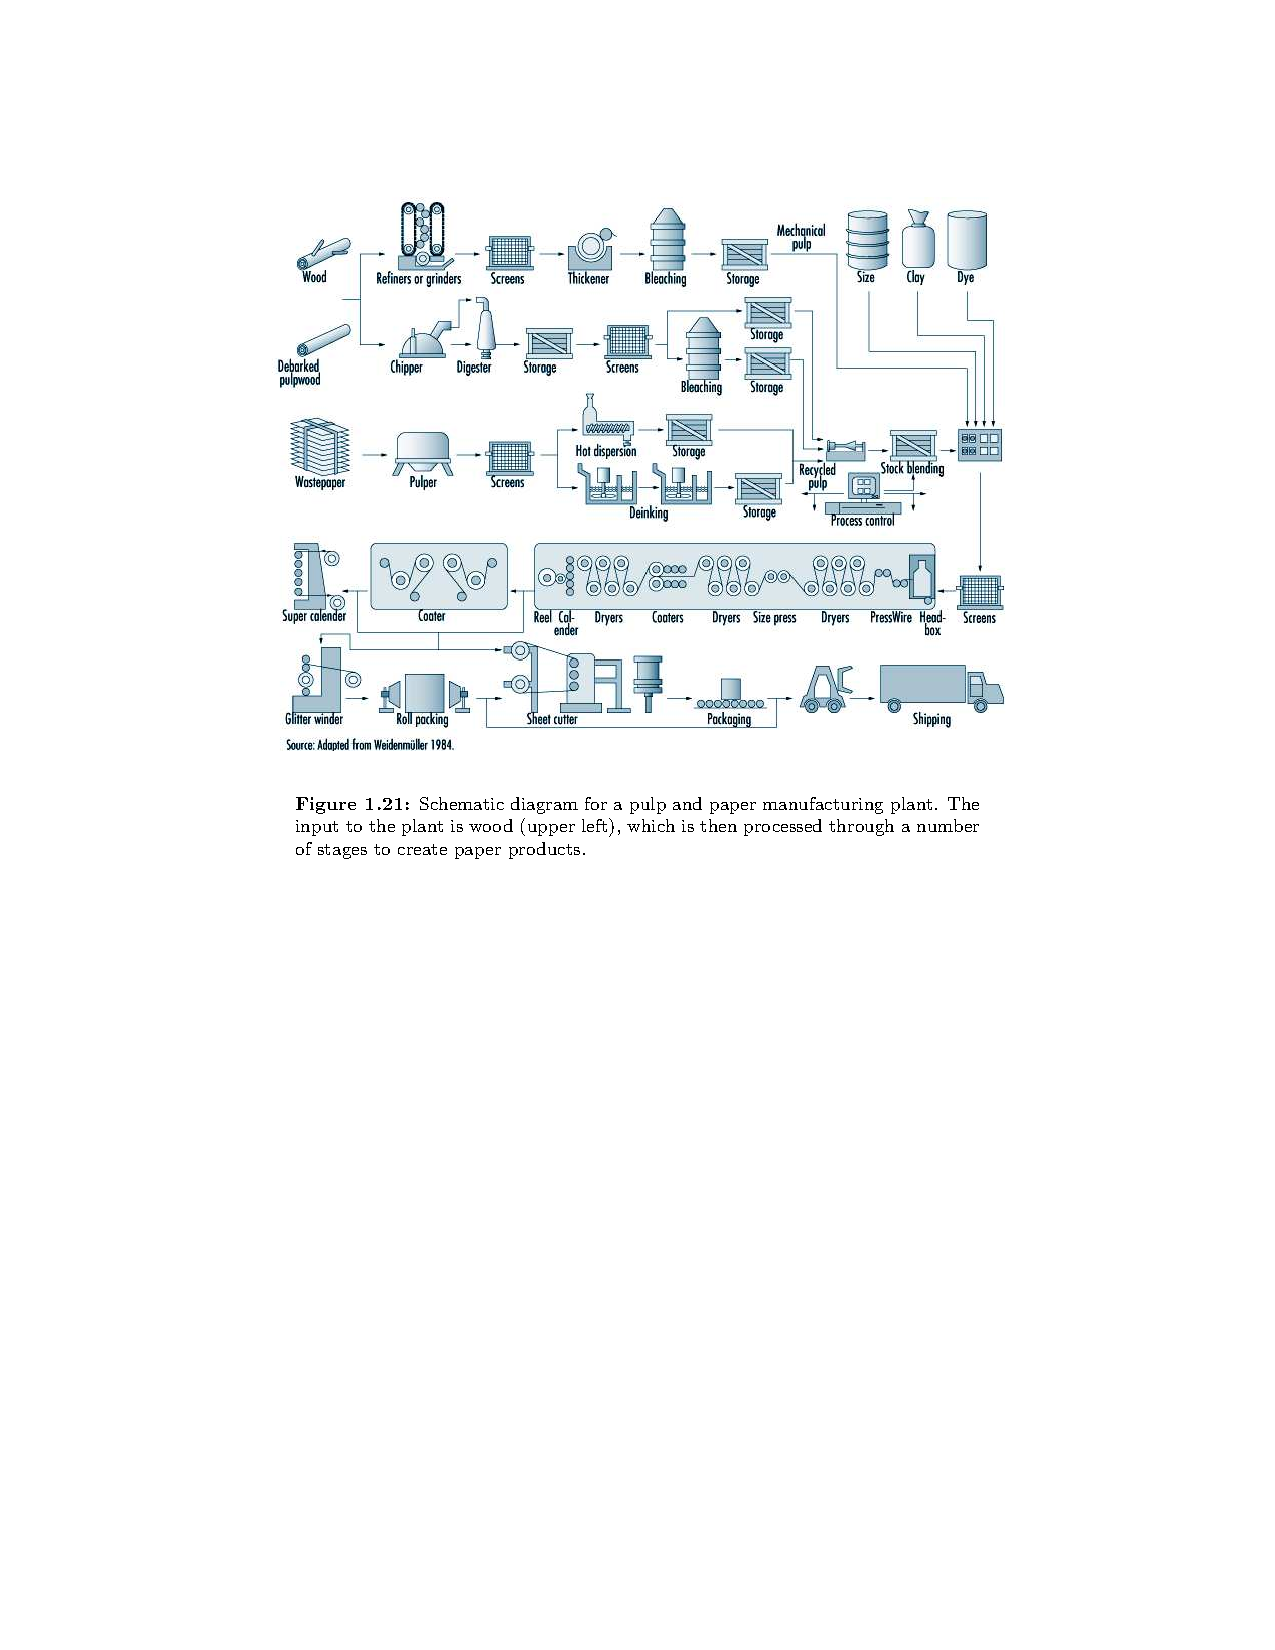
\includegraphics[width=0.8\linewidth]{figure1.21}
\end{frame}

\begin{frame}
\frametitle{Brian Douglas' Map of Control Theory}
\centering
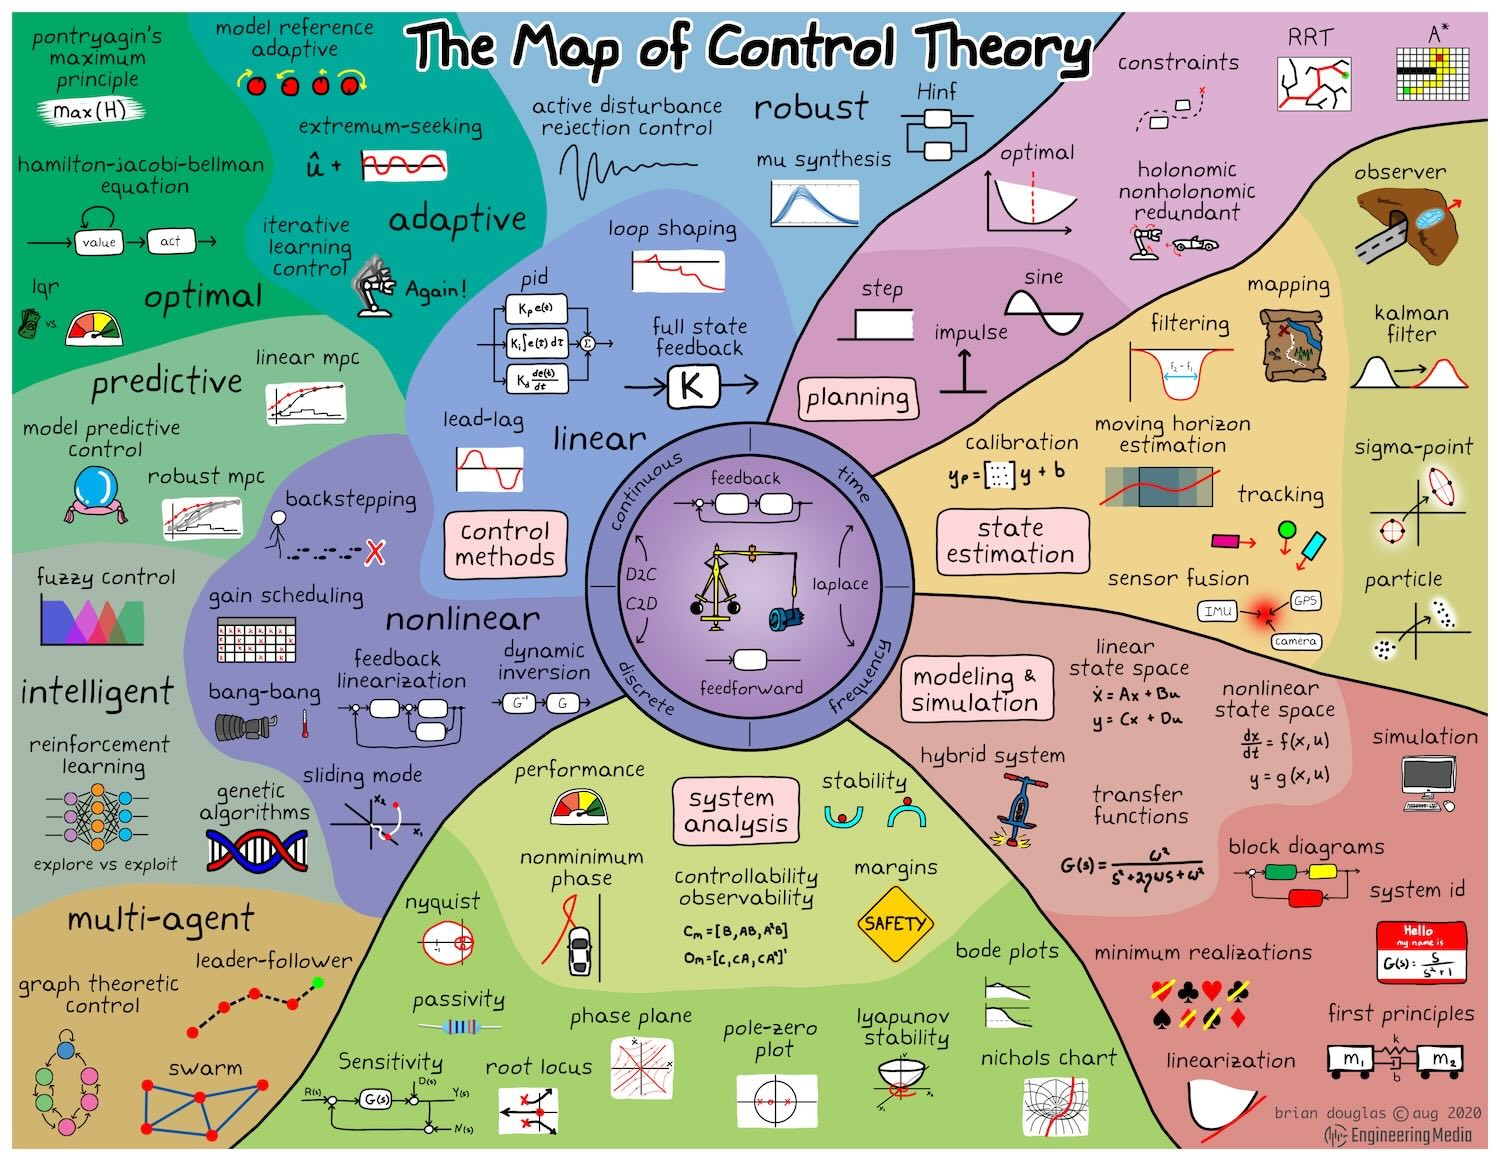
\includegraphics[width=0.90\linewidth]{Control_Map_ver5_wr}
\end{frame}

\SUMMARYFRAME
\FINALE

\end{document}

  \documentclass{beamer-control}
\usepackage{beamer-control-singlefile}
\INCLUDEONLY{Modeling Concepts}
\begin{document}
\CONCEPT{Modeling Concepts}

\begin{SUMMARY}
\begin{itemize}
\item Systems, models
\item Variables, states, `state space'
\item Example of nonlinear model output
\item Example of linear time-invariant model output
\item Standard control equation
\end{itemize}
\vfill References:
\begin{itemize}
\item \astrom{§3.1}
\end{itemize}
\end{SUMMARY}


\begin{frame}{Systems and models}

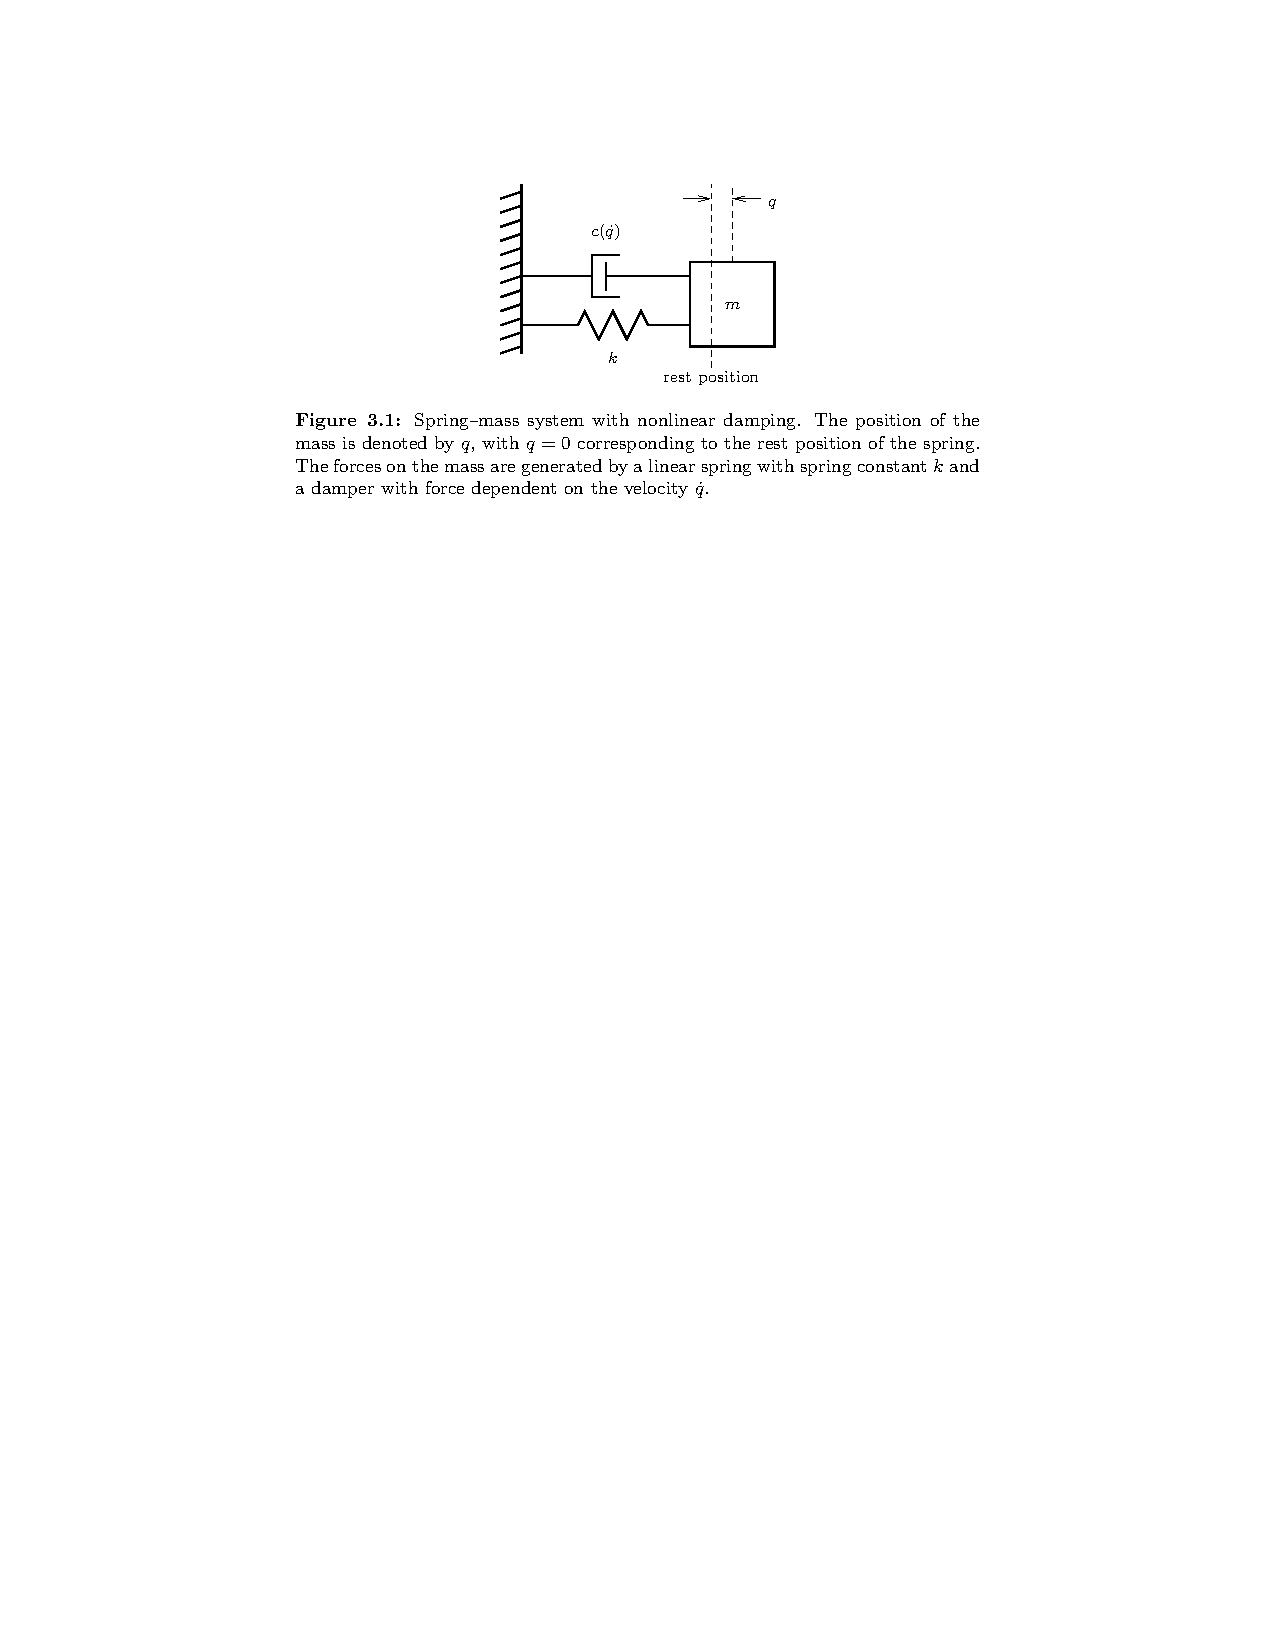
\includegraphics[width=\linewidth]{figure3.1}

\end{frame}

\begin{frame}
\frametitle{State model --- mass-spring-damper with nonlinear damping}

\vspace*{-5mm}
\begin{align}
m \ddot q + c(\dot q) + kq &= 0 & x &= \Matr{q\\ \dot q}
\end{align}

\centering
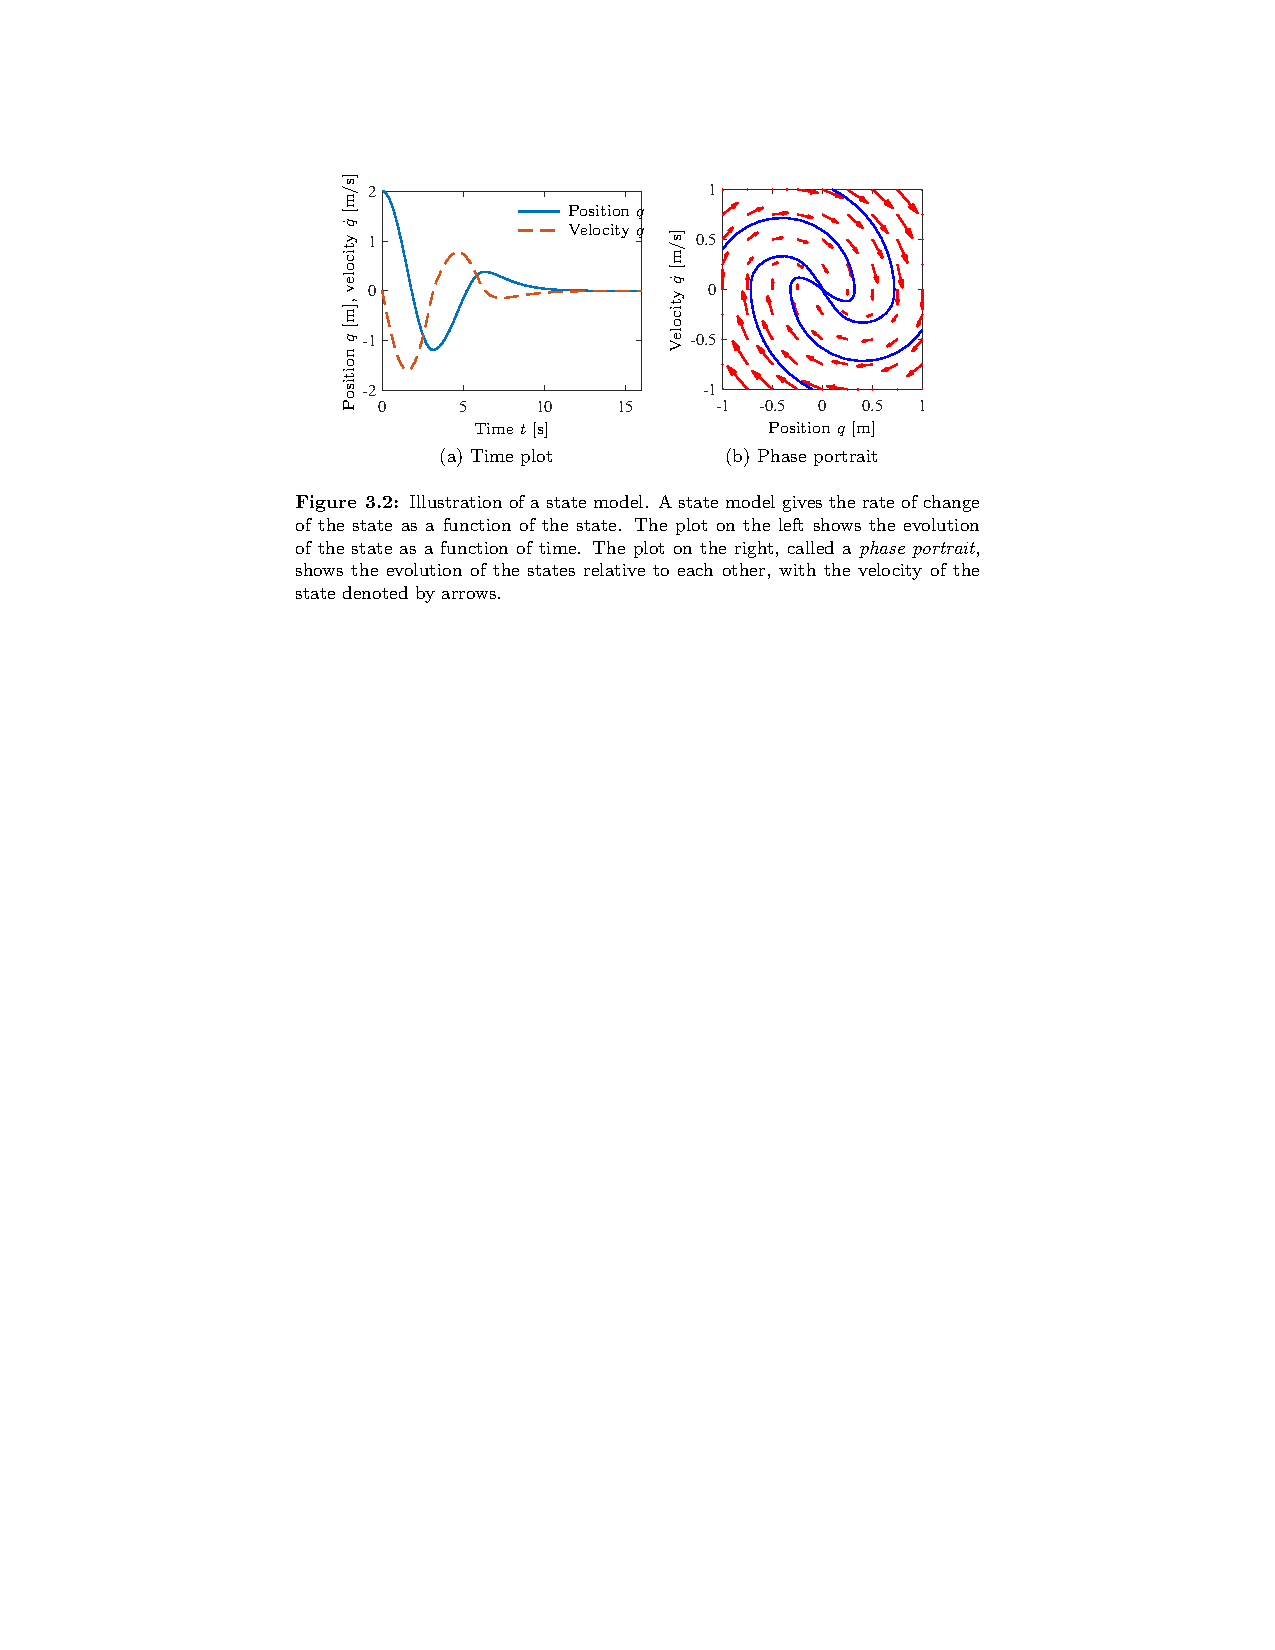
\includegraphics[width=0.9\linewidth]{figure3.2}

\end{frame}

\begin{frame}
\frametitle{Input-output models}
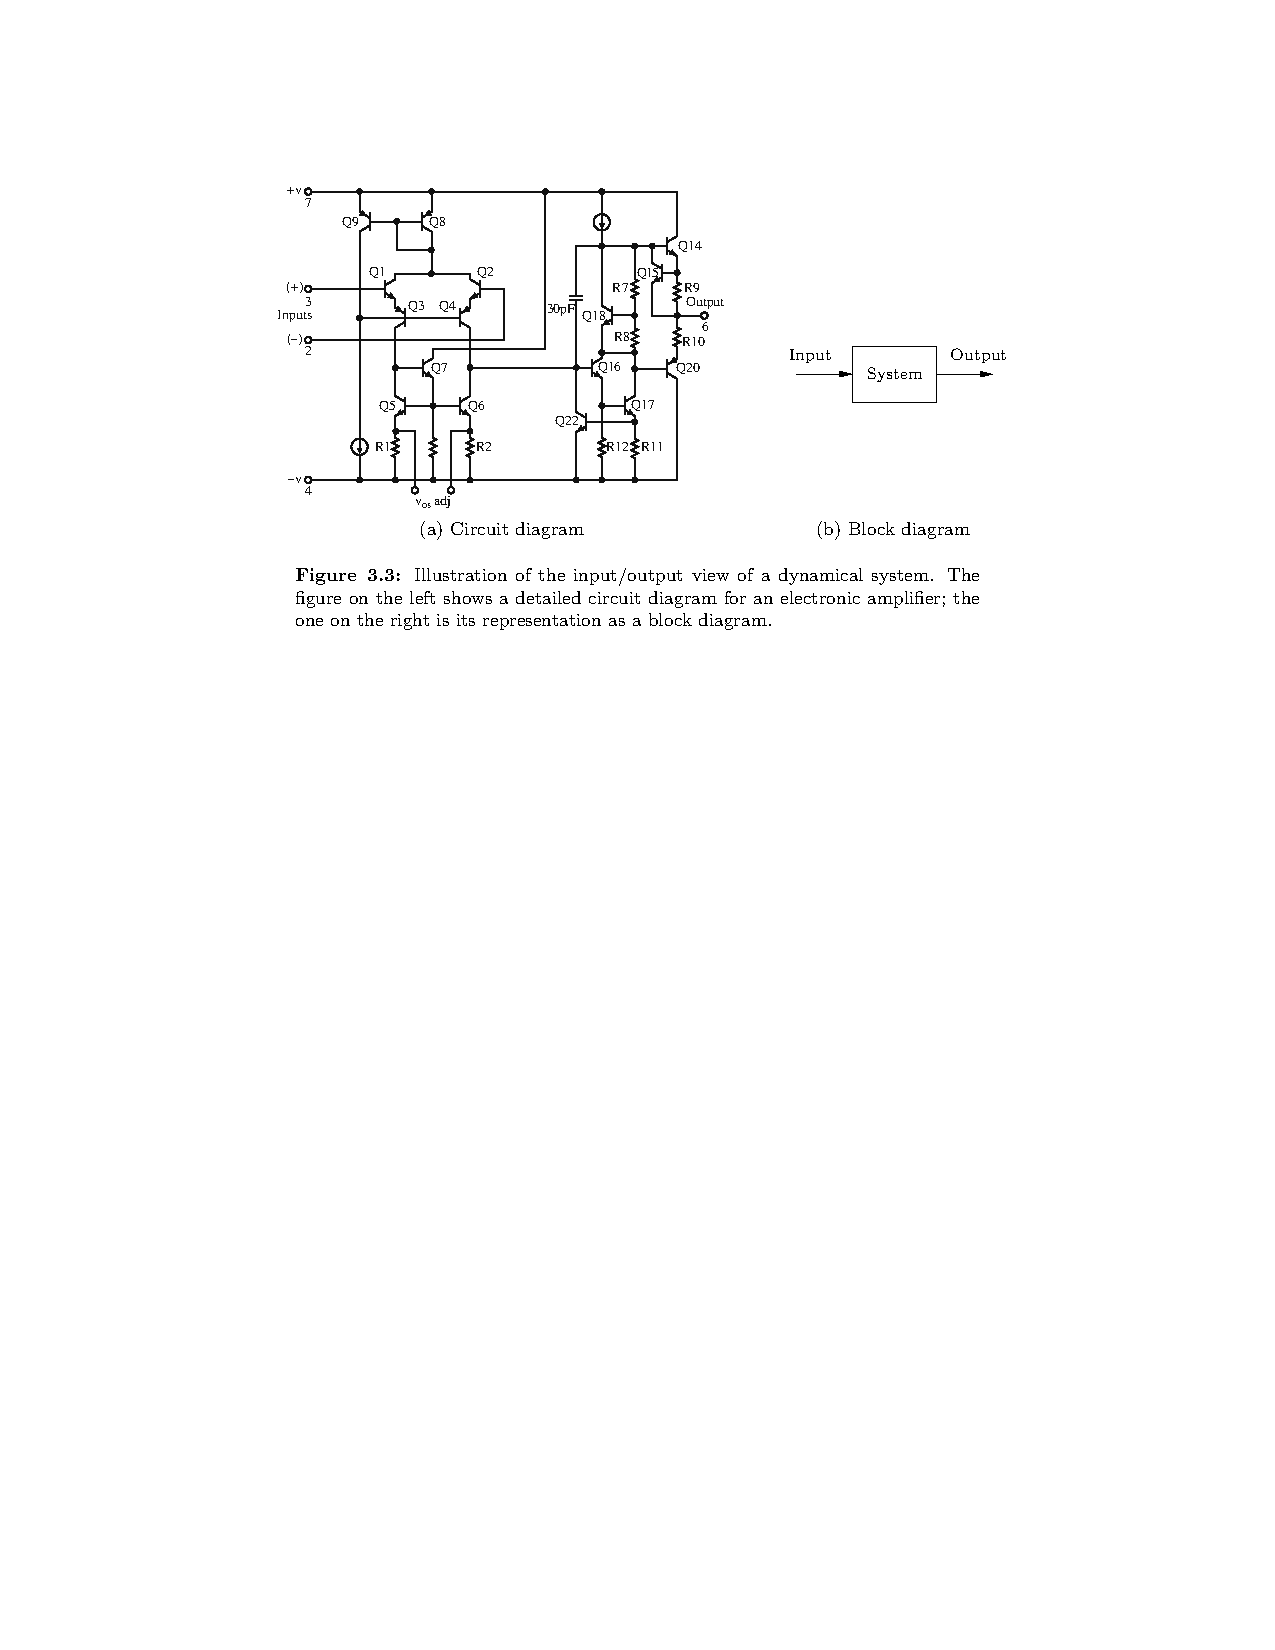
\includegraphics[width=\linewidth]{figure3.3}
\end{frame}

\begin{frame}
\frametitle{Linear time-invariant models}
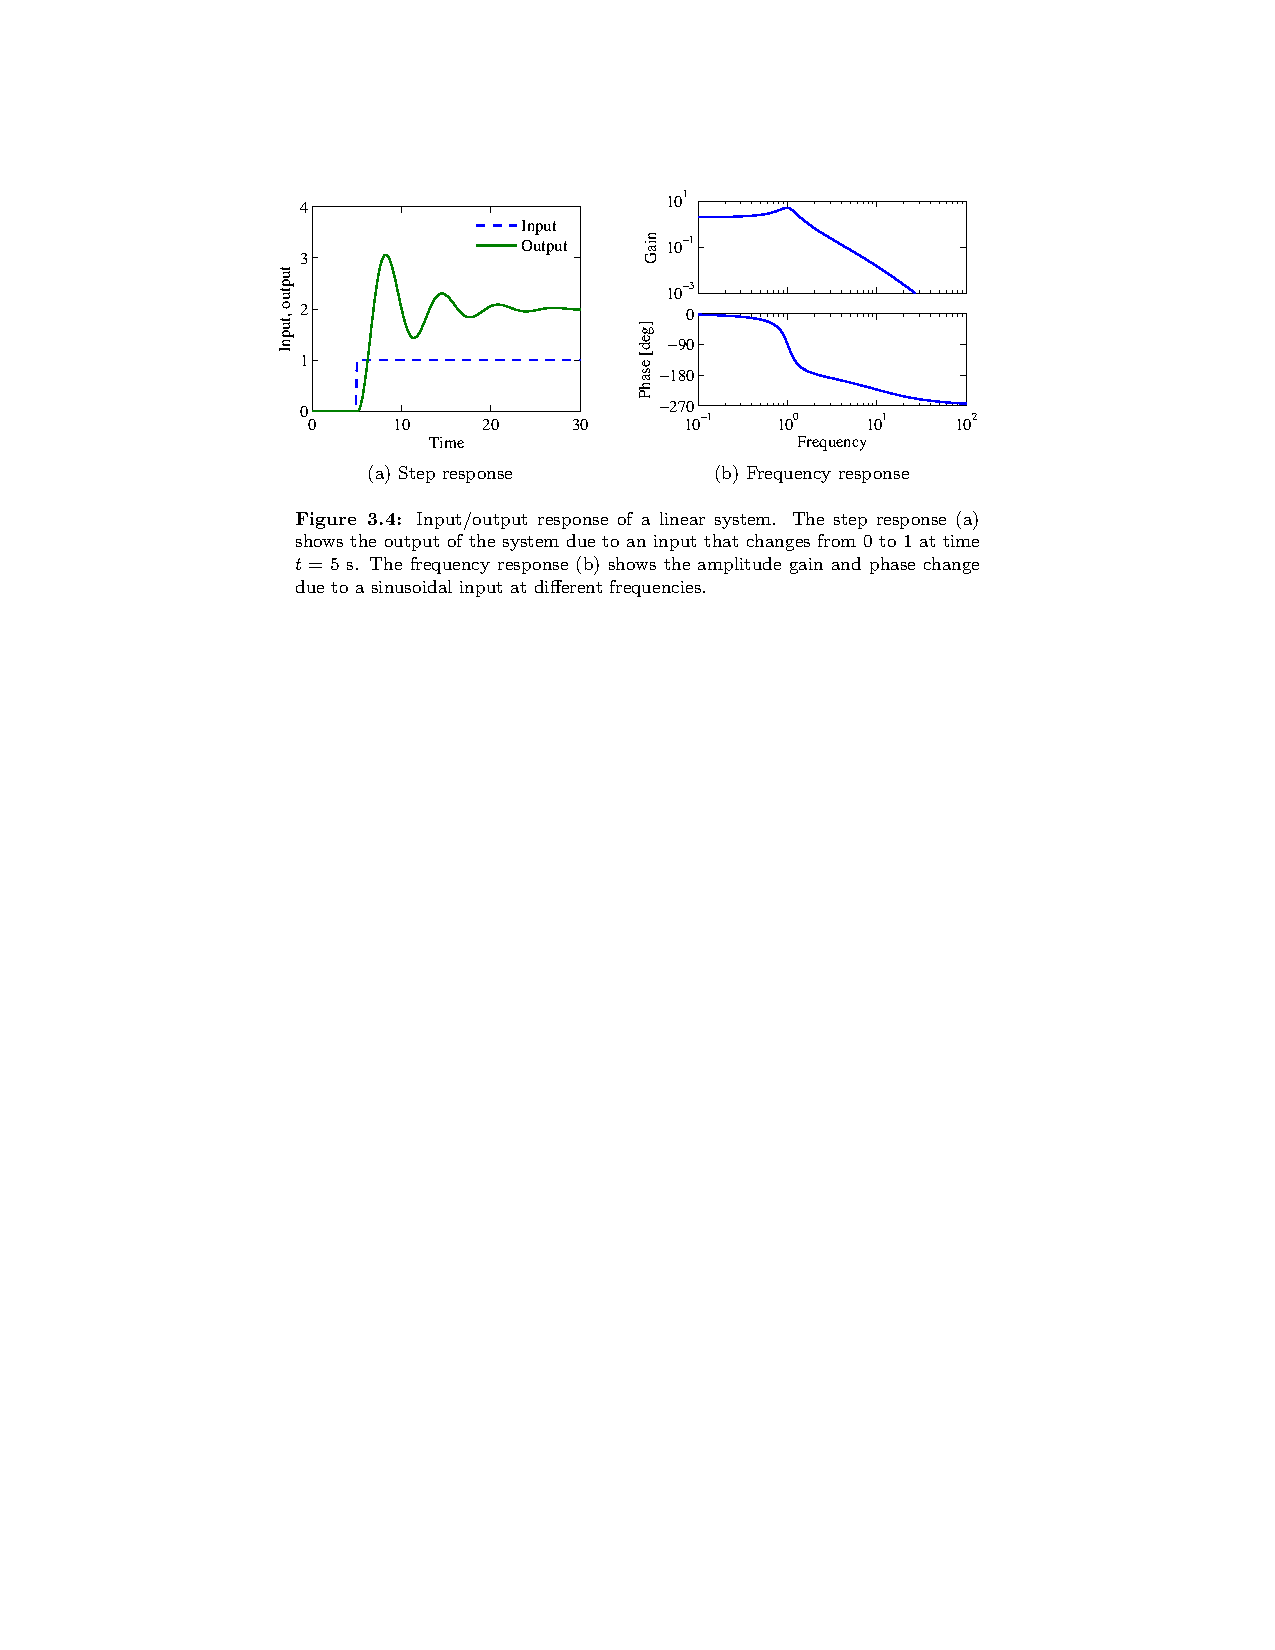
\includegraphics[width=\linewidth]{figure3.4}
\end{frame}

\begin{frame}
\frametitle{Standard nonlinear control equation}
\begin{align}
\Deriv{x}{t} &= f(x,u) & y &= h(x,u)
\end{align}
Recall nonlinear spring example with $x = [q\quad \dot q]\Tr$:
\begin{align}
\Deriv{x}{t} &= \begin{bmatrix}\dot q\\\ddot q\end{bmatrix} = \begin{bmatrix}\dot q\\- c(\dot q)/m - kq/m\end{bmatrix}
\end{align}
If we measure displacement $q$:
\begin{align}
y = h(x,u) &= q
\end{align}
Use these equations to simulate, simplify, analyse\dots

\end{frame}



\SUMMARYFRAME
\FINALE

\end{document}

  \documentclass{beamer-control}
\usepackage{beamer-control-singlefile}
\INCLUDEONLY{State Space Models}
\begin{document}
\CONCEPT{State Space Models}

\begin{SUMMARY}
\begin{itemize}
\item Ordinary Differential Equations
\item Difference Equations
\item Simulation and Analysis
\end{itemize}
\vfill References:
\begin{itemize}
\item \astrom{§3.2}
\end{itemize}
\end{SUMMARY}


\begin{frame}
\frametitle{Terminology}
\begin{itemize}
\item What is a state variable?
\item What is an input?
\item What is an output?
\item What is `dynamics'?
\end{itemize}
\end{frame}

\SUBCONCEPT{Ordinary Differential Equations}

\begin{frame}
\frametitle{State space model}
We have already written this down:
\begin{align}
\Deriv{x}{t} &= f(x,u) & y &= h(x,u)
\end{align}
$x$ is the state vector which contains the state variables, e.g.:
\begin{align}
x = \begin{bmatrix} x_1 \\ x_2 \\ \dot x_1 \\ \dot x_2 \end{bmatrix}
\end{align}
In this example, $x$ is the state vector for an order 4 system.
\end{frame}

\begin{frame}
\frametitle{Linear state space model}
We commonly model state space systems as being `linear time invariant' (LTI).
In the previous concept, we wrote:
\begin{align}
\dot x &= \begin{bmatrix}\dot q\\\ddot q\end{bmatrix} = \begin{bmatrix}\dot q\\- c(\dot q)/m - kq/m\end{bmatrix}
\end{align}
Let's now linearise with $c(\dot q) \eqdef c q$:
\begin{align}
\dot x &= \begin{bmatrix}\dot q\\\ddot q\end{bmatrix} = \begin{bmatrix}\dot q\\- cq/m - kq/m\end{bmatrix} 
              = \begin{bmatrix}0 & 1\\- c/m & - k/m\end{bmatrix}\begin{bmatrix} q\\\dot q\end{bmatrix} = Ax
\end{align}
\end{frame}

\begin{frame}
\frametitle{Linear state space equations}
\begin{align}
\dot x &= Ax + Bu & y &= Cx + Du
\end{align}
E.g., if we added an input force to the mass-spring-damper:
\begin{align}
m\ddot q + c\dot q + kq = f
\end{align}
The $Ax$ term is the same, and:
\begin{align}
Bu = \begin{bmatrix} 0\\ 1/m\end{bmatrix}\begin{bmatrix} f\end{bmatrix} = \begin{bmatrix} 0\\ f/m\end{bmatrix}
\end{align}
\QUIZ{Å\&M have a different formulation for $x$ -- is either more correct?}
\end{frame}

\begin{frame}
\frametitle{Now Å\&M throw you in the deep end\dots}
General mechanical dynamics:
\begin{align}
\underbrace{M(q)}_{\text{\tiny inertia matrix}}\ddot q + \underbrace{C(q,\dot q)}_{\text{\tiny coriolis, damping}} + \underbrace{K(q)}_{\text{\tiny potential}} = \underbrace{B(q)u}_{\text{\tiny external}}
\end{align}
`Then it can be shown that' for a Segway-style system:
\begin{equation}
\begin{bmatrix}
(M + m) & -ml \cos\theta \\
-ml \cos\theta & (J + ml^2)
\end{bmatrix}
\begin{bmatrix}
\ddot{q} \\
\ddot{\theta}
\end{bmatrix}
+
\begin{bmatrix}
c\dot{q} + ml \sin\theta\, \dot{\theta}^2 \\
\gamma \dot{\theta} - mgl \sin\theta
\end{bmatrix}
=
\begin{bmatrix}
F \\
0
\end{bmatrix}
\label{eq:segway}
\end{equation}
\end{frame}


\begin{frame}
\frametitle{Banjo music\dots}
Defining some shorthands:
\begin{align}
M_t &= M+m & J_t&=J+ml^2 & c_\theta&=\cos\theta & s_\theta &= \cos\theta
\end{align}
Equation \eqref{segway} becomes:
\begin{equation}
\Deriv{}{t}
\begin{pmatrix}
q \\
\theta \\
\dot{q} \\
\dot{\theta}
\end{pmatrix}
=
\begin{pmatrix}
\dot{q} \\
\dot{\theta} \\
\frac{-ml s_\theta \dot{\theta}^2 + mg(ml^2/J_t) s_\theta c_\theta - c \dot{q} - (\gamma/J_t) ml c_\theta \dot{\theta} + u}
{M_t - m(ml^2/J_t) c_\theta^2} \\
\frac{-ml^2 s_\theta c_\theta \dot{\theta}^2 + M_t gl s_\theta - cl c_\theta \dot{q} - \gamma(M_t/m) \dot{\theta} + lc_\theta u}
{J_t (M_t/m) - m(lc_\theta)^2}
\end{pmatrix}
\end{equation}
Output equation:
\begin{align}
y = \begin{bmatrix}
q\\\theta
\end{bmatrix}
\end{align}

\end{frame}

\begin{frame}
\frametitle{Small angle approximations}
With $\mu = M_tJ_t - m^2l^2$:
\begin{equation}
\Deriv{}{t}
\begin{bmatrix}
q \\
\theta \\
\dot{q} \\
\dot{\theta}
\end{bmatrix}
=
\begin{bmatrix}
0 & 0 & 1 & 0 \\
0 & 0 & 0 & 1 \\
0 & m^2 l^2 g / \mu & -c J_t / \mu & -\gamma l m / \mu \\
0 & M_t m g l / \mu & -c l m / \mu & -\gamma M_t / \mu
\end{bmatrix}
\begin{bmatrix}
q \\
\theta \\
\dot{q} \\
\dot{\theta}
\end{bmatrix}
+
\begin{bmatrix}
0 \\
0 \\
J_t / \mu \\
l m / \mu
\end{bmatrix}
u
\end{equation}

Output:
\begin{align}
y = \begin{bmatrix}
1 & 0 & 0 & 0\\
0 & 1 & 0 & 0
\end{bmatrix}
\begin{bmatrix}
q \\
\theta \\
\dot{q} \\
\dot{\theta}
\end{bmatrix}
\end{align}
\end{frame}

\begin{frame}
\frametitle{This looks like lots of maths}
\begin{itemize}
\item It's important you understand the steps
\item Remember this is a control course, not a dynamics course
\end{itemize}
\end{frame}


\SUBCONCEPT{Difference Equations}

\begin{frame}{This is a slide}
\begin{itemize}
\item a
\item b
\end{itemize}
\end{frame}



\SUBCONCEPT{Simulation and Analysis}

\begin{frame}{This is another slide}
\begin{itemize}
\item c
\item d
\end{itemize}
\end{frame}



\SUMMARYFRAME
\FINALE

\end{document}

  \documentclass{beamer-control}
\usepackage{beamer-control-singlefile}
\INCLUDEONLY{Modeling Methodology}
\begin{document}
\CONCEPT{Modeling Methodology}

\begin{SUMMARY}
\begin{itemize}
\item Yyy
\end{itemize}
\vfill References:
\begin{itemize}
\item \astrom{Chapter Z}
\end{itemize}
\end{SUMMARY}



\SUBCONCEPT{This is a Subconcept}

\begin{frame}{This is a slide}
\begin{itemize}
\item a
\item b
\end{itemize}
\end{frame}


\SUBCONCEPT{This is another Subconcept}

\begin{frame}{This is another slide}
\begin{itemize}
\item c
\item d
\end{itemize}
\end{frame}


\SUMMARYFRAME
\FINALE

\end{document}


\TOPIC{Dynamic Behaviour}

  \documentclass{beamer-control}
\usepackage{beamer-control-singlefile}
\INCLUDEONLY{Solving Differential Equations}
\begin{document}
\CONCEPT{Solving Differential Equations}

\begin{SUMMARY}
\begin{itemize}
\item Yyy
\end{itemize}
\vfill References:
\begin{itemize}
\item \astrom{Chapter Z}
\end{itemize}
\end{SUMMARY}



\SUBCONCEPT{This is a Subconcept}

\begin{frame}{This is a slide}
\begin{itemize}
\item a
\item b
\end{itemize}
\end{frame}


\SUBCONCEPT{This is another Subconcept}

\begin{frame}{This is another slide}
\begin{itemize}
\item c
\item d
\end{itemize}
\end{frame}


\SUMMARYFRAME
\FINALE

\end{document}

  \documentclass{beamer-control}
\usepackage{beamer-control-singlefile}
\INCLUDEONLY{Qualitative Analysis}
\begin{document}
\CONCEPT{Qualitative Analysis}

\begin{SUMMARY}
\begin{itemize}
\item Vector fields
\item Phase portraits
\item Equilibrium Points
\item Limit Cycles
\end{itemize}
\vfill References:
\begin{itemize}
\item \astrom{Chapter Z}
\end{itemize}
\end{SUMMARY}



\SUBCONCEPT{Vector fields and Phase portraits}

\begin{frame}
\frametitle{ODE vector field}
Consider the ODE:
\begin{align}
\Deriv{x}{t} = F(x)
\end{align}
\begin{itemize}
\item At every $x$, $F(x)$ defines the `rate of change' of the system
\item We can \emph{plot} this rate of change as a function over state space
\item For a system with two state variables, this is planar plot with a 2D vector defined at all points on the plane
\item This plot is known as a \emph{vector field plot}, or \emph{quiver} plot (\texttt{quiver()} in Matlab)
\end{itemize}
\end{frame}

\begin{frame}
\frametitle{ODE vector field plot}
\framesubtitle{Note the positions of zero vector}
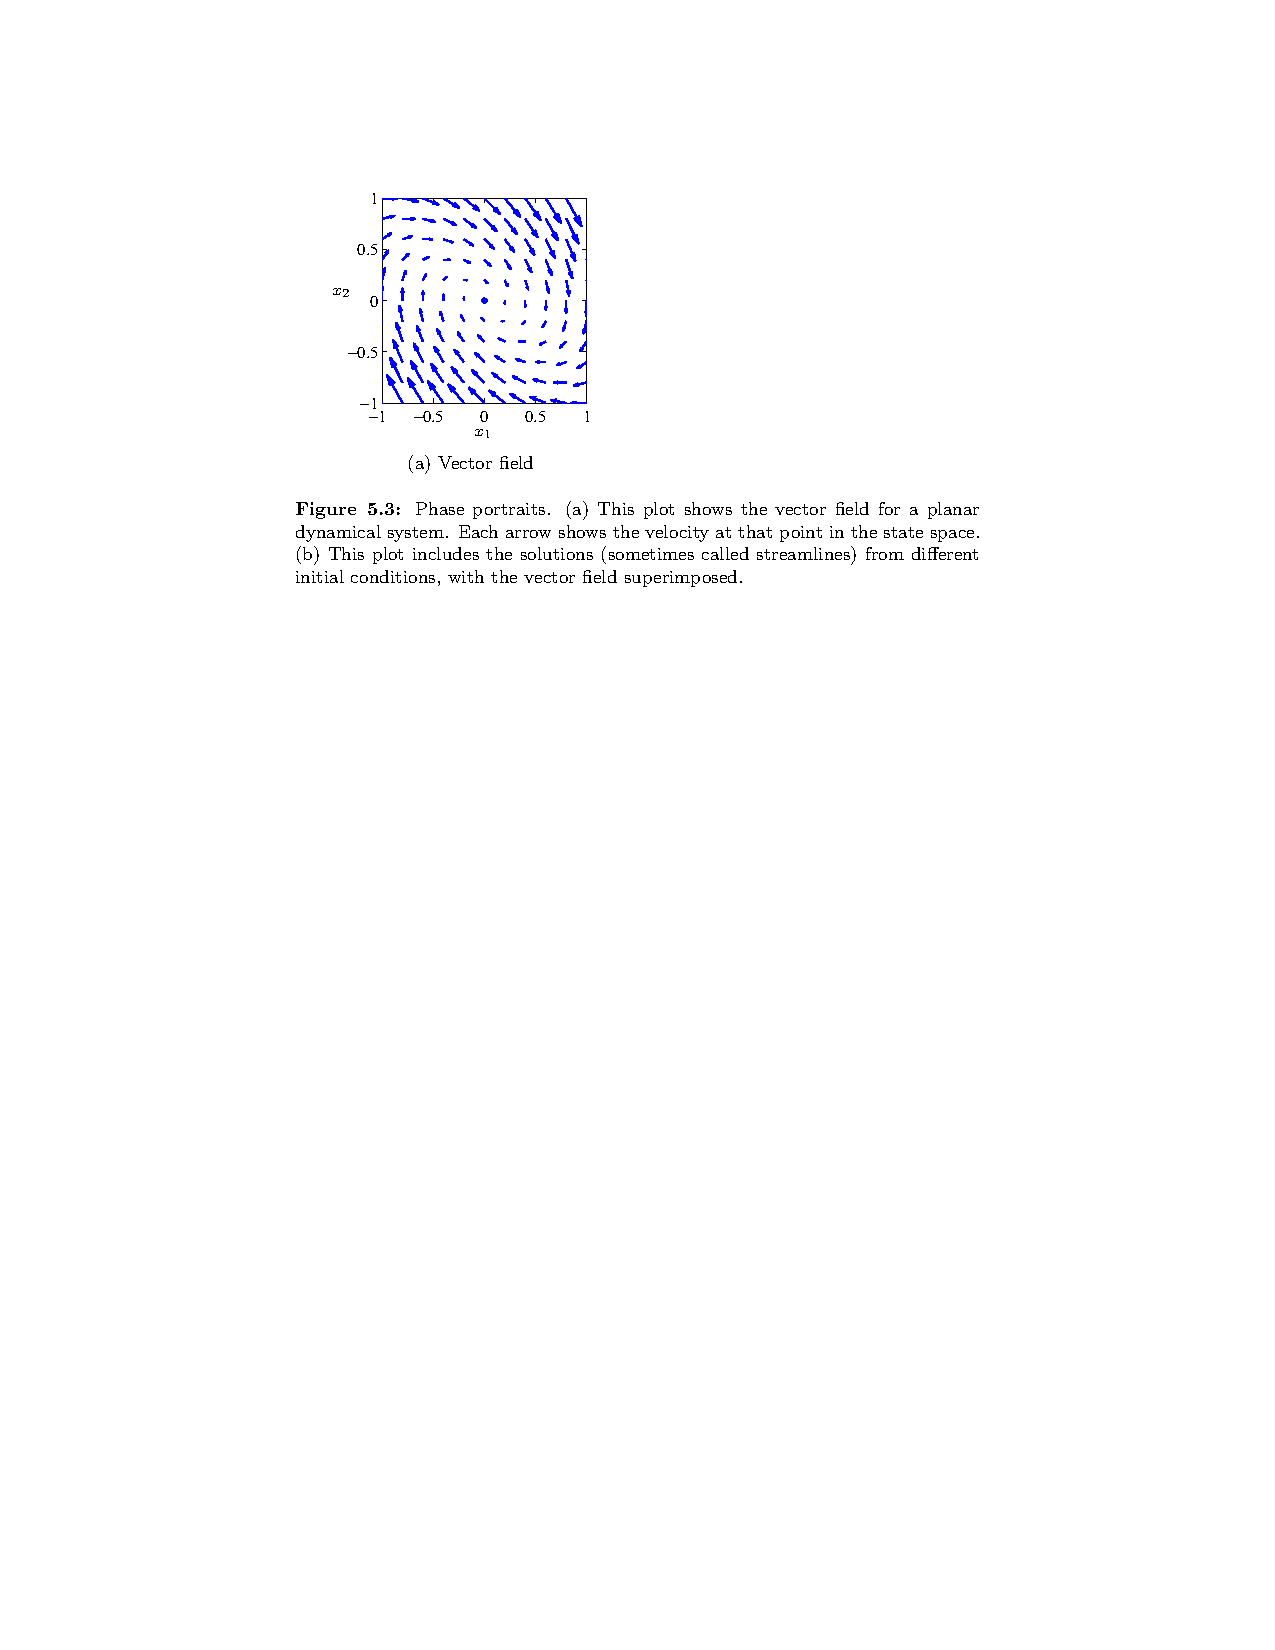
\includegraphics[width=\linewidth]{figure5.3a}
\end{frame}

\begin{frame}
\frametitle{Phase portrait}
\begin{itemize}
\item The vector field is best at highlighting stationary points
\item You can infer but can't directly visualise trajectories
\item Enter the `phase portrait' --- a superimposed collection of trajectories 
\item Where the trajectories cluster and converge tells us important properties of the system
\item Note that trajectories don't tell us rate of change
\end{itemize}
\end{frame}

\begin{frame}
\frametitle{Phase portrait plot}
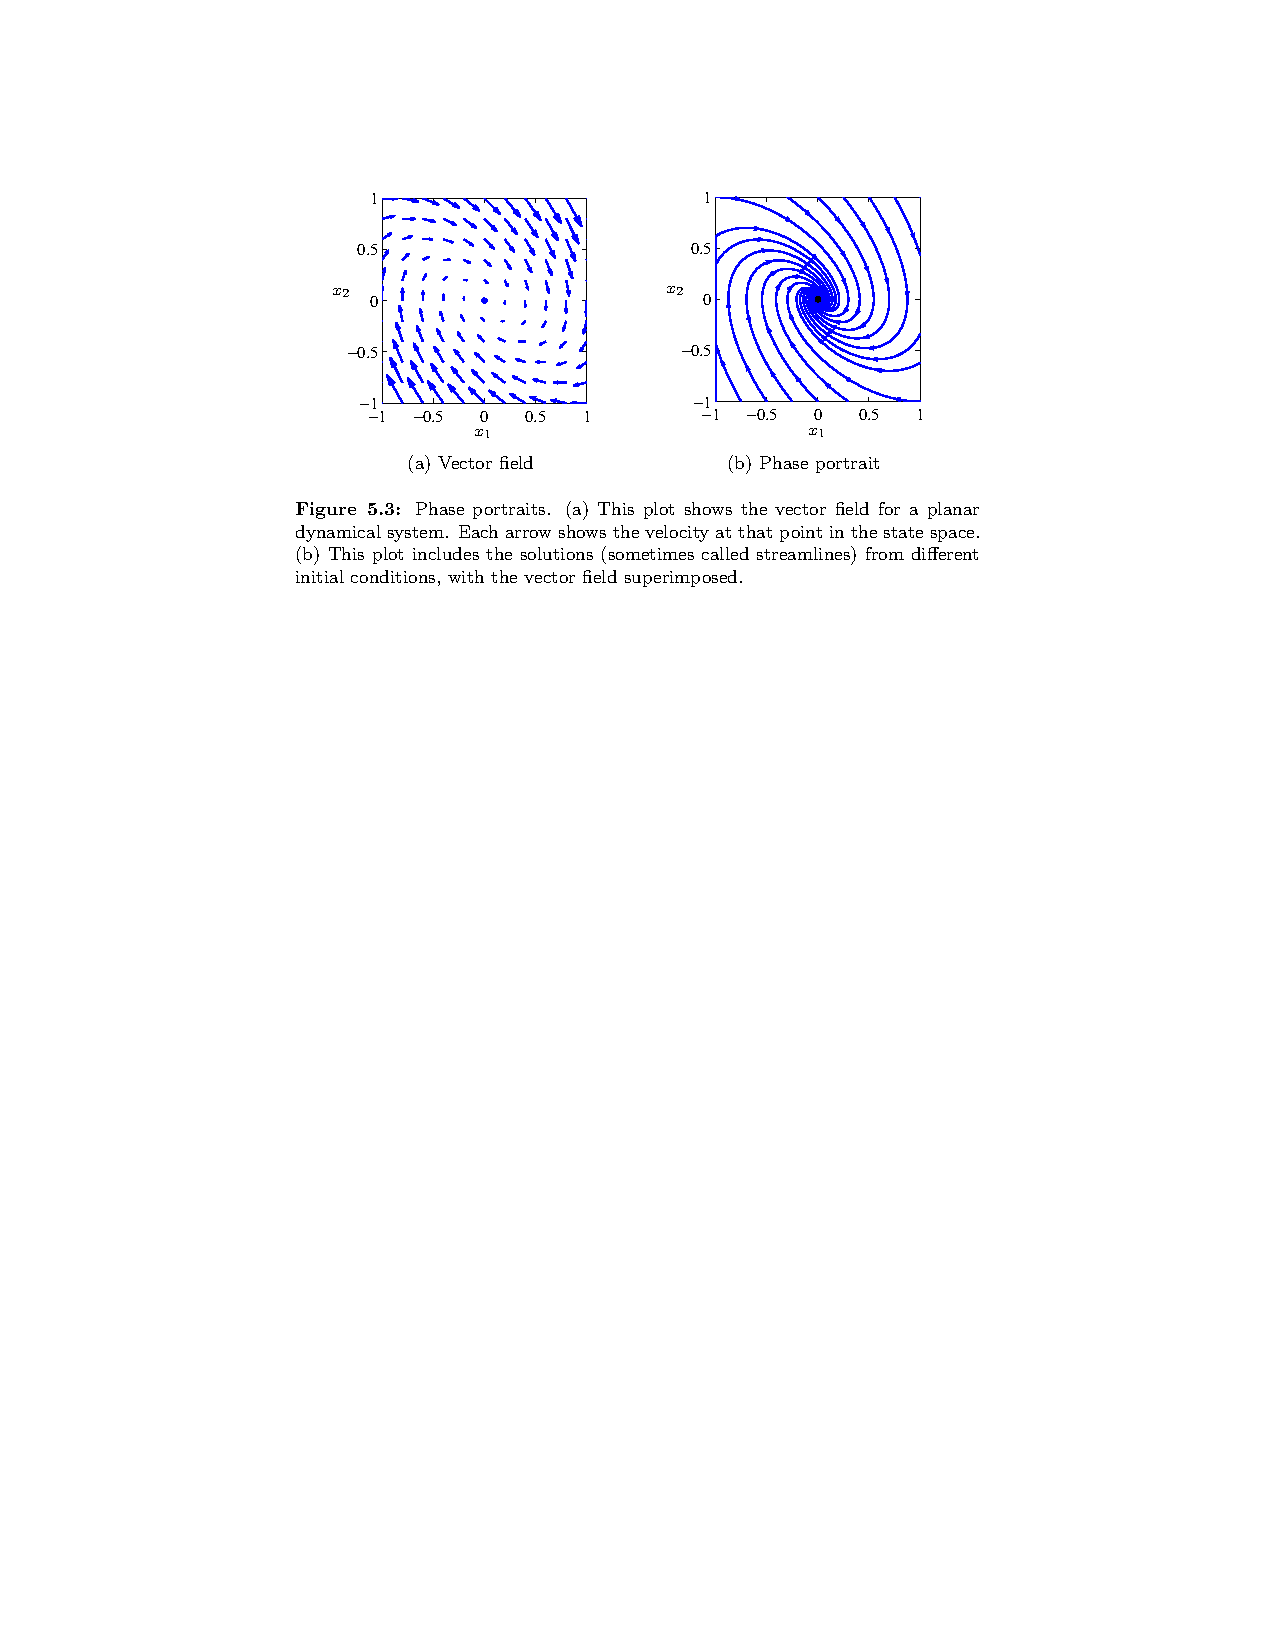
\includegraphics[width=\linewidth]{figure5.3b}

\end{frame}

\SUBCONCEPT{Equilibrium Points and Limit Cycles}

\begin{frame}{This is another slide}
\begin{itemize}
\item c
\item d
\end{itemize}
\end{frame}


\SUMMARYFRAME
\FINALE

\end{document}

  \documentclass{beamer-control}
\usepackage{beamer-control-singlefile}
\INCLUDEONLY{Stability}
\begin{document}
\CONCEPT{Stability}

\begin{SUMMARY}
\begin{itemize}
\item Yyy
\end{itemize}
\vfill References:
\begin{itemize}
\item \astrom{Chapter Z}
\end{itemize}
\end{SUMMARY}



\SUBCONCEPT{This is a Subconcept}

\begin{frame}{This is a slide}
\begin{itemize}
\item a
\item b
\end{itemize}
\end{frame}


\SUBCONCEPT{This is another Subconcept}

\begin{frame}{This is another slide}
\begin{itemize}
\item c
\item d
\end{itemize}
\end{frame}


\SUMMARYFRAME
\FINALE

\end{document}

  \documentclass{beamer-control}
\usepackage{beamer-control-singlefile}
\INCLUDEONLY{Examples}
\begin{document}
\CONCEPT{Examples}

\begin{SUMMARY}
\begin{itemize}
\item Yyy
\end{itemize}
\vfill References:
\begin{itemize}
\item \astrom{Chapter Z}
\end{itemize}
\end{SUMMARY}



\SUBCONCEPT{This is a Subconcept}

\begin{frame}{This is a slide}
\begin{itemize}
\item a
\item b
\end{itemize}
\end{frame}


\SUBCONCEPT{This is another Subconcept}

\begin{frame}{This is another slide}
\begin{itemize}
\item c
\item d
\end{itemize}
\end{frame}


\SUMMARYFRAME
\FINALE

\end{document}


\TOPIC{Linear Systems}

  \documentclass{beamer-control}
\usepackage{beamer-control-singlefile}
\INCLUDEONLY{Basic Definitions}
\begin{document}
\CONCEPT{Basic Definitions}

\begin{SUMMARY}
\begin{itemize}
\item Linearity
\item Time invariance
\end{itemize}
\vfill References:
\begin{itemize}
\item \astrom{§6.1}
\end{itemize}
\end{SUMMARY}



\SUBCONCEPT{Linearity}

\begin{frame}
\frametitle{Static gain models}
\begin{itemize}
\item Vary input $r=10\%\dots100\%$ (say)
\item Record steady state output vs control input
\item For linear models, slope will be constant
\item For nonlinear models, non-constant slope
\item E.g., rubber or magnetic spring
\end{itemize}
\end{frame}


\begin{frame}[fragile]

\newcommand{\myfig}[6]{%
\begin{scope}[xshift=#6,
             spring/.style = {decorate,
                              decoration = {aspect         = 0.5,
                                            segment length = #1,
                                            amplitude      = 2mm,
                                            coil}}]

\path (0,0)                            coordinate (g)
      (0,-0.5cm)                       coordinate (topspring)
      (0,#2)                           coordinate (bottomspring)
      (bottomspring) ++(0,-.5cm)       coordinate (pt2)
                      +(0cm,-#3)       coordinate (pt3)
                      +(1.25cm,-#3)    coordinate (#5 pt3);

 \node [platform,
        anchor = south] at (g)  {};
 \draw [very thick]    (-1,0)         -- (1,0);
 \draw                (topspring)     -- (g)
                      (bottomspring)  -- (pt2.north);
 \draw [spring]       (bottomspring)  -- (topspring);
 \draw [] (pt3) circle (#3)
                          node[inner sep = 0,
                               scale     = #4,
                               text      = black]{$m_{#5}$};
% \node[right=1.5*#3] at (pt3) {#5} ;
 \end{scope}
}

\begin{tikzpicture}[thick,
                    every node/.style = {draw      = none,
                                         inner sep = 0pt,
                                         outer sep = 0pt},
                    platform/.style   = {fill,
                                         pattern = north east lines,
                                         minimum width  = 2cm,
                                         minimum height  =0.3cm}]
 \myfig{1mm}{-2cm}{0.20cm}{0.5}{A}{-2cm}
 \myfig{3mm}{-3cm}{0.28cm}{0.8}{B}{ 0cm}
 \myfig{3mm}{-4cm}{0.39cm}{1.1}{C}{ 2cm}

\draw[dashed]  (A pt3)  +(-0.4,0)     --               +(0.4,0)
                        +(-0.4+2,0) -- coordinate (b1) +(0.4+2,0)
               (B pt3)  +(-0.4-2,0) -- coordinate (a2) +(0.4-2,0)
               (C pt3)  +(-0.4-2,0) -- coordinate (b2) +(0.4-2,0) ;

\draw[latex-latex] (A pt3) -- node[right=0.1cm]{} (a2);
\draw[latex-latex] (b1)    -- node[right=0.1cm]{} (b2);

\end{tikzpicture}

\end{frame}


\begin{frame}
\frametitle{Linear vs Affine}

\begin{align}
m\ddot x &= -c\dot x - k (x-l_0) - mg + f
\end{align}
\begin{itemize}
\item What is the spring force for $x = l_0$ ?
\item What is the spring force at equilibrium $x_e$ ?
\item Note that 
\end{itemize}
\begin{align}
\Deriv{(x-l_0)}{t} =
\Deriv{(x-x_e)}{t} =
\Deriv{(x)}{t}
\end{align}
So:
\begin{align}
m\ddot {\tilde{x}} &= -c\dot{\tilde x} - k \tilde{x} + f
\end{align}

\end{frame}

\begin{frame}
\frametitle{Affine state space}
Translating systems to their equilibrium point is often \emph{required} due to the form of the state space equations:
\begin{align}
\Deriv{x}{t} = \Matr{\dot x\\\ddot x} = Ax + Bu = \Matr{0 & 1\\ -\frac km & -\frac cm } \Matr{x \\ \dot x} + Bu
\end{align}
Note that there is no constant term!\footnote{Let's just say we \emph{could} include it through  $Bu$  but it's not a good idea.}
\end{frame}

\begin{frame}
\frametitle{Linearity of solutions}
\begin{itemize}
\item<uncover@1-> Principle of superposition:
\begin{itemize}
\item Solution from scaled input $y(\alpha x_0)=\alpha y(x_0)$
\item Solution from multiple inputs $y(x_1+x_2)=y(x_1)+y(x_2)$
\item Etc.\ for $u$
\end{itemize}
\item<uncover@2-> Therefore we often consider:
\begin{itemize}
\item Solution to the homogeneous (or unforced) system \[\Deriv{x_h}{t}=Ax_h\]
\item Solution to the particular (or forced) system \[\Deriv{x_p}{t}=Ax_p+Bu\]
\item And their combinations --- see textbook Example 6.1
\end{itemize}
\end{itemize}
\end{frame}


\SUBCONCEPT{Time invariance}

\begin{frame}{Timey wimey}
Time invariance is a subtle concept:
\begin{itemize}
\item Of course solutions to $\Deriv{x}{t} = Ax$ are time-dependent
\item What we mean is $y_2(t+a) = y_1 (t)$ if $u_2(t+a) = u_1 (t)$
\end{itemize}
\end{frame}

\begin{frame}
\frametitle{Superposition across time}

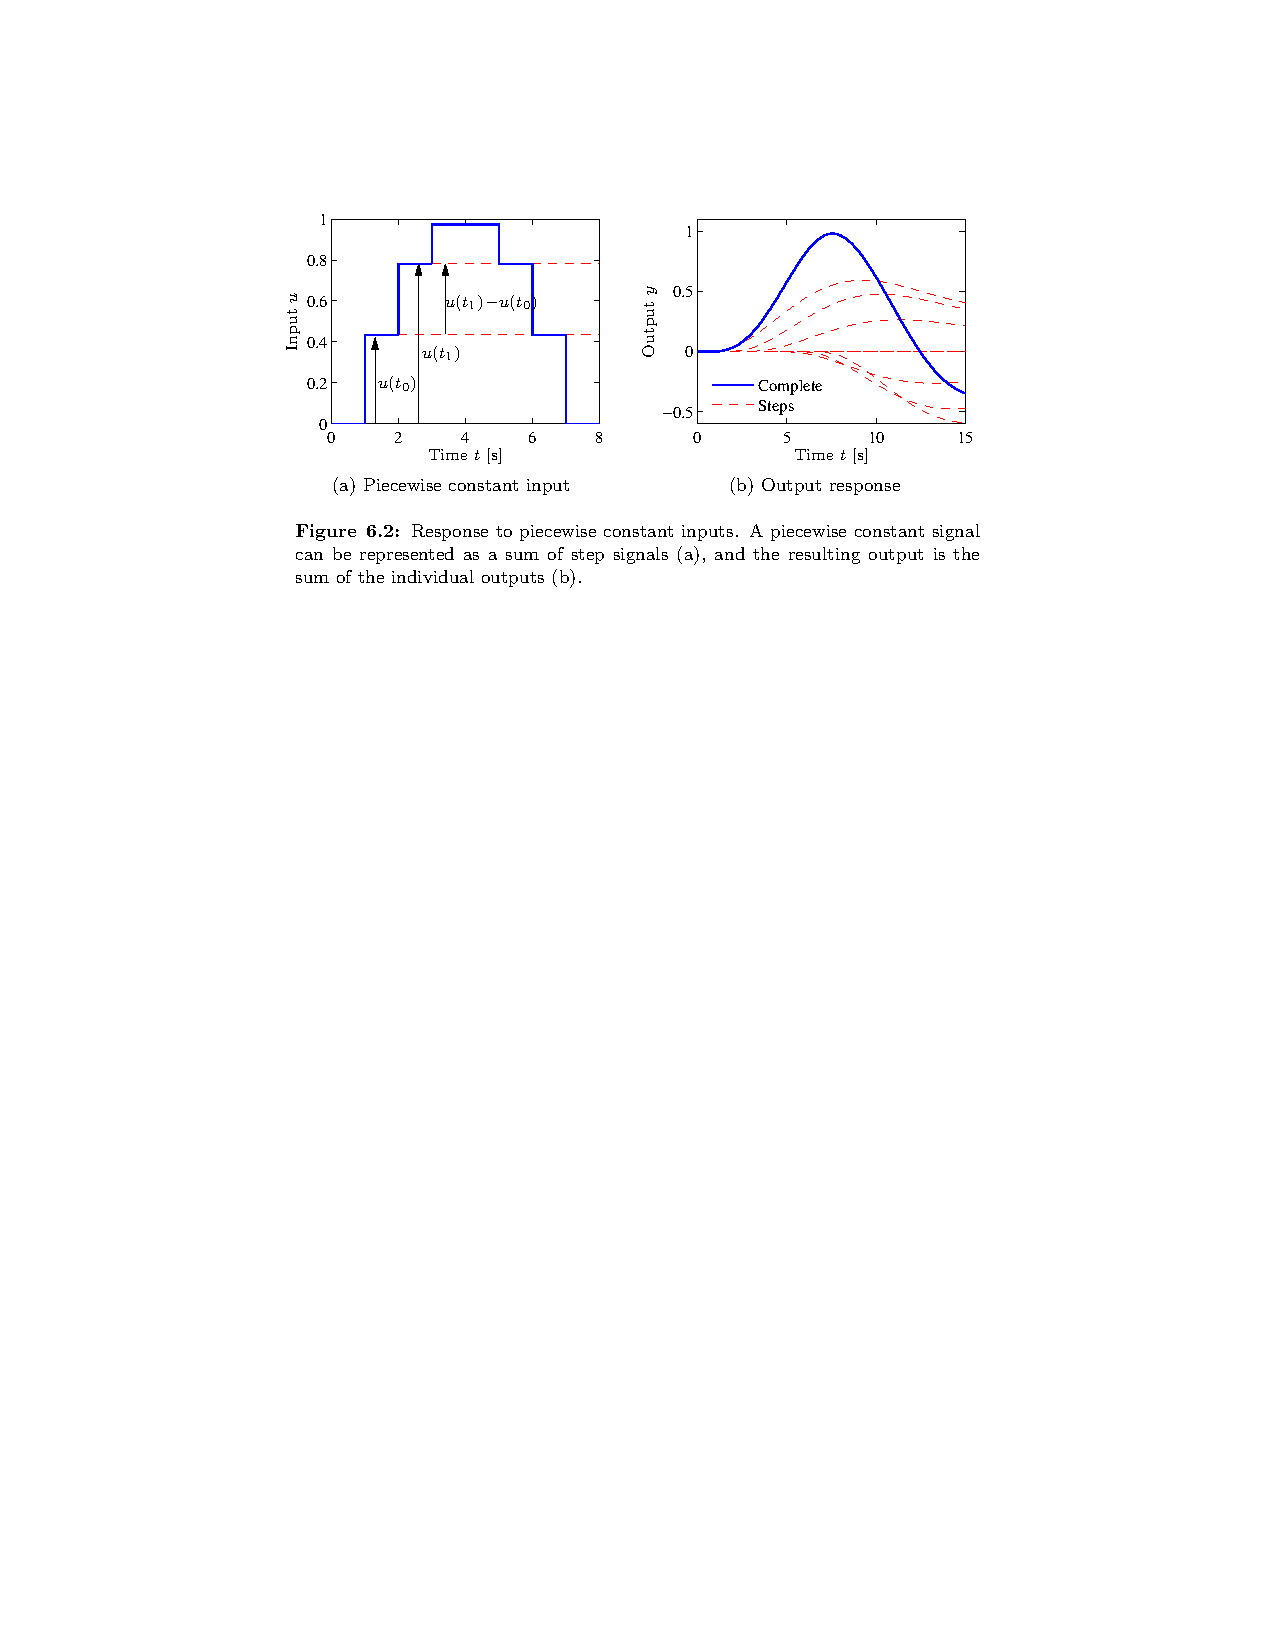
\includegraphics[width=\linewidth]{figure6.2}


\end{frame}

\begin{frame}
\frametitle{LTI systems}
\begin{itemize}
\item When is a system not time invariant? Consider, e.g.:
\begin{itemize}
\item a rubber with stiffness that changes with temperature
\item non-Newtonian material with velocity-dependent damping
\item a rocket with fuel mass that burns away over time
\end{itemize}
\item All of classical control theory assumes we have linear, time-invariant (LTI) systems
\item These are generally \emph{good approximations} for most engineering systems
\item Errors due to these assumptions are often handled gracefully by the control system
\item Adaptive and/or nonlinear control is needed for more complex systems
\end{itemize}
\end{frame}

\SUMMARYFRAME
\FINALE

\end{document}

  \documentclass{beamer-control}
\usepackage{beamer-control-singlefile}
\INCLUDEONLY{The Matrix Exponential}
\begin{document}
\CONCEPT{The Matrix Exponential}

\begin{SUMMARY}
\begin{itemize}
\item Initial Condition Response
\item Diagonal and Jordan forms
\end{itemize}
\vfill References:
\begin{itemize}
\item \astrom{§6.2}
\end{itemize}
\end{SUMMARY}



\SUBCONCEPT{Initial Condition Response}

\begin{frame}{Generalising system output}
We have shown:
\begin{align}\label{eq:impresp}
y(t) = \int^t_0 \ImpulseResponse(t-\tau)u(\tau)\dee\tau
\end{align}
This form assumes zero initial conditions.

In this concept we:
\begin{itemize}
\item generalise  \eqref{impresp},
\item particularly for nonzero initial conditions.
\end{itemize}
\end{frame}

\begin{frame}
\frametitle{Consider $u=0$}
For unforced system:
\begin{align}
\dot x = A x
\end{align}
For scalar $A=a$, the solution is (naturally)
\begin{align}
x(t) = \ee^{at}x(0)
\end{align}
But note that $a$ could be complex!
\end{frame}

\begin{frame}
\frametitle{For multiple states}

For matrix $A$, we define solution
\begin{align}
x(t) = \ee^{At} x(0)
\end{align}
where $\ee^{At}$ is the \alert{matrix exponential}.
\bigskip

\begin{uncoverenv}<2>
Define $\ee^{At}$ using Taylor series:
\begin{align}
\ee^{At} = I + At + \tfrac12 A^2t^2 + \tfrac{1}{3!}A^3+t^3 + \cdots = \sum_{k=0}^{\infty} \tfrac{1}{k!}A^kt^k
\end{align}
As expected: $\Deriv{}{t} \ee^{At} = A \ee^{At}$
\end{uncoverenv}
\end{frame}

\begin{frame}
\frametitle{Linearity of solutions}
Example two-state system:
\begin{align}
x(t) = \Matr{x_1\\x_2} = \ee^{At}\Matr{x_1(0)\\x_2(0)}
\end{align}
\begin{uncoverenv}<2->
Find solutions:
\begin{align}
x_{h1}(t) &= \ee^{At}\Matr{x_{1,0}\\0} &
x_{h2}(t) &= \ee^{At}\Matr{0\\x_{2,0}} 
\end{align}
\end{uncoverenv}
\begin{uncoverenv}<3->
For arbitrary initial condition:
\begin{align}
\ee^{At}\Matr{\alpha x_{1,0}\\\beta x_{2,0}} = \ee^{At}\Matr{\alpha x_{1,0}\\0} + \ee^{At}\Matr{0\\\beta x_{2,0}} = \alpha x_{h1}(t) + \beta x_{h2}(t)
\end{align}
\end{uncoverenv}
\end{frame}

\begin{frame}
\frametitle{Oscillator examples}
For undamped oscillator (mass-spring):
\begin{align}
\ddot q + \ww_0^2 q  = u
\end{align}
Dynamics are normalised using $x_1=q$, $x_2 = \dot q/\ww_0$:
\begin{align}
A &= \Matr{0 & \ww_0\\ -\ww_0 & 0} & \ee^{At} &= \Matr{ \cos \ww_0 t & \sin \ww_0 t \\ -\sin \ww_0 t & \cos \ww_0 t}
\end{align}
Therefore:
\begin{align}
x(t) = \ee^{At} x(0) = \Matr{ \cos \ww_0 t & \sin \ww_0 t \\ -\sin \ww_0 t & \cos \ww_0 t} \Matr{x_1(0)\\ x_2(0)}
\end{align}
\end{frame}

\begin{frame}
\frametitle{Oscillator examples}
For damped oscillator (mass-spring-damper):
\begin{align}
\ddot q + 2 \zz \ww_0 \dot q + \ww_0^2 q  = u
\end{align}
Skipping to the solution:
\begin{align}
x(t) = \ee^{At} x(0) = \ee^{-\zz\ww_0 t} \Matr{ \cos \ww_d t & \sin \ww_d t \\ -\sin \ww_d t & \cos \ww_d t} \Matr{x_1(0)\\ x_2(0)}
\end{align}
where $\wdamp = \ww_0 \sqrt{1-\zz^2}$ (damped natural frequency)
\end{frame}



\SUBCONCEPT{Diagonal and Jorden forms}

\begin{frame}
\frametitle{Diagonal forms}
In the undamped example, $A = \left[\begin{smallmatrix} 0 & \ww_0\\ -\ww_0 & 0\end{smallmatrix}\right]$ and we saw the solution was a linear combination of components.

\bigskip
For larger matrices, can generalise to \alert{diagonal form}:\footnote{\alert{This is the standard convention, opposite the textbook!}}
\begin{align}
\Deriv{x}{t} &= Ax & x &= Tz & \Deriv{z}{t} &= T^{-1}ATz = Jz
\end{align}
(Transformed states $z$ are non-physical)

\end{frame}

\begin{frame}[fragile]
\frametitle{Diagonal $A$ matrix}
Find in Matlab with:
\begin{lstlisting}[style=Matlab-editor]
[T,J] = jordan(A)
\end{lstlisting}
For $A = \left[\begin{smallmatrix} 0 & \ww_0\\ -\ww_0 & 0\end{smallmatrix}\right]$:
\begin{align}
T &= \Matr{ \ii & -\ii \\ 1 & 1  } & J &= T^{-1}AT = \Matr{ -\ww_0 \ii & 0 \\ 0 & \ww_0 \ii}
\end{align}
We can now see intuitively that the solutions will be of the form $\ee^{\ii \ww_0 t}$ which are sinusoids.
\end{frame}

\begin{frame}
\frametitle{Generalised diagonal matrix}
Recall solutions are in the form
\begin{align}
\ee^{At} = I + At + \tfrac12 A^2t^2 + \tfrac{1}{3!}A^3+t^3 + \cdots = \sum_{k=0}^{\infty} \tfrac{1}{k!}A^kt^k
\end{align}
For diagonal $A$ matrices:
\begin{align}
A &= \Matr{ \lambda_1 &  &  & 0 \\  & \lambda_2 &  &  \\  &  & \ddots &  \\ 0 &  &  & \lambda_n } \,, &
(At)^k &= \Matr{ \lambda_1^kt^k &  &  & 0 \\  & \lambda_2^kt^k &  &  \\  &  & \ddots &  \\ 0 &  &  & \lambda_n^kt^k }
\end{align}
Combining:
\begin{align}\label{eq:diagform}
\ee^{At} = \Matr{ \ee^{\lambda_1 t} &  &  & 0 \\  & \ee^{\lambda_2 t} &  &  \\  &  & \ddots &  \\ 0 &  &  & \ee^{\lambda_n t} }
\end{align}

\end{frame}

\begin{frame}
\frametitle{Jordan form}
\begin{itemize}
\item Diagonal transformations can't get us to \eqref{diagform} if we have repeated eigenvalues ($\lambda_i=\lambda_j$)
\item In this case couple $k$ number of systems together:
\end{itemize}
\begin{align}
J   &= \Matr{ J_1 &  &  & 0 \\  & J_2 &  &  \\  &  & \ddots &  \\ 0 &  &  & J_k } \,, &
J_i &= \Matr{ \lambda_{i,1} & 1 &  & 0 \\  & \lambda_{i,2} & 1 &  \\  &  & \ddots &  \ddots \\ 0 &  &  & \lambda_{i,j} }
\end{align}
\end{frame}

\begin{frame}
\frametitle{Jordan form solution}
\begin{itemize}
\item Any square matrix can be written in Jordan form \AMref{Theorem 6.2}
\item Once in Jordan form, solution comes as:
\end{itemize}
\begin{align}
\ee^{At} = \Matr{ \ee^{J_1 t} &  &  & 0 \\  & \ee^{J_2 t} &  &  \\  &  & \ddots &  \\ 0 &  &  & \ee^{J_k t} }
\end{align}
with $\ee^{J_i t}$ given along subsequent lines \AMref{Eq (6.11)}
\end{frame}

\begin{frame}
\frametitle{The big reveal}
\begin{itemize}
\item All of this maths is to bring is to a fundamental truth which links linear algebra to ordinary differential equations
\item How do we look at an $A$ matrix to determine the properties of the system?
\item Transformations of $A$ bring us to Jordan form, where see all solutions in terms of $\lambda_i$ eigenvalues:
\end{itemize}
\begin{align}
\ee^{\lambda t} = \ee^{(\sigma + \ii \ww)t} = \ee^{\sigma t} ( \cos \ww t + \ii \sin \tt t)
\end{align}
Stability comes from $\sigma$, therefore:
\begin{theorem}
The system $\dot x=Ax$ is asymptotically stable if and only if all eigenvalues of $A$ have a strictly negative
real part and is unstable if any eigenvalue of $A$ has a strictly positive real part.
\end{theorem}
\end{frame}



\SUMMARYFRAME
\FINALE

\end{document}

  \documentclass{beamer-control}
\usepackage{beamer-control-singlefile}
\INCLUDEONLY{Input/Output Response}
\begin{document}
\CONCEPT{Input/Output Response}

\begin{SUMMARY}
\begin{itemize}
\item Yyy
\end{itemize}
\vfill References:
\begin{itemize}
\item \astrom{Chapter Z}
\end{itemize}
\end{SUMMARY}



\SUBCONCEPT{This is a Subconcept}

\begin{frame}{This is a slide}
\begin{itemize}
\item a
\item b
\end{itemize}
\end{frame}


\SUBCONCEPT{This is another Subconcept}

\begin{frame}{This is another slide}
\begin{itemize}
\item c
\item d
\end{itemize}
\end{frame}


\SUMMARYFRAME
\FINALE

\end{document}

  \documentclass{beamer-control}
\usepackage{beamer-control-singlefile}
\INCLUDEONLY{Linearisation}
\begin{document}
\CONCEPT{Linearisation}

\begin{SUMMARY}
\begin{itemize}
\item Jacobian Linearisation
\item Feedback Linearisation
\end{itemize}
\vfill References:
\begin{itemize}
\item \astrom{§6.4}
\end{itemize}
\end{SUMMARY}



\SUBCONCEPT{Jacobian Linearisation}

\begin{frame}{Linearisation steps}
We have nonlinear systems but can often model them linearly:
\begin{itemize}
\item Find or define equilibrium point
\item Shift coordinates so $x_e=0$
\item Make small angle approximations (e.g., $\sin\theta\approx\theta$ for $\theta\approx 0$)
\item More generally, use Taylor series expansion at the equilibrium point and truncate
\end{itemize}
\end{frame}

\begin{frame}
\frametitle{Taylor series expansion}
The Taylor series of differentiable function $f$ about point $a$ is:
\begin{align}
f(x) = f(a) + f'(a)(x - a) + \frac{f''(a)}{2!}(x - a)^2 + \cdots
\end{align}

\begin{align}
x^2 = a^2 + 2a(x - a) + (x - a)^2
\end{align}

\begin{align}
\ee^x = \sum_{n=0}^{\infty} \frac{x^n}{n!} = 1 + x + \frac{x^2}{2!} + \frac{x^3}{3!} + \cdots
\end{align}

\begin{align}
\sin(x) = \sum_{n=0}^{\infty} \frac{(-1)^n}{(2n+1)!} x^{2n+1} = x - \frac{x^3}{3!} + \frac{x^5}{5!} - \cdots
\end{align}
\end{frame}

\begin{frame}
\frametitle{Taylor series linearisation}
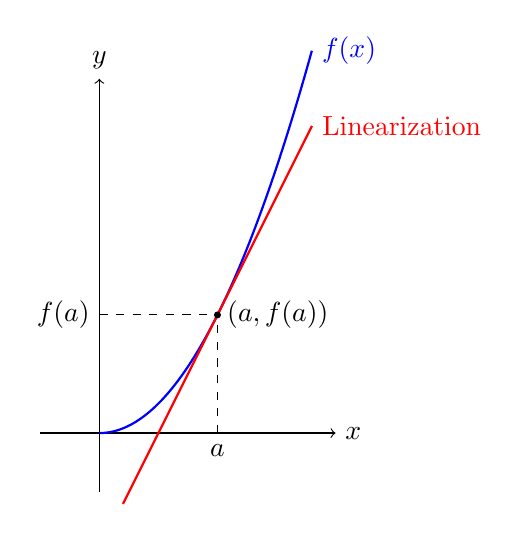
\begin{tikzpicture}[scale=1.5]

  % Axes
  \draw[->] (-0.5,0) -- (2,0) node[right] {$x$};
  \draw[->] (0,-0.5) -- (0,3) node[above] {$y$};

  % Function f(x) = x^2 (example)
  \draw[thick,blue,domain=0:1.8,smooth,samples=100] plot (\x, {\x*\x}) node[right] {$f(x)$};

  % Point a
  \def\a{1}
  \def\fa{\a*\a} % f(a) = a^2
  \def\fpa{2*\a}  % f'(a) = 2a

  % Tangent line at x = a: y = f(a) + f'(a)(x - a)
  \draw[red,thick,domain=0.2:1.8] plot (\x, {\fa + \fpa*(\x - \a)}) node[right] {Linearization};

  % Mark point (a, f(a))
  \filldraw[black] (\a, \fa) circle (0.7pt) node[right] {$(a, f(a))$};

  % Dotted lines to axes
  \draw[dashed] (\a,0) -- (\a,\fa);
  \draw[dashed] (0,\fa) -- (\a,\fa);

  % Labels
  \node at (1, -0.15) {$a$};
  \node[anchor=east] at (0, 1) {$f(a)$};

\end{tikzpicture}

\end{frame}

\begin{frame}
\frametitle{Jacobian linearisation}
The Jacobian $\frac{\partial {f}}{\partial {x}}$ is defined as a matrix of partial derivatives:
\[
{f} : \mathbb{R}^n \to \mathbb{R}^m, \quad
{f}(x_1, x_2, \ldots, x_n) = 
\begin{bmatrix}
f_1(x_1, \ldots, x_n) \\
f_2(x_1, \ldots, x_n) \\
\vdots \\
f_m(x_1, \ldots, x_n)
\end{bmatrix}
\]

\[
\frac{\partial {f}}{\partial {x}} =
\begin{bmatrix}
\frac{\partial f_1}{\partial x_1} & \frac{\partial f_1}{\partial x_2} & \cdots & \frac{\partial f_1}{\partial x_n} \\
\frac{\partial f_2}{\partial x_1} & \frac{\partial f_2}{\partial x_2} & \cdots & \frac{\partial f_2}{\partial x_n} \\
\vdots & \vdots & \ddots & \vdots \\
\frac{\partial f_m}{\partial x_1} & \frac{\partial f_m}{\partial x_2} & \cdots & \frac{\partial f_m}{\partial x_n}
\end{bmatrix}
\]

\end{frame}

\begin{frame}
\frametitle{Jacobian linearisation}
The Jacobian allows a generalised approach. For system:
\begin{align}
\dot x &= f(x,u) & y &= h(x,u)
\end{align}
Define new variables as deviation from equilibrium:
\begin{align}
z &= x - x_e & v &= u - u_e & w&= y-h(x_e,u_e)
\end{align}
Then, linearised system is:
\begin{align}
\dot z &= Az+bv & w &= Cz + Dv
\end{align}
where
\begin{align}
A &= \left.\PDeriv{f}{x}\right|_{(x_e,u_e)} &
B &= \left.\PDeriv{f}{u}\right|_{(x_e,u_e)} &
C &= \left.\PDeriv{h}{x}\right|_{(x_e,u_e)} &
D &= \left.\PDeriv{h}{u}\right|_{(x_e,u_e)}
\end{align}
\end{frame}

\begin{frame}
\frametitle{Example of Jacobian linearisation}
\centering

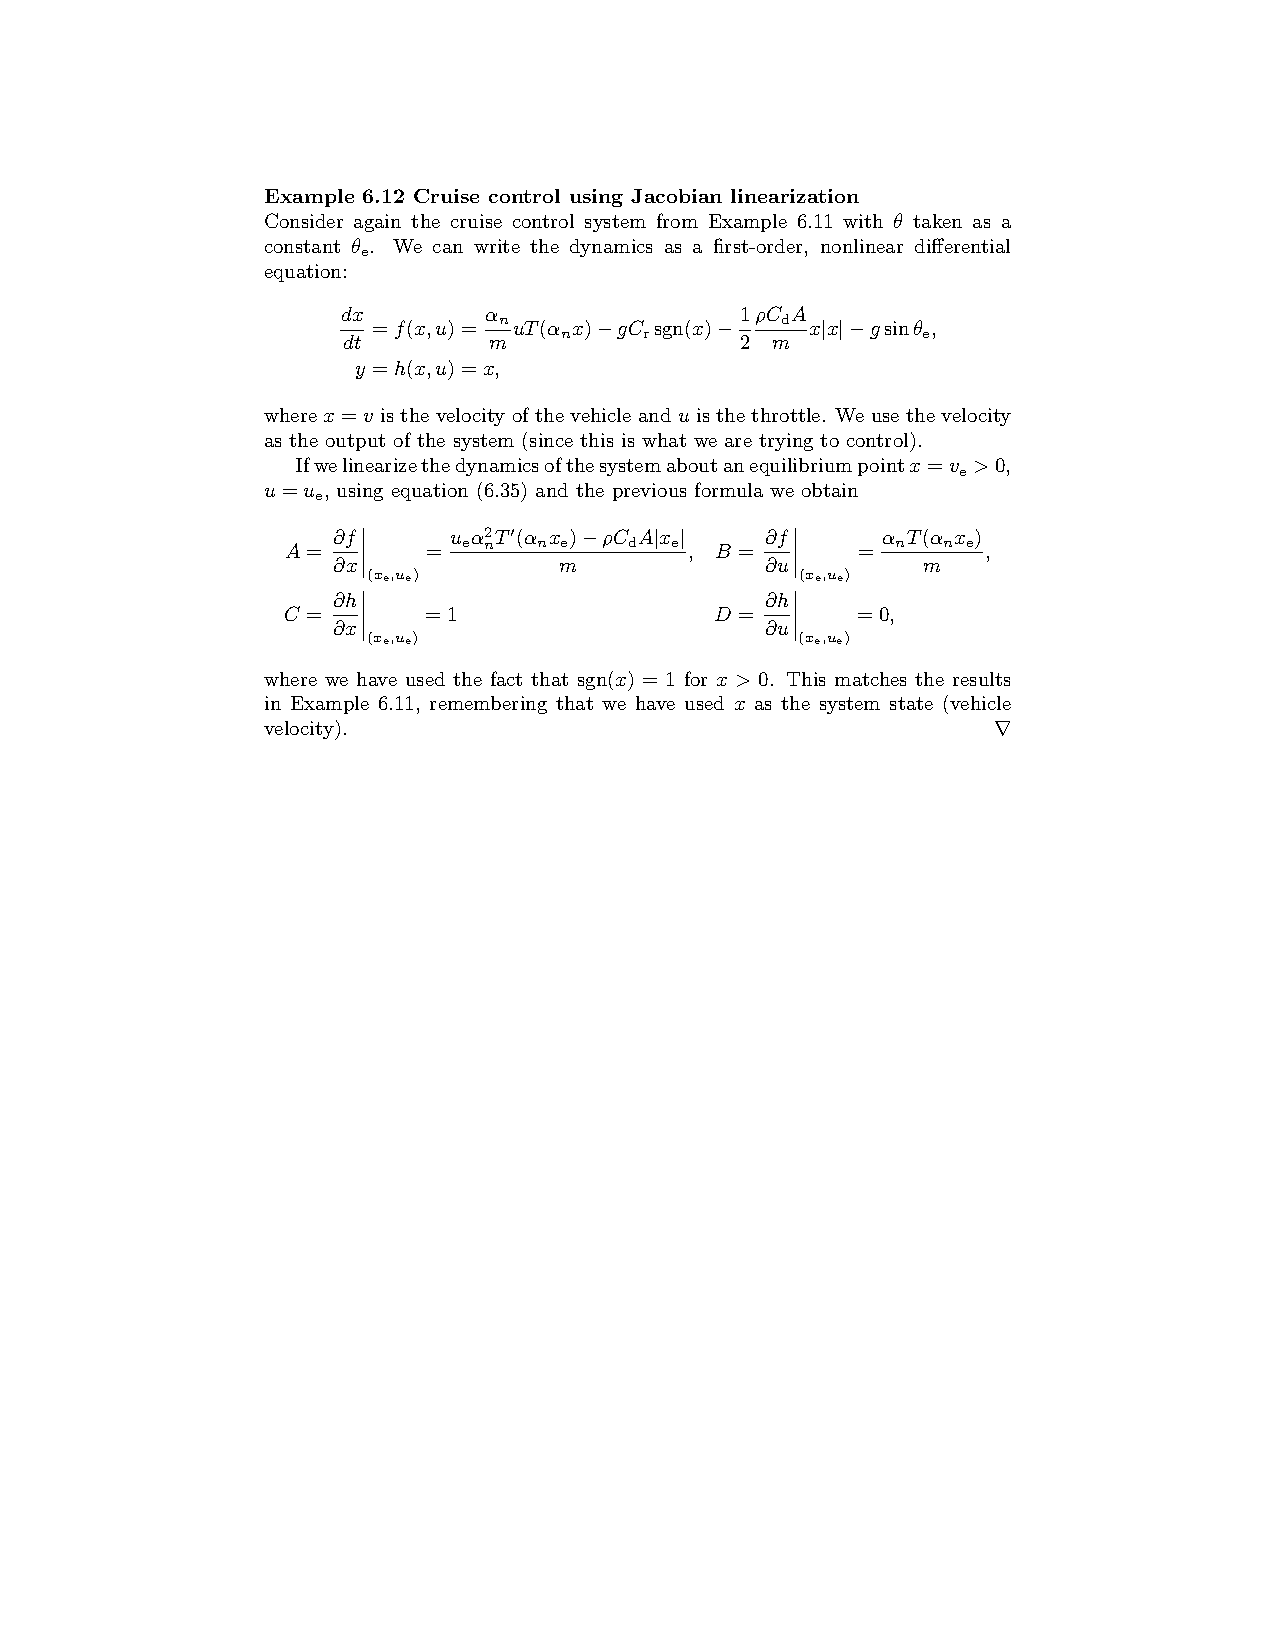
\includegraphics[height=0.8\textheight]{example6.12}

\end{frame}

\SUBCONCEPT{Feedback Linearisation}

\begin{frame}{Feedback Linearisation of quadratic term}
E.g., known nonlinearity $x^2$:
\begin{align}
\dot x &= x^2 + u &
u &= -x^2 - kx
\end{align}
The feedback term `cancels' the nonlinearity and adds a `spring' term
\begin{itemize}
\item
What happens if there is an error between the system $x^2$ term and the controller's?
\end{itemize}
\end{frame}

\begin{frame}
\frametitle{Example of feedback linearisation}
\centering

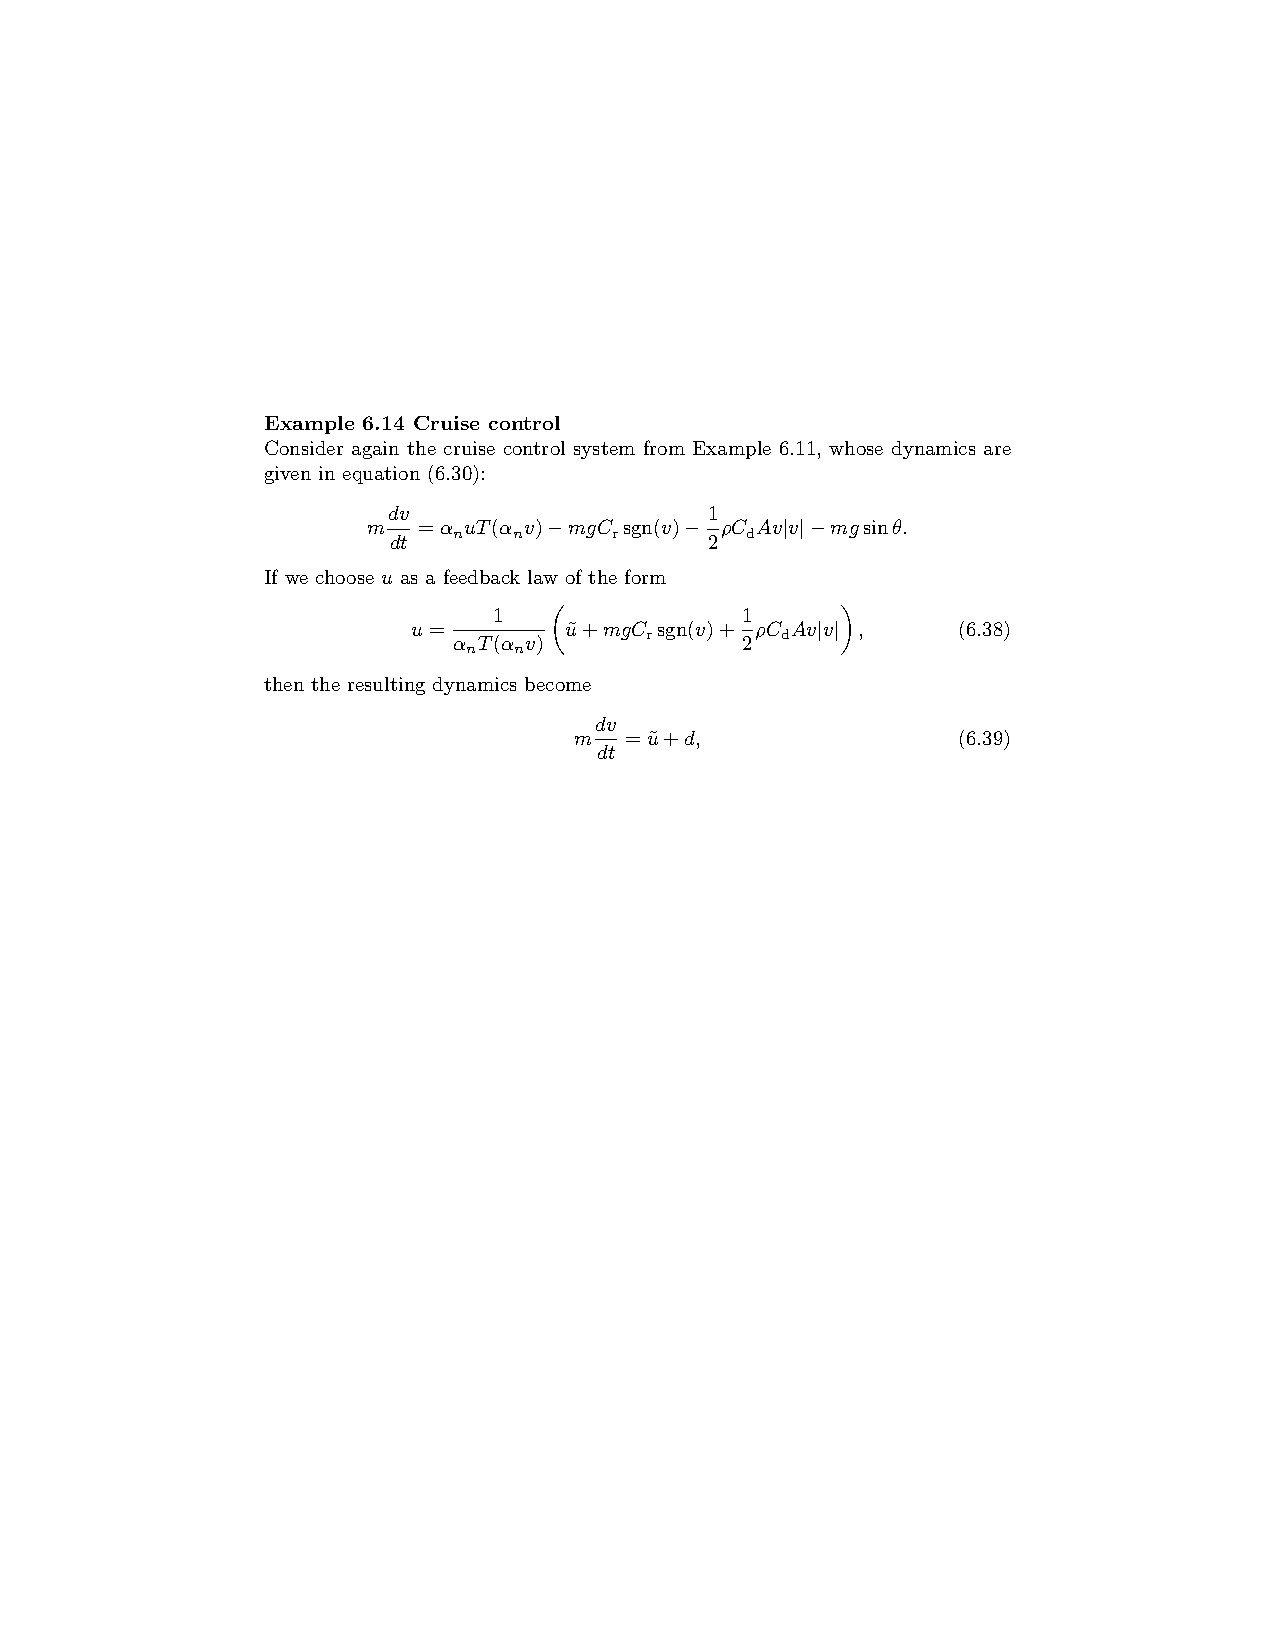
\includegraphics[width=\linewidth]{example6.14}

\end{frame}

\begin{frame}
\frametitle{Block diagram of feedback linearisation}
\centering

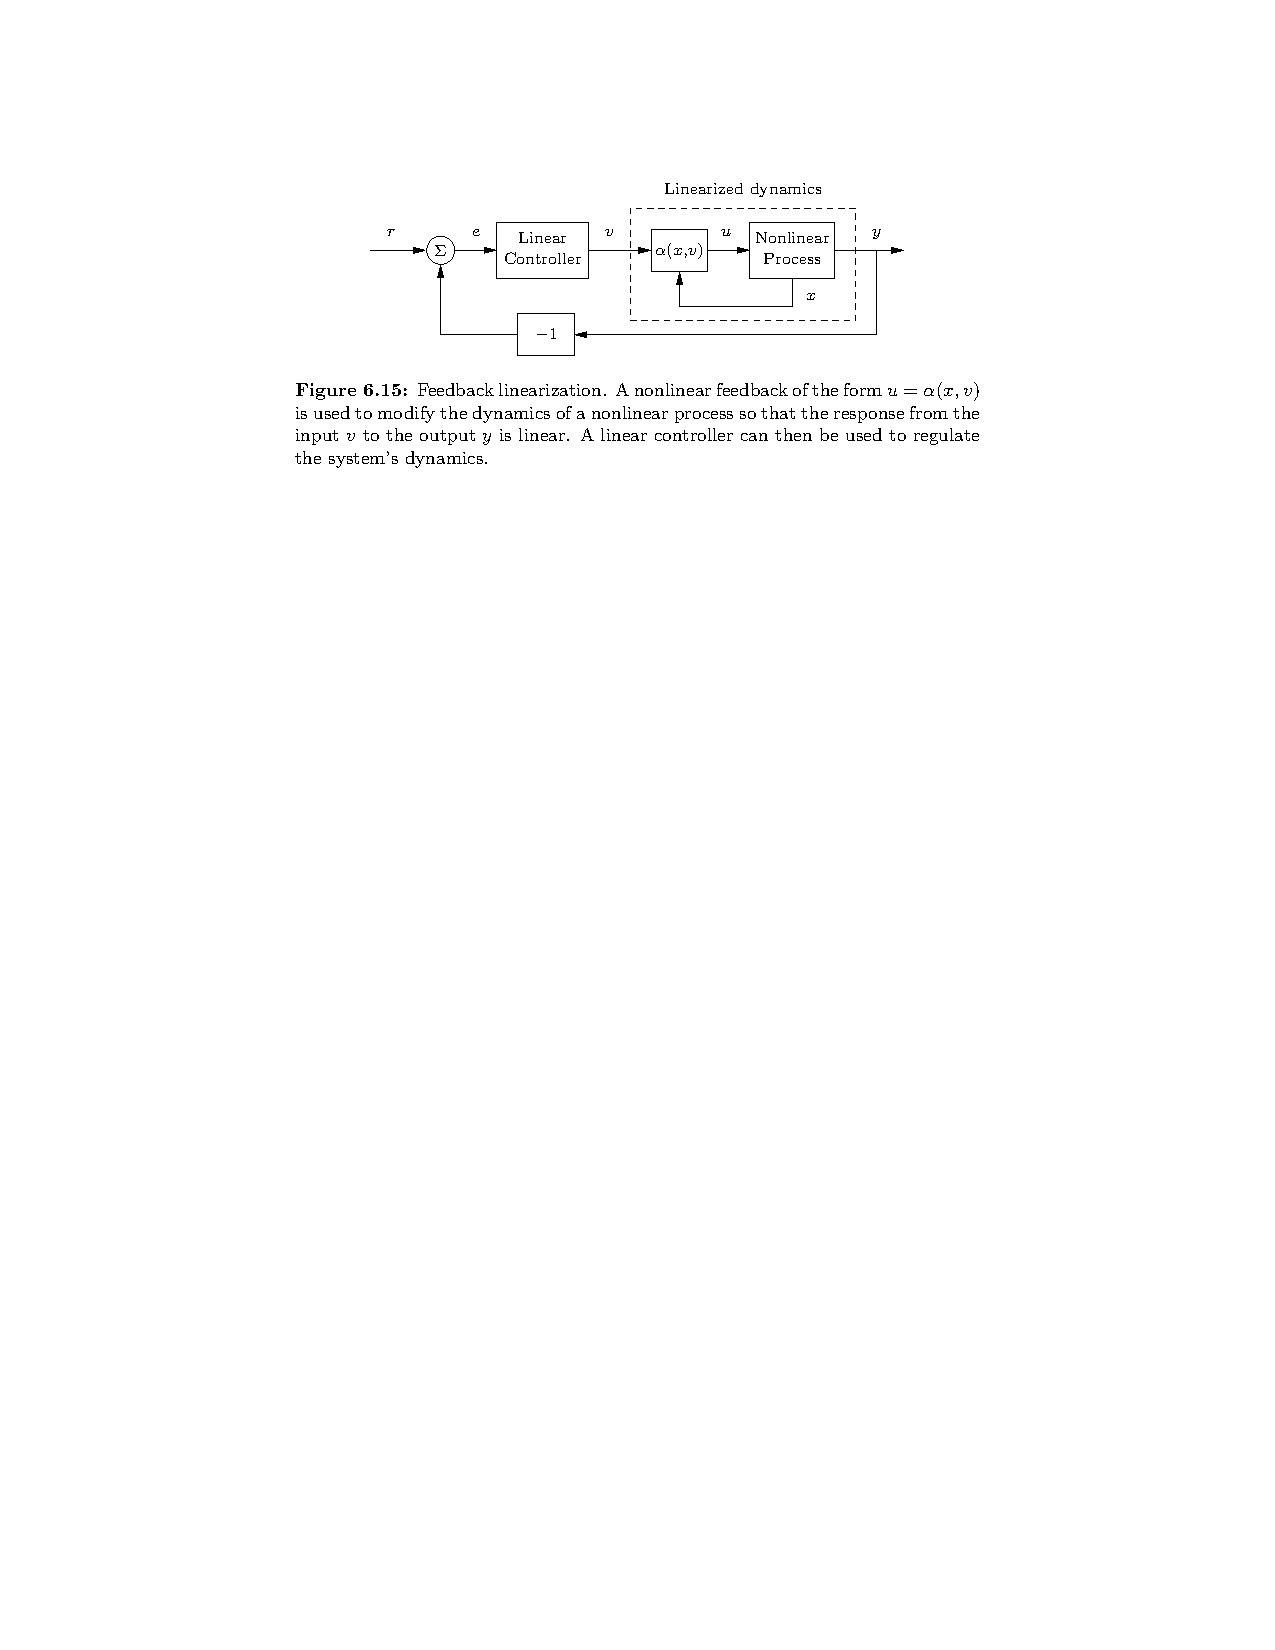
\includegraphics[width=\linewidth]{figure6.15}

\end{frame}

\begin{frame}
\frametitle{Dynamic inversion}
Generalised mechanical system with $M(q)$, $C(q,\dot q)$, $B(q)$:
\begin{align}
M(q)\ddot q + C(q,\dot q) = B(q) u \\
u = B(q)^{-1} \left( M(q) \alert{v} + C(q,\dot q) \right)
\end{align}
Resulting dynamics of the system are:
\begin{align}
M(q)\ddot q &= M(q) \alert{v} & \therefore\qquad \ddot q &= v
\end{align}
All dynamics are cancelled, assuming we can model them accurately and the actuators can react appropriately
\end{frame}

\SUMMARYFRAME
\FINALE

\end{document}



\MODULE{Control System Concepts}


\TOPIC{State Feedback}

  \documentclass{beamer-control}
\usepackage{beamer-control-singlefile}
\INCLUDEONLY{Reachability}
\begin{document}
\CONCEPT{Reachability}

\begin{SUMMARY}
\begin{itemize}
\item Reachability definition
\item Controllability definition
\item Reachability matrix
\item Reachable canonical form
\end{itemize}
\vfill References:
\begin{itemize}
\item \astrom{§7.1}
\end{itemize}
\end{SUMMARY}



\SUBCONCEPT{Definitions}

\begin{frame}{Reachability}
Consider a system where the state evolution is given by the linear state space equations
\[\frac{\mathrm{d} x}{\mathrm{d} t} = Ax+Bu\]
where $x$ is n-dimensional
\begin{itemize}
\item An important question is, is it possible to find a control signal $u(t)$ such that we can reach any state $x$ in the state space given an initial state $x_0$
\item The set of states that can be reached by steering the system with control input $u(t)$ for $0\leq t\leq T$ from an initial state $x_0$ is known as the \textit{reachable set}, $\mathcal{R}(x_0,\leq T)$
\end{itemize}
\end{frame}


\begin{frame}{Reachability}
\begin{itemize}
	\item A linear system is \textit{reachable} if,for any initial state $x_0$ and final state $x_f$, there exists a $T>0$ and control $u(t)$ such that $x(0)=x_0$ and $x(T)=x_f$
	\item In other words, the reachable set $\mathcal{R}(x_0,\leq T)$ is our whole state space
	\item This is essentially saying, we can get anywhere in our state space in finite time, no matter where we start!
\end{itemize}

\begin{figure}
	\centering
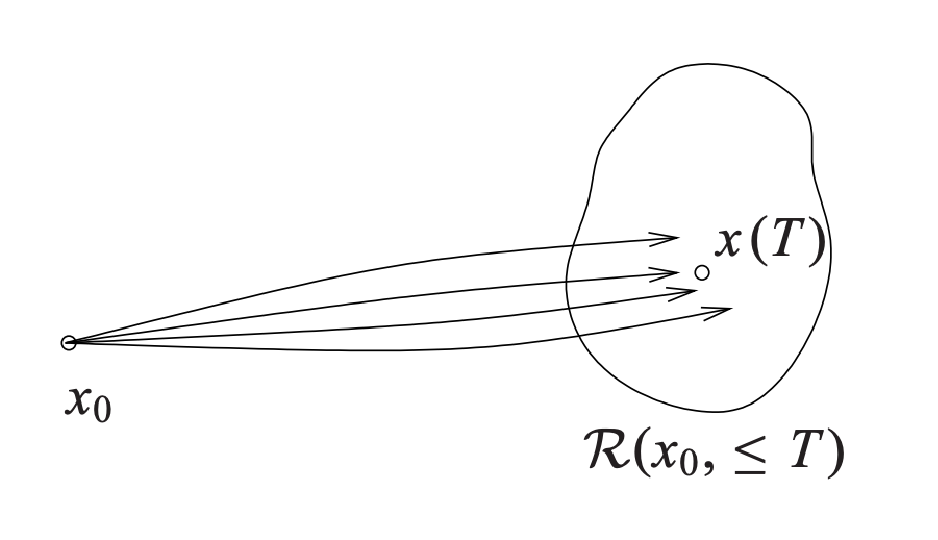
\includegraphics[width=0.5\linewidth]{figure7.1}
\\
\textbf{Figure 7.1:} The reachable set for a control system.
\end{figure}

\end{frame}	


\begin{frame}{Controllability}
	\begin{itemize}
		\item Reachability is related to a similar property called \textit{controllability}
		\item Rather than asking can we reach any state $x$ given an initial state $x_0$, controllability tackles the problem of controlling our system to a desired position $x_f$ based on a general starting position $x$
		\item These are subtly different but for linear systems, as we study in this course, reachability and controllability are equivalent
	\end{itemize}
\end{frame}


\SUBCONCEPT{Tests for reachability}

\begin{frame}{Reachability matrix}
	Define the reachability matrix
	\[W_r = \begin{bmatrix}
		B & AB & A^2 B & \cdots & A^{n-1}
	\end{bmatrix}\]
A linear system is reachable if and only if the reachability matrix $W_r$ is invertible (or equivalently, full rank)

\end{frame}

\begin{frame}{Example}
	Consider the simplified balance system (which is a model for many examples which the centre of mass is above a pivot point i.e. segway, inverted pendulum)
	\begin{align*}
		(M+m)\ddot{p}-ml\cos \theta \ddot{\theta} &= -ml\sin\theta \dot{\theta}^2+F,\\
		(J_ml^2)\ddot{\theta} -ml\cos \theta \ddot{p} &= mgl\sin \theta.
	\end{align*}
	Linearising around $(p,0,0,0)$ gives us the state space matrices
	\[ A=\begin{bmatrix}
		0 & 0 & 1 & 0\\
		0 & 0 & 0 & 1\\
		0 & m^2l^2g/\mu & 0 & 0 \\ 0& M_tmgl/\mu & 0 & 0
	\end{bmatrix}, \quad
	B = \begin{bmatrix}
		0 \\ 0 \\ Jt/\mu \\ lm/\mu
	\end{bmatrix}\]
	where $\mu=M_tJ_t-m^2l^2$, $M_t=M+m$, and $J_t=J+ml^2$
\end{frame}

\begin{frame}{Example continued}
The reachability matrix is
\begin{align*}
	W_r&= \begin{bmatrix}
		B & AB & A^2 B & A^3B
	\end{bmatrix} \\ 
	W_r &= \begin{bmatrix}
		0 & J_t/\mu & 0 & gl^3m^3/\mu^2 \\ 
		0 & lm/\mu & 0 & gl^2m^2M_t/\mu^2 \\
		J_t/\mu & 0 & gl^3m^3/\mu^2 & 0 \\
		lm/\mu & 0 & g^2l^2m^2M_t/\mu^2 & 0 
	\end{bmatrix}
\end{align*}
The determinant of this matrix is $\operatorname{det}(W_r)=-\frac{g^2l^4m^4}{\mu^6}(MJ+mJ+Mml^2)^2\neq 0$ and therefore, the reachability matrix is invertible and so the balance system is reachable!
\end{frame}

\SUBCONCEPT{Reachable canonical form}

\begin{frame}{Reachable canonical form}
\begin{itemize}
	\item Changing the coordinates and writing dynamics in this transformed coordinate system $z=Tx$ often makes calculation more convient
	\item Reachable canonical form is given by 
	\[\frac{\mathrm{d}z}{\mathrm{d}t} = \begin{bmatrix}
		-a_1 & -a_2 & -a_3 &  \cdots & -a_n	\\
		1 & 0 & & & \\
		& 1& 0 & & & \\
		& & \ddots & \ddots  & \\
		& & & 1 & 0
			\end{bmatrix}z + \begin{bmatrix}
			1 \\ 0 \\ 0 \\ \vdots \\ 0
			\end{bmatrix} u \]
			\[y=\begin{bmatrix}
				b_1 & b_2 & b_3 & \cdots & b_n
			\end{bmatrix}z + du\]
\end{itemize}
\end{frame}

\begin{frame}{Reachability canonical form}
\begin{itemize}
	\item The characteristic polynomial for a system in reachable canonical form is 
	\[\operatorname{det}(sI-A)= s^n+a_1s^{n-1}+\cdots + a_{n-1}s+a_n\]
	\item The reachability matrix in reachable canonical form is
	\[\tilde{W}_r = \begin{bmatrix}
		1 & -a_1 & a_1^2-a_2 & & \\
		0 & 1 & -a_1 & & * \\
		& & \ddots & \ddots & \\
		&  & & 1 & -a_1 \\
		& & & & 1
	\end{bmatrix}\]
	where $*$ are possible nonzero terms
	\item The transformation matrix $T$ can be found by 
	\[T=\tilde{W_r} W_r^{-1}\]
\end{itemize}
\end{frame}


\SUMMARYFRAME
\FINALE

\end{document}

  \documentclass{beamer-control}
\usepackage{beamer-control-singlefile}
\INCLUDEONLY{Stabilisation by State Feedback}
\begin{document}
\CONCEPT{Stabilisation by State Feedback}

\begin{SUMMARY}
\begin{itemize}
\item State feedback structure
\item Reachable canonical form
\item Eigenvalue assignment
\end{itemize}
\vfill References:
\begin{itemize}
\item \astrom{§7.2}
\end{itemize}
\end{SUMMARY}



\SUBCONCEPT{State feedback structure}

\begin{frame}{Controller structure}
\begin{itemize}
\item We will assume we have a system with a linear state model that has a single input for control
\item How do we design the dynamics of a system through feedback of the state
\item The goal of a feedback controller is to control the output state $y$ to a desired state given by the input $r$
\end{itemize}
\begin{figure}
	\centering
	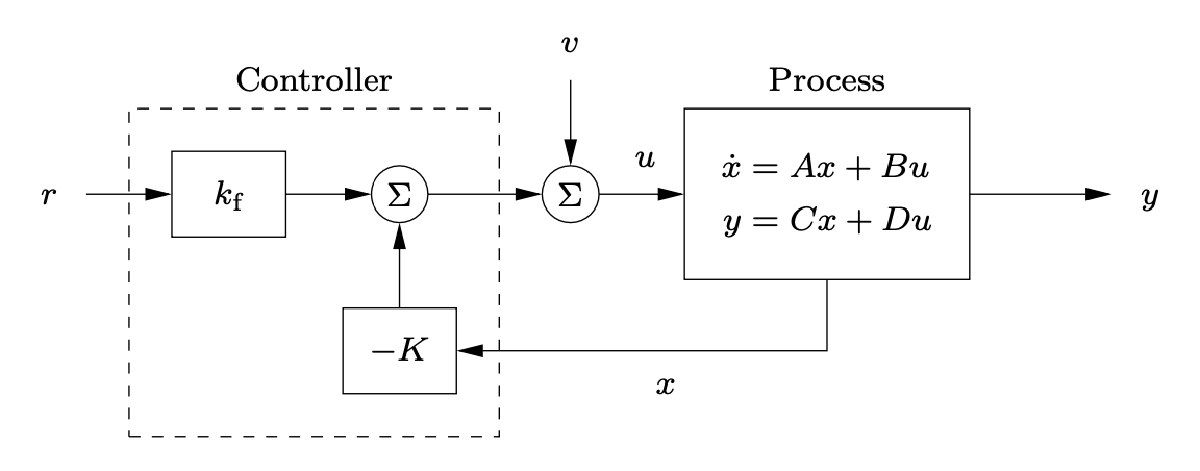
\includegraphics[width=0.8\linewidth]{figure7.5}
	\\
	\textbf{Figure 7.5:} A feedback control system with state feedback.
\end{figure}
\end{frame}


\begin{frame}{Controller structure}
	\begin{itemize}
		\item Consider a system described by
		\[ \frac{\mathrm{d} x}{\mathrm{d} t}=A x+B u, \quad y=C x+D u\]
		\item A linear control law dependent on the state $x$ and reference input $r$ can be given by 
		\[u = -Kx + k_f r\] 
		giving the closed loop state space representation 
		\[\frac{\mathrm{d} x}{\mathrm{d} t} = (A-BK)x + Bk_f r \]
	\end{itemize}
\end{frame}


\begin{frame}{Controller structure}
	\begin{itemize}
		\item We can therefore determine the characteristic polynomial of the closed loop system from our state space representation
		\item Comparing this to a \textit{desired} characteristic polynomial,
		\[p(s) = s^n + p_1 s^{n-1} + \cdots p_{n-1} s + p_n\] 
		we can design our gains $K$ and $k_f$ to meet performance specifications 
		\item Typically we want a stable equilibrium point, but maybe we care about rise time, settling time, overshoot as well 
	\end{itemize}
\end{frame}

\SUBCONCEPT{State feedback in reachable canonical form}

\begin{frame}{Reachable canonical form}
\begin{itemize}
\item Consider a system in reachable canonical form
\[\frac{\mathrm{d} z}{\mathrm{d} t}=\tilde{A} z+\tilde{B} u=\begin{bmatrix}
	-a_1 & -a_2 & -a_3 & \ldots & -a_n \\
	1 & 0 & & &  \\
	& 1 & 0 & & \\
	& & \ddots & \ddots & \\
	& & & 1 & 0
\end{bmatrix} z+\begin{bmatrix}
	1 \\
	0 \\
	0 \\
	\vdots \\
	0
\end{bmatrix} u\]
\[  y=\tilde{C} z=\begin{bmatrix}
	b_1 & b_2 & \cdots & b_n
\end{bmatrix}z \]
\item From the Reachability lecture slides, the open loop system has characteristic polynomial
\[\operatorname{det}(sI-A) = s^n+a_1s^{n-1}+\cdots + a_{n-1}s+a_n\]
\end{itemize}
\end{frame}

\begin{frame}{Reachable canonical form }
	\begin{itemize}
		\item For control law \[u=-\tilde{K}z+k_f r=-\tilde{k}_1z_1-\tilde{k}_1z_1- \cdots - \tilde{k}_nz_n+k_fr,\] the closed loop system is 
		\[  \frac{\mathrm{d} z}{\mathrm{d} t}=\begin{bmatrix}
			-a_1-\tilde{k}_1 & -a_2-\tilde{k}_2 & -a_3-\tilde{k}_3 & \ldots & -a_n-\tilde{k}_n \\
			1 & 0 & & & \\
			& 1 & 0 & & \\
			&  & \ddots & \ddots & \\
			& & & 1 & 0
		\end{bmatrix} z+\begin{bmatrix}
			k_{\mathrm{f}} \\
			0 \\
			0 \\
			\vdots \\
			0
		\end{bmatrix} r  \]
		\[y = \begin{bmatrix}
			b_1 & b_2 & \cdots & b_n
		\end{bmatrix}z\]
		\item The closed loop system has characteristic polynomial
		\begin{align*}
		\operatorname{det}(sI-A+BK) &= s^n+\left(a_1+\tilde{k}_1\right) s^{n-1}+\left(a_2+\tilde{k}_2\right) s^{n-2}\\
		&+\cdots+\left(a_{n-1}+\tilde{k}_{n-1}\right) s+a_n+\tilde{k}_n   \end{align*}
	\end{itemize}
\end{frame}


\begin{frame}{Reachable canonical form}
\begin{itemize}
	\item Therefore, we find that relating the desired characteristic polynomial to the closed loop characterisic polynomial we have
	\[\tilde{K} = \begin{bmatrix}
		p_1-a_1 & p_2-a_2 & \cdots & p_n-a_n
	\end{bmatrix}\]
	\item Further, to have zero frequency gain equal to unity we have
	\[k_f = \frac{a_n+\tilde{k}_n}{b_n}=\frac{p_n}{b_n}\]
\end{itemize}
\end{frame}



\SUBCONCEPT{Eigenvalue assignment}
\begin{frame}{Design with reachable canonical form}
This process allows us to assign the eigenvalues of the closed loop system to the eigenvalues of a desired system only if the system is reachable
\begin{enumerate}
	\item Given a linear state space model, $A$, $B$, $C$, and $D$, calculate the characteristic polynomial
	\[\operatorname{det}(sI-A) = s^n+a_1s^{n-1}+\cdots + a_{n-1}s+a_n\]
	\item Calculate gains in reachable canonical form  
	by determining  \[W_r = \begin{bmatrix}
		B & AB & A^2 B & \cdots & A^{n-1}
	\end{bmatrix},\quad \tiny{\tilde{W}_r = \begin{bmatrix}
		1 & -a_1 & a_1^2-a_2 & & \\
		0 & 1 & -a_1 & & * \\
		& & \ddots & \ddots & \\
		&  & & 1 & -a_1 \\
		& & & & 1
	\end{bmatrix}}\]
\end{enumerate}
\end{frame}

\begin{frame}{Design with reachable canonical form}
\begin{enumerate}
	\setcounter{enumi}{2}
	\item The feedback gains to give a closed loop system with unity zero frequency gain between $r$ and $y$ and characteristic polynomial
	\[p(s) = s^n+p_1 s^{n-1}+ \cdots p_{n-1}s+p_n\]
	is given by 
	\[K=\tilde{K}T = \begin{bmatrix}
		p_1-a_1 & p_2-a_2 & \cdots & p_n-a_n
	\end{bmatrix} \tilde{W}_r W_r^{-1}\]
	\[k_f = \frac{p_n}{b_n}\]
\end{enumerate}
This method is implemented in Matlab in the functions \textbf{acker} and \textbf{place}
\end{frame}

\begin{frame}{Example}
The predator-prey model is given by 
\[\frac{\mathrm{d}H}{\mathrm{d}t} = (r+u)H\left(1-\frac{H}{k} \right)-\frac{aHL}{c+H}, \quad \frac{\mathrm{d}L}{\mathrm{d}t} = \frac{baHL}{c+H}-dL\]
where the population of an ecosystem can be regulated by controlling the food supply

\begin{figure}
	\centering
	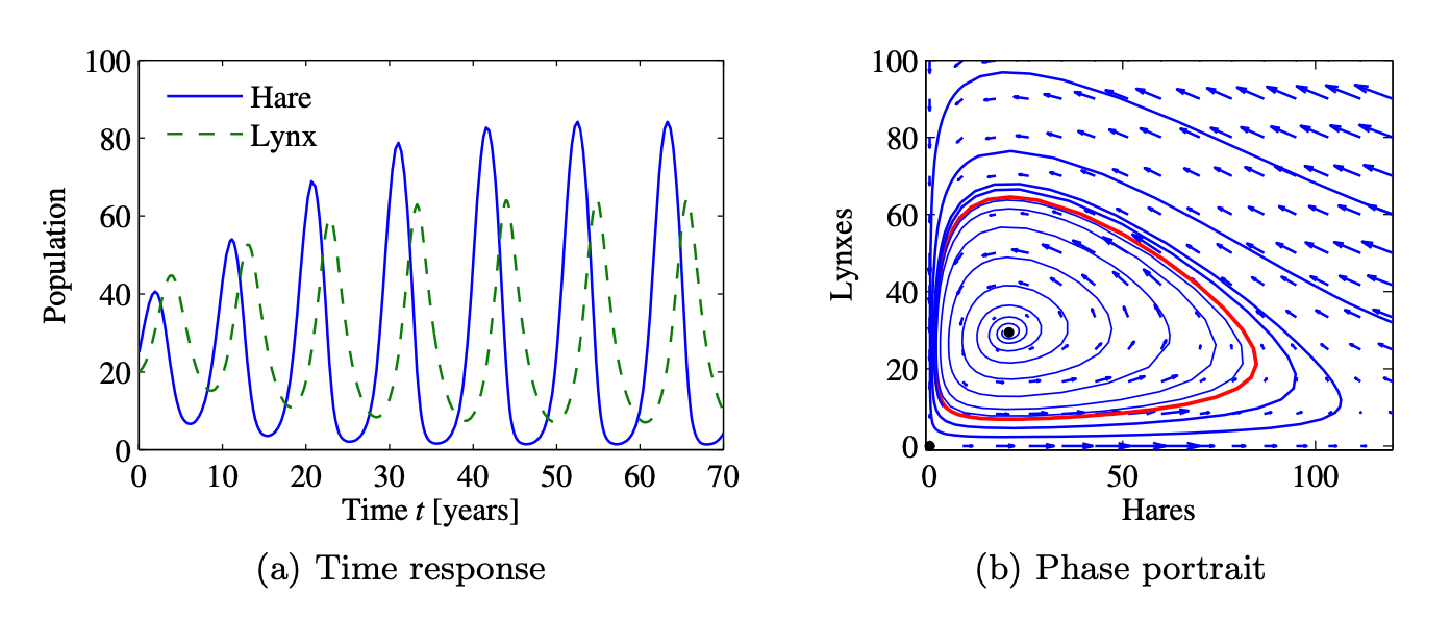
\includegraphics[width=0.8\linewidth]{figure4.20}
	\\
	\textbf{Figure 4.20:} Simulation results for the uncontrolled predator-prey system ($u=0$).
\end{figure}

\end{frame}


\begin{frame}{Example continued}
Choosing parameters $a=3.2$, $b=0.6$, $c=50$, $d=0.56$, $k=125$,  $r=1.6$, taking the growth rate for hares as the input to the system $u$ (potentially controlled by a food source for the hares), taking the number of lynxes $L$ as the output, and linearising around the equilibrium point we get 
	\[\frac{\mathrm{d}}{\mathrm{d}t}\begin{bmatrix}
		z_1 \\ z_2
	\end{bmatrix} = \begin{bmatrix}
		0.13 & -0.93 \\ 0.57 & 0
	\end{bmatrix} \begin{bmatrix}
		z_1 \\ z_2
	\end{bmatrix}  + \begin{bmatrix}
		17.2 \\ 0
	\end{bmatrix} v\]
	\[w=\begin{bmatrix}
		0& 1
	\end{bmatrix}  \begin{bmatrix}
		z_1 \\ z_2
	\end{bmatrix} \]
where $z_1=H-H_e$, $z_2=L-L_e$, and $v=u$
	
This system is reachable (by showing that the reachability matrix is full rank) and therefore we can assign the eignenvalues using state feedback

\end{frame}

\begin{frame}{Example continued}
	
	Choosing $\lambda=\begin{bmatrix}
		-0.1 & -0.2
	\end{bmatrix}$ as our desired eigenvalues, we may use the eigenvalue assignment approach to get $K=\begin{bmatrix}
		0.025 & -0.052
	\end{bmatrix}$ and $k_f=0.002$ for our gain values
	
	The resulting control law tells us how we should change the food source for the hares as a function of the current number of lynxes and hares to stabilise both populations to their equilibria
\begin{figure}
	\centering
	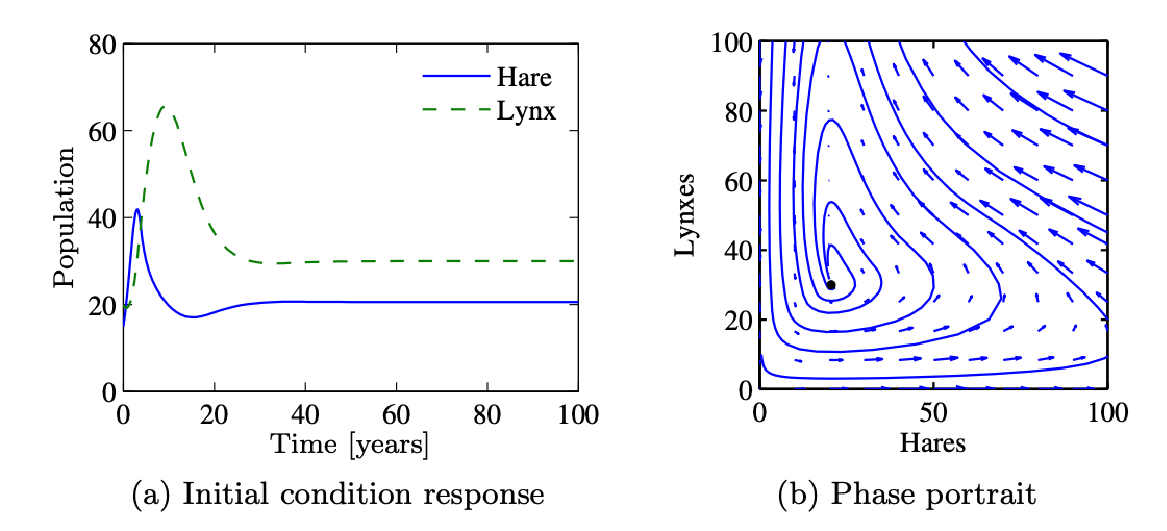
\includegraphics[width=0.8\linewidth]{figure7.7}
	\\
	\textbf{Figure 7.7:} Simulation for the controlled predator-prey system.
\end{figure}
\end{frame}


\SUMMARYFRAME
\FINALE

\end{document}

  \documentclass{beamer-control}
\usepackage{beamer-control-singlefile}
\INCLUDEONLY{State Feedback Design}
\begin{document}
\CONCEPT{State Feedback Design}

\begin{SUMMARY}
\begin{itemize}
\item Yyy
\end{itemize}
\vfill References:
\begin{itemize}
\item \astrom{Chapter Z}
\end{itemize}
\end{SUMMARY}



\SUBCONCEPT{This is a Subconcept}

\begin{frame}{This is a slide}
\begin{itemize}
\item a
\item b
\end{itemize}
\end{frame}


\SUBCONCEPT{This is another Subconcept}

\begin{frame}{This is another slide}
\begin{itemize}
\item c
\item d
\end{itemize}
\end{frame}


\SUMMARYFRAME
\FINALE

\end{document}

  \documentclass{beamer-control}
\usepackage{beamer-control-singlefile}
\INCLUDEONLY{Integral Action}
\begin{document}
\CONCEPT{Integral Action}

\begin{SUMMARY}
\begin{itemize}
\item Yyy
\end{itemize}
\vfill References:
\begin{itemize}
\item \astrom{Chapter Z}
\end{itemize}
\end{SUMMARY}



\SUBCONCEPT{This is a Subconcept}

\begin{frame}{This is a slide}
\begin{itemize}
\item a
\item b
\end{itemize}
\end{frame}


\SUBCONCEPT{This is another Subconcept}

\begin{frame}{This is another slide}
\begin{itemize}
\item c
\item d
\end{itemize}
\end{frame}


\SUMMARYFRAME
\FINALE

\end{document}

  \documentclass{beamer-control}
\usepackage{beamer-control-singlefile}
\INCLUDEONLY{Output Feedback Basics}
\begin{document}
\CONCEPT{Output Feedback Basics}

\begin{SUMMARY}
\begin{itemize}
\item Yyy
\end{itemize}
\vfill References:
\begin{itemize}
\item \astrom{Chapter Z}
\end{itemize}
\end{SUMMARY}


\SUBCONCEPT{This is a Subconcept}

\begin{frame}{This is a slide}
\begin{itemize}
\item a
\item b
\end{itemize}
\end{frame}


\SUBCONCEPT{This is another Subconcept}

\begin{frame}{This is another slide}
\begin{itemize}
\item c
\item d
\end{itemize}
\end{frame}


\SUMMARYFRAME
\FINALE

\end{document}


\TOPIC{Transfer Functions}

  \documentclass{beamer-control}
\usepackage{beamer-control-singlefile}
\INCLUDEONLY{Frequency Domain Modeling}
\begin{document}
\CONCEPT{Frequency Domain Modeling}

\begin{SUMMARY}
\begin{itemize}
\item Yyy
\end{itemize}
\vfill References:
\begin{itemize}
\item \astrom{Chapter Z}
\end{itemize}
\end{SUMMARY}



\SUBCONCEPT{This is a Subconcept}

\begin{frame}{This is a slide}
\begin{itemize}
\item a
\item b
\end{itemize}
\end{frame}


\SUBCONCEPT{This is another Subconcept}

\begin{frame}{This is another slide}
\begin{itemize}
\item c
\item d
\end{itemize}
\end{frame}


\SUMMARYFRAME
\FINALE

\end{document}

  \documentclass{beamer-control}
\usepackage{beamer-control-singlefile}
\INCLUDEONLY{Determining the Transfer Function}
\begin{document}
\CONCEPT{Determining the Transfer Function}

\begin{SUMMARY}
\begin{itemize}
\item Transmission of Exponential Signals
\item Transfer Functions for Linear Differential Equations
\begin{itemize}
\item Definition of poles and zeros
\end{itemize}
\item State Space Realisations of Transfer Functions
\end{itemize}
\vfill References:
\begin{itemize}
\item \astrom{§9.2}
\end{itemize}
\end{SUMMARY}

\SUBCONCEPT{Transmission of Exponential Signals}

\begin{frame}{The exponential signal}
\begin{itemize}
\item Define the \alert{exponential signal} $\ee^{st}$ where $s=\sigma+\ii\ww$
\end{itemize}
\begin{align}
\ee^{(\sigma+\ii\ww)t} = \ee^{\sigma t}\ee^{\ii\ww t} = \ee^{\alpha t}\left( \cos\ww t + \ii \sin \ww t \right)
\end{align}
\begin{itemize}
\item This signal allows use to representing growth/decay and/or oscillation
\end{itemize}
\end{frame}

\begin{frame}
\frametitle{Exponential signals}
\centering
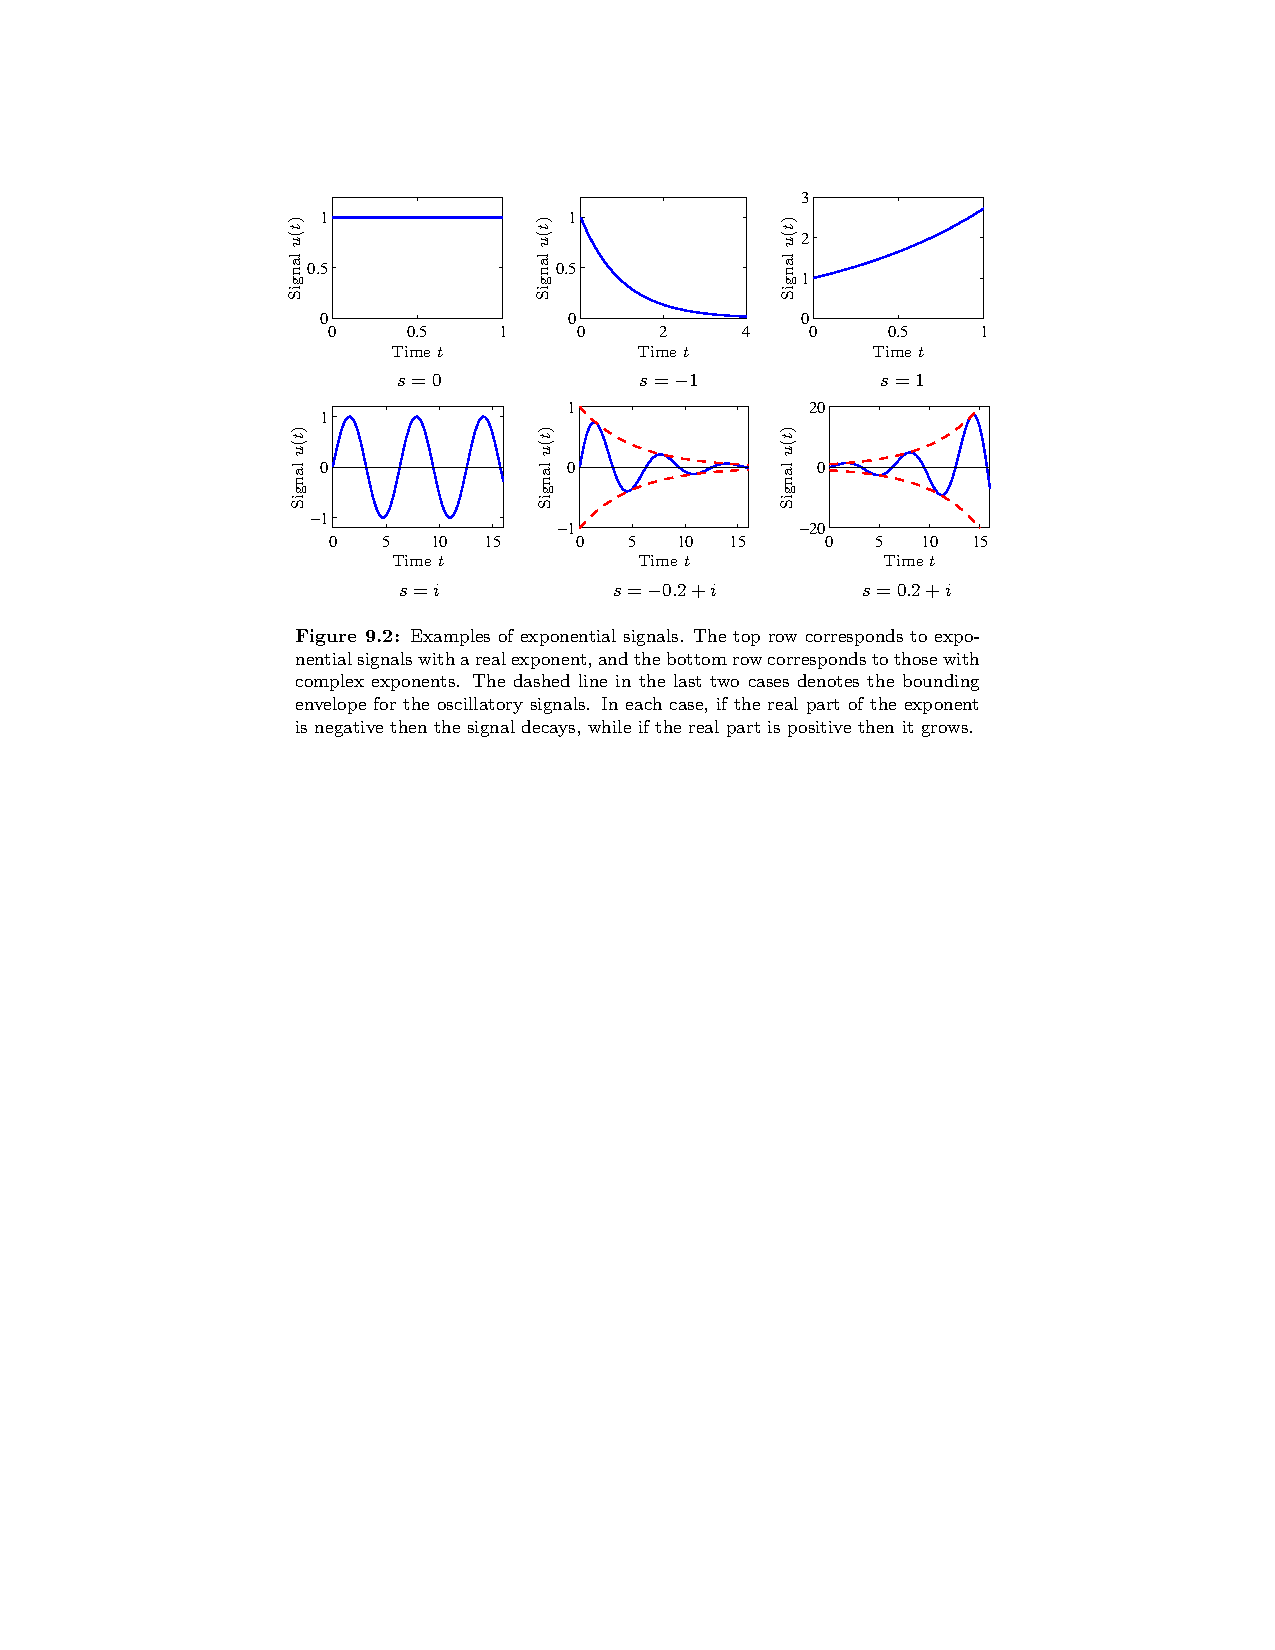
\includegraphics[width=0.8\linewidth]{figure9.2}
\end{frame}

\begin{frame}
\frametitle{Input to output}
\begin{itemize}
\item
With state space system with input $u(t)=\ee^{st}$ we can derive the state $x(t)$
\item
With the state $x(t)$ we can derive the output $y(t)$
\item
$y(t)$ consists of: (transient response terms) + \\\hfill (pure exponential response $y_p(t)$)
\item
The transfer function captures steady state output, so we define:
\end{itemize}
\begin{align}
y_p(t) &= G(s) \ee^{st} \,, \\
G(s) &= C(sI-A)\Inv B + D
\end{align}
Note: $s=\lambda_j(A)$ are special values of $s$ --- important later!
\end{frame}


\begin{frame}
\frametitle{Damped Oscillator \AMref{Example 9.1}}
We've looked previously at the damped oscillator (aka mass-spring-damper in mecheng):
\begin{align}
\Deriv{x}{t} &= \Matr{0 & \ww_0\\ -\ww_0 & -2\zz\ww_0}x+\Matr{0\\ k\ww_0}u & y&= \Matr{1 & 0} x
\end{align}
With $\zeta>0$ and input $u(t)=\ee^{s t}$:
\begin{align}
G_{yu}(s) &= C(sI-A)\Inv B = \cdots = \frac{k \ww_0^2}{s^2 + 2\zz\ww_0 s + \ww_0^2}
\end{align}
\end{frame}


\begin{frame}
\frametitle{Damped Oscillator \AMref{Example 9.1}}
For a step input, $s=0$ ($\therefore~ u(t) = \Exp{0 t} = 1$):
\begin{align}
G_{yu}(0) = \left.\frac{k \ww_0^2}{s^2 + 2\zz\ww_0 s + \ww_0^2}\right|_{s=0} = k
\end{align}
For a sinusoidal input, $u=\sin\ww t$ and there is all sorts of elegant maths which we can boil down to:
\begin{align}
y &= M \sin(\ww t + \theta) \,, \\
M &= \abs\left( G(\ii\ww) \right) \\
\theta &= \arg\left( G(\ii\ww) \right)
\end{align}
You can do this analytically, and it is very fun, but generally not needed
\end{frame}


\SUBCONCEPT{Transfer Functions for Linear Differential Equations}

\begin{frame}{Linear Differential Equations}
Consider generalised linear system with input $u$ and output $y$:
\begin{align}
\Deriv{^n y}{t^n} + a_1 \Deriv{^{n-1} y}{t^{n-1}} + \cdots + a_n y = 
b_0 \Deriv{^m u}{t^m} + b_1 \Deriv{^{m-1} u}{t^{m-1}} + \cdots + b_m u
\end{align}
As $u(t)=\Exp{s t}$ gives $y(t)=y_0 \Exp{s t}$:
\begin{math}
\Deriv{^k u}{t^k} = s^k \Exp{s t}
\end{math}
and
\begin{math}
\Deriv{^k y}{t^k} = y_0 s^k \Exp{s t} 
\end{math}
\begin{multline}
y_0 s^n \Exp{s t} + a_1 y_0 s^{n-1} \Exp{s t} + \cdots + a_n y_0 \Exp{s t} = \\
b_0 s^m \Exp{s t} + b_1 s^{m-1} \Exp{s t} + \cdots + b_m \Exp{s t}
\end{multline}
\begin{align}
a(s) y_0 \Exp{s t} &= b(s) \Exp{s t} & y(t) &= \frac{b(s)}{a(s)}\Exp{s t}
\end{align}
\end{frame}

\begin{frame}
\frametitle{Poles and zeros}
\begin{align}
G(s) = \frac{b(s)}{a(s)} = \frac
  { b_0 s^m  + b_1 s^{m-1}  + \cdots + b_m  }
  { s^n + a_1 s^{n-1} + \cdots + a_n  }
\end{align}
Define:
\begin{itemize}
\item Zeros of $G(s)$: the roots of the polynomial $b(s)$
\item Poles of $G(s)$: the roots of the polynomial $a(s)$
\end{itemize}
These poles and zeros define important properties of the transfer function

\bigskip
\begin{uncoverenv}<2->
BTW: Poles of $G(s)$ = $\lambda_j(A)$, the eigenvalues of $A$ !
\end{uncoverenv}
\end{frame}

\begin{frame}
\frametitle{Common LTI systems}
\framesubtitle{Note the time delay}

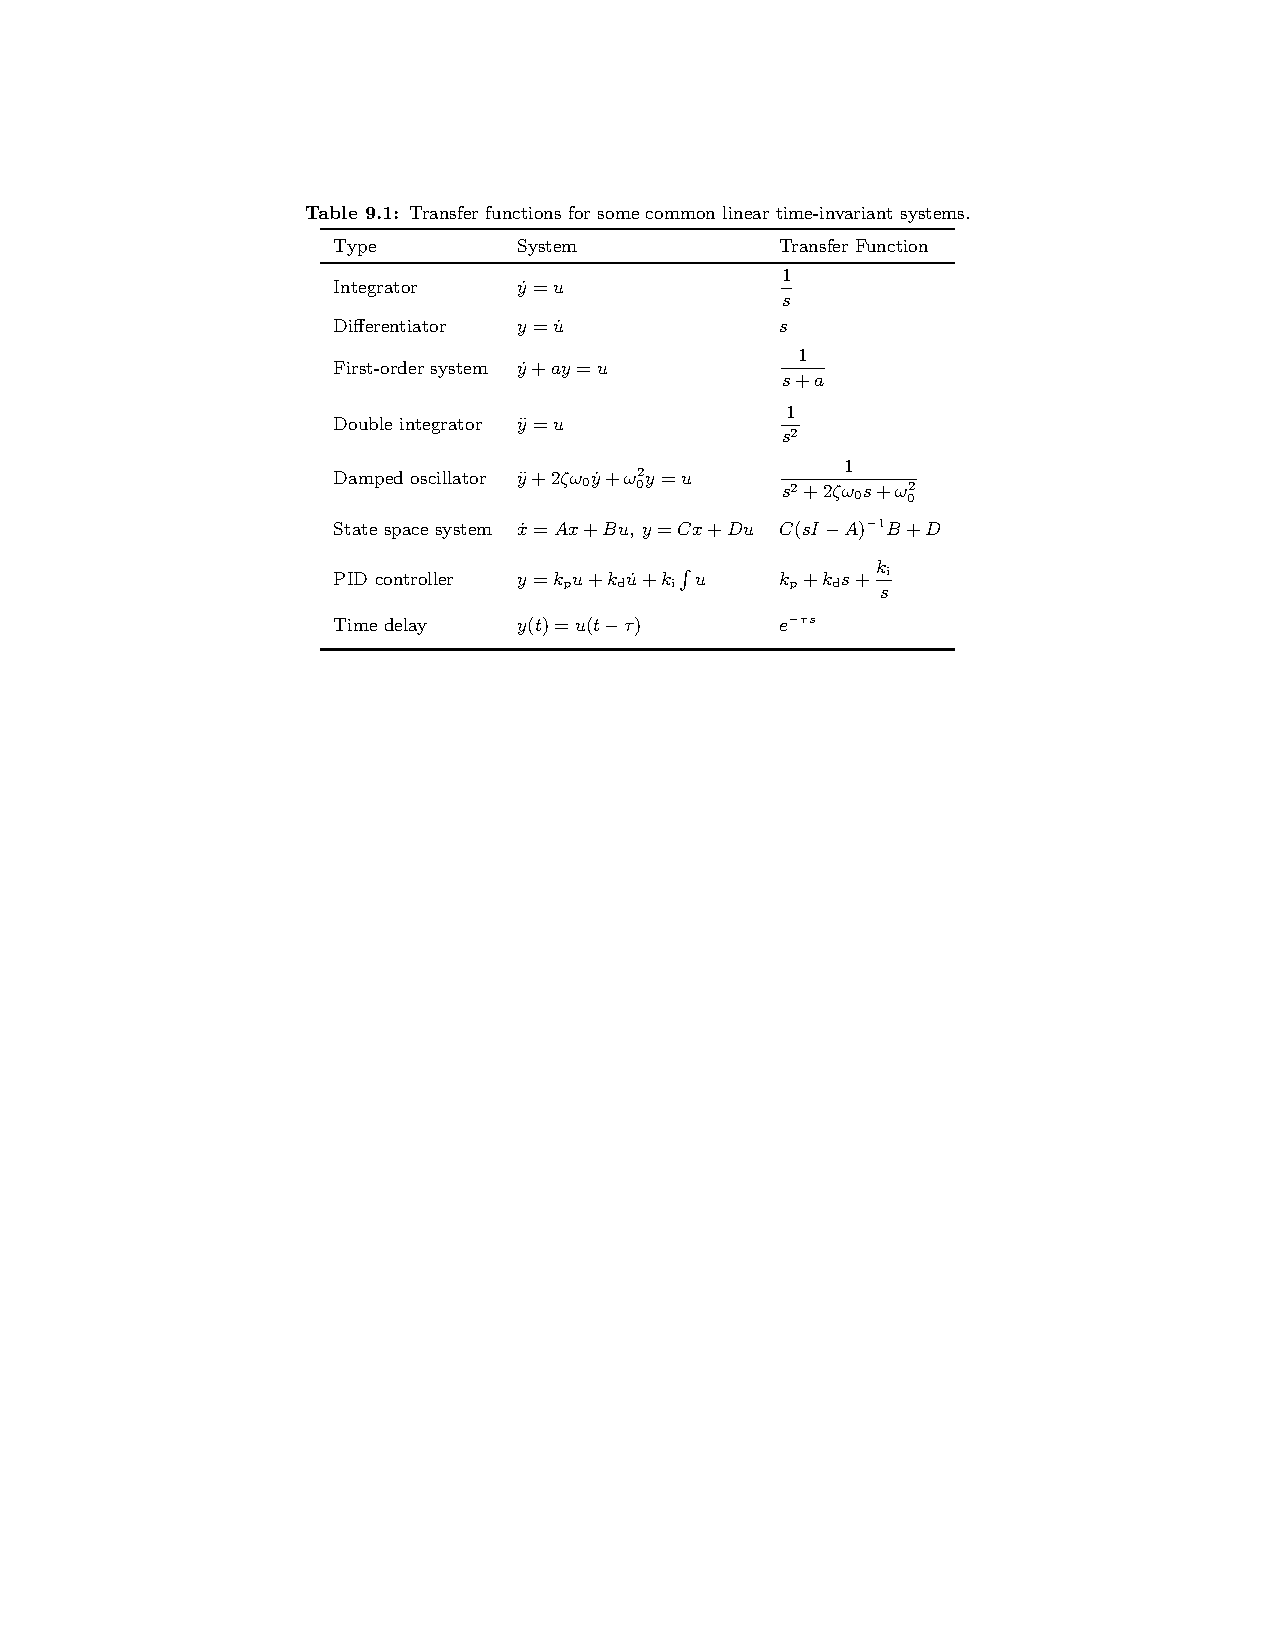
\includegraphics[height=0.8\textheight]{table9.1}


\end{frame}


\SUBCONCEPT{State Space Realisations of Transfer Functions}

\begin{frame}
\frametitle{State space vs Transfer function}
\begin{align}
\dot x &= A x + B u \,, & 
y &= Cx + Du \,, &
G(s) &= C(sI-A)\Inv B+D
\end{align}
\begin{itemize}
\item
We have seen previously that $A$, $B$, $C$, $D$ can be transformed and are not unique for a given dynamical system
\item
$G(s)$, however, is unique
\item
Textbook \AMref{Example 9.7} shows a case of \alert{pole/zero cancellation} where the transfer function ended up simpler than the state space model
\item
The \emph{minimal realisation} (\texttt{minreal()} in Matlab) is the lowest-order version of the system
\end{itemize}
\end{frame}


\SUMMARYFRAME
\FINALE

\end{document}

  \documentclass{beamer-control}
\usepackage{beamer-control-singlefile}
\INCLUDEONLY{Laplace Transforms}
\begin{document}
\CONCEPT{Laplace Transforms}

\begin{SUMMARY}
\begin{itemize}
\item Why the Laplace transform is a useful tool
\item Brief mathematical description of the Laplace transform
\item Example of solving an ODE
\item Two `theorems' which provide simple useful properties
\end{itemize}
\vfill References:
\begin{itemize}
\item \astrom{Section 9.3 `Laplace Transforms`}
\end{itemize}
\end{SUMMARY}



\begin{frame}{Reminder from TFs}
  \begin{itemize}
    \item Recall we previously analysed ODEs using a solution involving $\ee^{st}$
    \item What is $s$? Call it `complex frequency'
    \item For $s=\jj\ww$ we have sinusoidal signals with frequency $\ww$\\
          (recall $\ee^{\jj\ww t}=\cos(\ww t)+\ii \sin(\ww t)$)
    \item When we introduce a real term ($s=\sigma+\jj\ww$) this includes exponential decay (or growth)
    \item \alert{We can analyse linear systems as functions of $s$ instead of $t$}
    \item Why? Allows recipes for analytical solutions of ODEs 
  \end{itemize}
\end{frame}


\begin{frame}{Mathematical foundation}
  Close relationship between:
  \begin{itemize}
  \item Fourier series -- representing periodic signals as infinite sums of sinusoids (each with differing frequencies and amplitudes)
  \item Fourier/Laplace transforms -- converting ODEs analytically into the frequency domain 
  \item Discrete Fourier Transforms (or FFTs) -- taking measured data and numerically calculating the frequency response
  \end{itemize}
\end{frame}

\SUBCONCEPT{The Laplace transform}

\begin{frame}{Mathematically}
  Laplace transform for $s\in\mathbb{C}$:\footnote{N.B. some variances in how the limits are defined, not important here.}
  \begin{gather}
  \mathcal{L}\{f(t)\} = F(s) = \int_0^\infty f(t) e^{-st} dt
  \end{gather}
  Fourier transform for $s=\ii\omega$, with $\omega\in\mathbb{R}$:
  \begin{gather}
  \mathcal{F}\{f(t)\} = F(\omega) = \int_{-\infty}^\infty f(t) e^{-\ii\omega t} dt
  \end{gather}
  These are linear transforms:
  \begin{gather}
  \mathcal{L}\{\alert{c} f(t)\} = \alert{c}\mathcal{L}\{f(t)\} \\
  \mathcal{L}\alert{\bigl\{}f(t)\alert{+}g(t)\alert{\bigr\}} = \mathcal{L}\{f(t)\}\alert{+}\mathcal{L}\{g(t)\}
  \end{gather}
\end{frame}


\begin{frame}{This is not a course about transforms}
  Need to know (memorise):
  \begin{align}
  s &= \sigma+\jj\ww \qquad (\jj^2=-1) \\
  \mathcal{L}\bigl\{f(t)\bigr\} &= F(s) \\
  \mathcal{L}\bigl\{\frac{d}{dt}f(t)\bigr\} &= sF(s)  \\
  \mathcal{L}\bigr\{\int f(t)dt\bigr\} &= \frac{1}{s}F(s)
  \end{align}
  Note, in control, we always linearise our systems around an equilibrium and can therefore ignore initial conditions $f(0)$
\end{frame}

\begin{frame}
\frametitle{Mass-spring-damper transfer function example}
\begin{gather}
m \ddot x(t) + c \dot x(t) + kx = f(t) \\
m s^2 X(s) + c s X(s) + k X(s) = F(s) \\
\frac{X(s)}{F(s)} = \frac{1}{ms^2+cs+k}
\end{gather}
For $m=1$, $c=6$, $k=5$:
  \begin{gather}
\frac{X(s)}{F(s)} = \frac{1}{s^2+6s+5} = \frac{1}{(s+1)(s+5)}
  \end{gather}
Here we have `real poles' $s=-1, -5$: these govern the behaviour of the solution
\end{frame}

\begin{frame}
\frametitle{Tables of Laplace transforms}
  \centering
  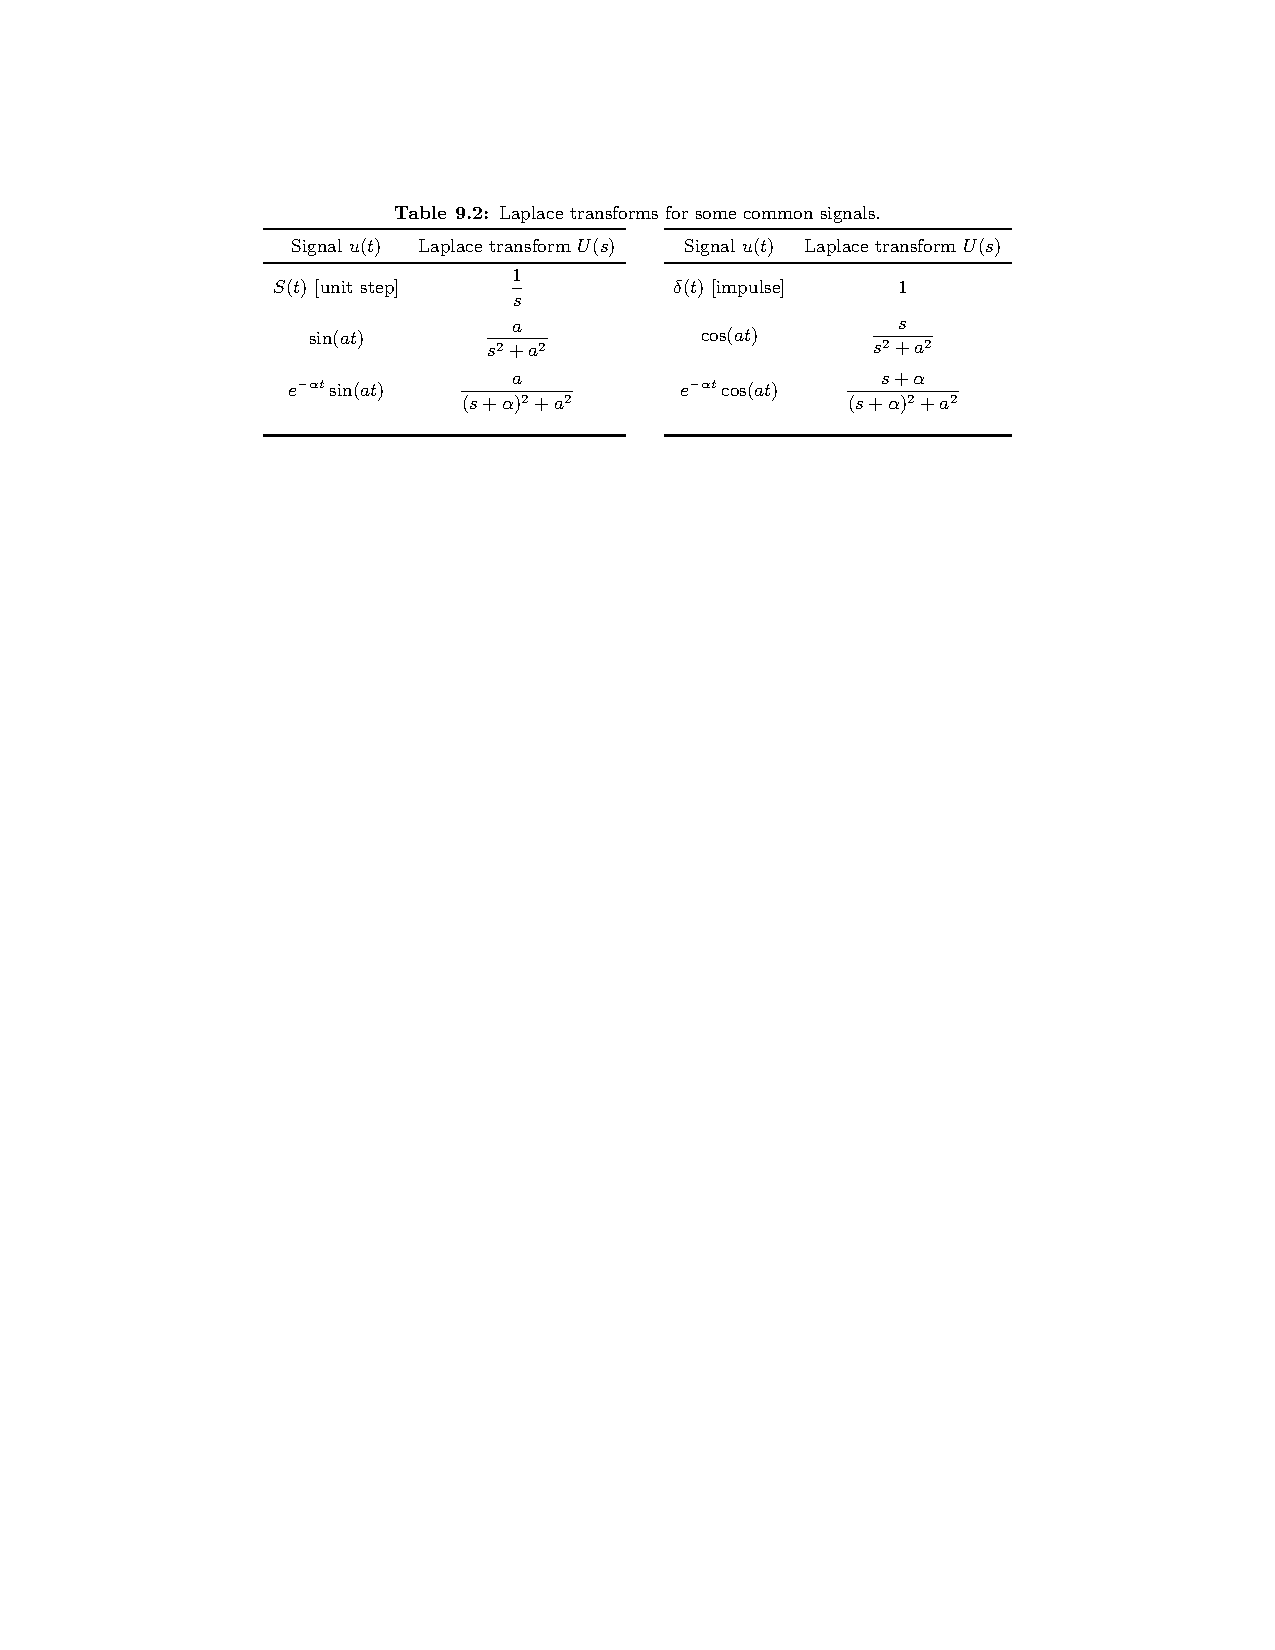
\includegraphics[width=\linewidth]{table9.2-laplace-transforms}
\end{frame}

\begin{frame}
\frametitle{Inverse Laplace transforms}
  \begin{gather}
    f(t) = \mathcal{L}^{-1}\bigl\{F(s)\bigr\} \\
    \mathcal{L}^{-1}\bigl\{b F(s) + c G(s)\bigr\} = b\mathcal{L}^{-1}\bigl\{F(s)\bigr\} + c\mathcal{L}^{-1}\bigl\{G(s)\bigr\}
  \end{gather}
  $\therefore$ A transfer function $P(s)/Q(s)$ with rational polynomials is solved using factorisation and partial fraction expansion and the result is a sum of exponential and/or sinusoid terms, e.g.:
  \begin{gather}
    \mathcal{L}^{-1}\left\{ \frac{3s+8}{s^2+2s+5} \right\} = \ee^{-t} \left( 3\cos 2t + \tfrac{5}{2}\sin 2t \right)
  \end{gather}
\end{frame}

\begin{frame}
\frametitle{Generalised second order step input example}

\begin{gather}
U(s) G(s) = \frac{1}{s}\frac{K\omega_n^2}{s^2+2\zeta\omega_ns+\omega_n^2}
\end{gather}
Assume $\zz<1$:
\begin{align}
x(t) &= \Lapl^{-1}\left\{ \frac{1}{s}\frac{K\wn^2}{s^2+2\zz\wn s+\wn^2} \right\} \\
\intertext{\em using tables of inverse Laplace transforms:}
x(t) &= K - K\frac{\exp(-\zz\wn t)}{\sqrt{1-\zz^2}}\sin\left[\wn t\sqrt{1-\zz^2}+\arccos\zz\right] \label{eq:xt2o}
\end{align}
(Now differentiate \& solve for $x'(t)=0$ to find peak response.)

\end{frame}

\SUBCONCEPT{Initial and final value theorems}

\begin{frame}
\frametitle{Initial value theorem}

\begin{gather}
\lim_{t\to0} f(t) = \lim_{s\to\infty} s F(s)
\end{gather}
Often used for transfer functions with step inputs. E.g. for system $G(s)$, step input $R(s)$, and output $U(s)$:
\begin{gather}
R(s) = \frac{1}{s} \qquad\text{\AMref{Table 9.2}}\\
u(0) = \lim_{t\to0} u(t) = \lim_{s\to\infty} s U(s) = \lim_{s\to\infty} s R(s)G(s) \\
u(0) = G(\infty)
\end{gather}
\end{frame}

\begin{frame}
\frametitle{Initial value theorem example}

Mass-spring-damper:
\begin{gather}
\frac{X(s)}{F(s)} = \frac{1}{ms^2+cs+k} \\
x(t)|_{t=0} = \lim_{s\to\infty} \frac{1}{ms^2+cs+k} = 0
\end{gather}
What does this mean? After a constant force, the response starts from zero and then builds up.

\bigskip
\QUIZ{What is the initial response to an impulse?}
\end{frame}

\begin{frame}
\frametitle{Final value theorem}

\begin{gather}
\lim_{t\to\infty} f(t) = \lim_{s\to0} s F(s)
\end{gather}
Again, very helpful when analysing step inputs. For system $G(s)$, step input $R(s)$, and output $U(s)$:
\begin{gather}
R(s) = \frac{1}{s} \qquad\text{\AMref{Table 9.2}}\\
u(\infty) = \lim_{t\to\infty} u(t) = \lim_{s\to0} s U(s) = \lim_{s\to0} s R(s)G(s) \\
u(\infty) = G(0)
\end{gather}
\end{frame}

\begin{frame}
\frametitle{Final value theorem example}

Mass-spring-damper:
\begin{gather}
\frac{X(s)}{F(s)} = \frac{1}{ms^2+cs+k} \\
x(t)|_{t=\infty} = \lim_{s\to0} \frac{1}{ms^2+cs+k} = \frac{1}{k}
\end{gather}
What does this mean? After a constant force is applied, the response starts from zero and settles to a certain value ($\frac{1}{k}$).

\bigskip
\QUIZ{What is the final response to an impulse?}
\end{frame}

\begin{frame}
\frametitle{Generalised second order system}
Recall \eqref{xt2o}:
\begin{align}
U(s)G(s) & = \frac{1}{s}\frac{K\omega_n^2}{s^2+2\zeta\omega_ns+\omega_n^2} \\
x(t) &= K - K\frac{\exp(-\zz\wn t)}{\sqrt{1-\zz^2}}\sin\left[\wn t\sqrt{1-\zz^2}+\arccos\zz\right]
\end{align}
Note:
\begin{align}
\underbrace{G(s)|_{s=0}}_{\text{DC gain}} &= K & \underbrace{x(t)|_{t\to \infty}}_{\text{SS resp.}} &= K
\end{align}
DC gain of the plant = steady state response to a step
\end{frame}

\SUMMARYFRAME
\FINALE

\end{document}

  \documentclass{beamer-control}
\usepackage{beamer-control-singlefile}
\INCLUDEONLY{Block Diagrams and Transfer Functions}
\begin{document}
\CONCEPT{Block Diagrams and Transfer Functions}

\begin{SUMMARY}
\begin{itemize}
\item Block diagrams
\item Control System Transfer Functions
\item Algebraic Loops
\end{itemize}
\vfill References:
\begin{itemize}
\item \astrom{§9.4}
\end{itemize}
\end{SUMMARY}



\SUBCONCEPT{Block diagrams}

\begin{frame}{Graphical representation of linear equations}
\framesubtitle{Aka `signal flow graphs' (more or less)}

\vfill
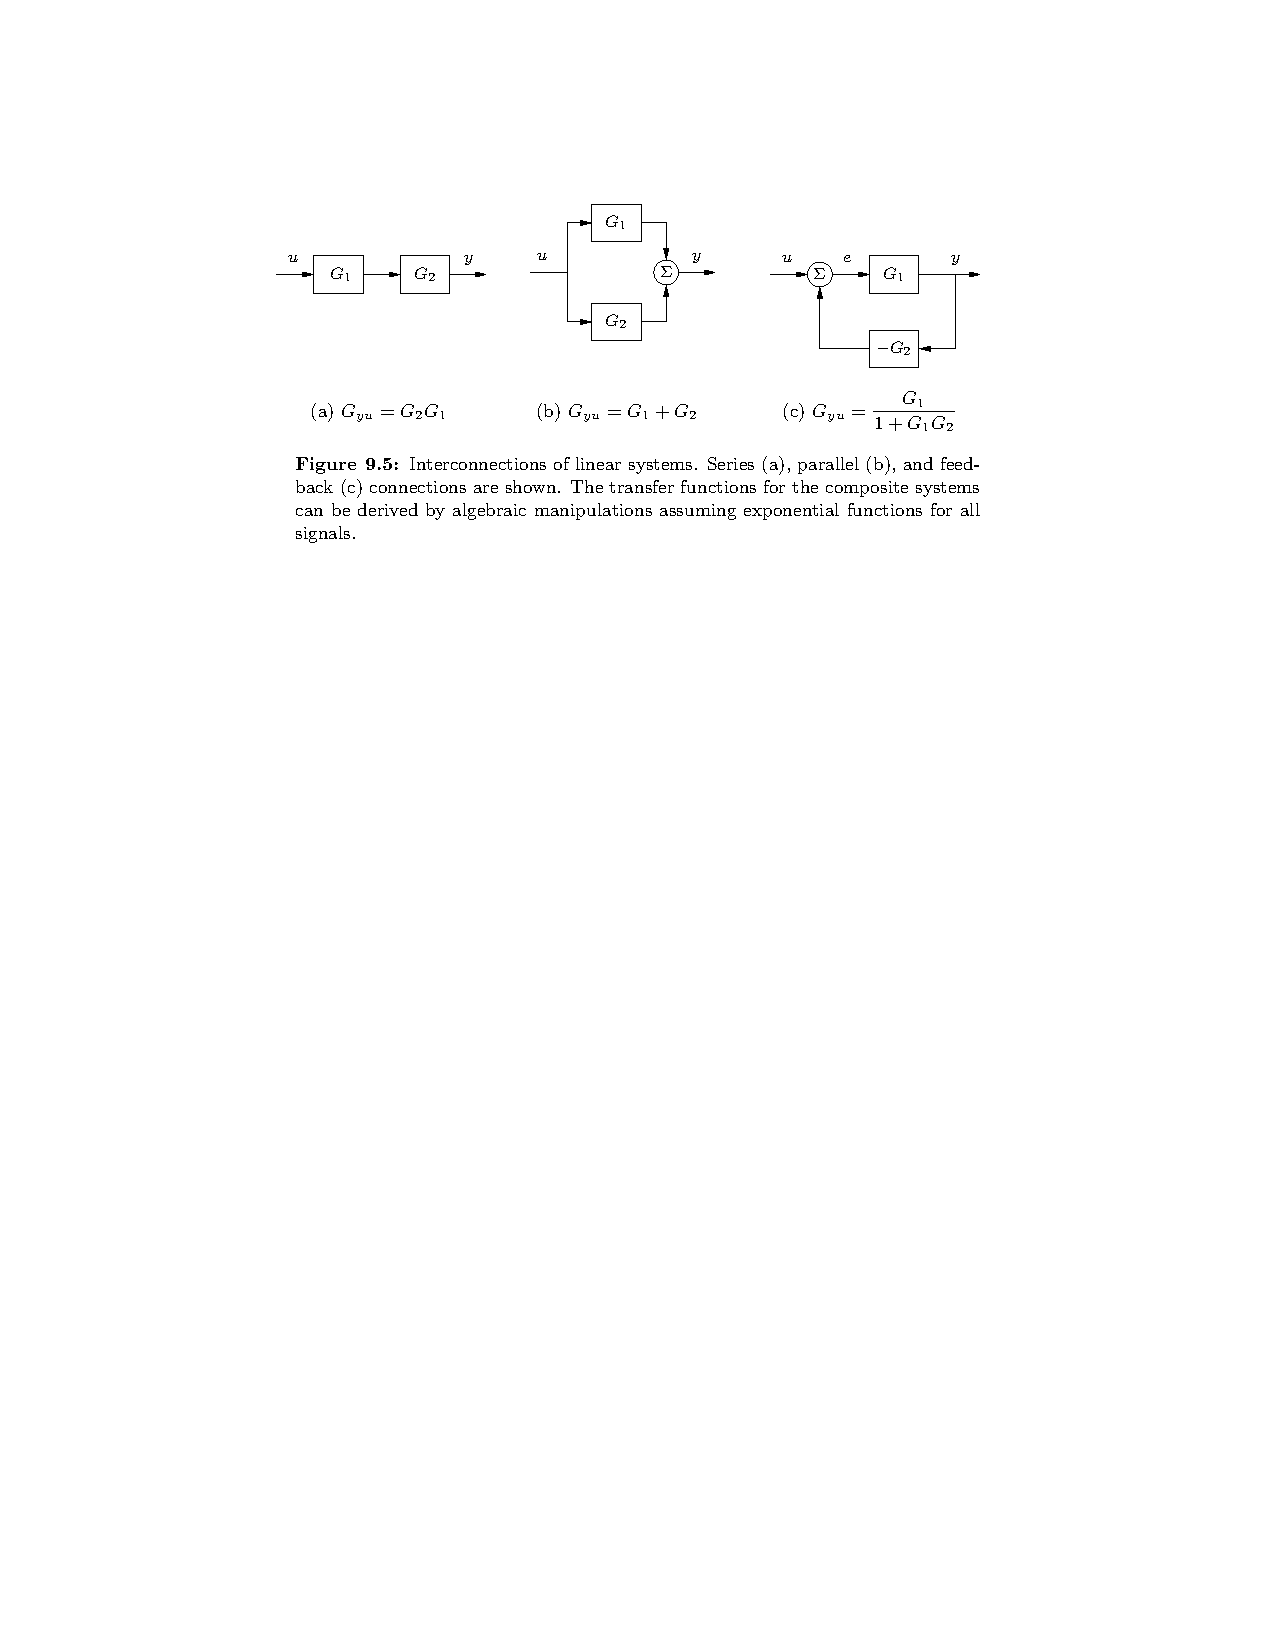
\includegraphics{figure9.5}

\end{frame}

\begin{frame}{Deriving the feedback loop}


\end{frame}

\begin{frame}{Block diagram algebra}


\end{frame}


\SUBCONCEPT{Control System Transfer Functions}

\begin{frame}{This is another slide}
\begin{itemize}
\item c
\item d
\end{itemize}
\end{frame}


\SUBCONCEPT{Algebraic Loops}

\begin{frame}{This is another slide}
\begin{itemize}
\item c
\item d
\end{itemize}
\end{frame}


\SUMMARYFRAME
\FINALE

\end{document}

  \documentclass{beamer-control}
\usepackage{beamer-control-singlefile}
\INCLUDEONLY{Zero Frequency Gain, Poles, and Zeros}
\begin{document}
\CONCEPT{Zero Frequency Gain, Poles, and Zeros}

\begin{SUMMARY}
\begin{itemize}
\item Yyy
\end{itemize}
\vfill References:
\begin{itemize}
\item \astrom{Chapter Z}
\end{itemize}
\end{SUMMARY}



\SUBCONCEPT{This is a Subconcept}

\begin{frame}{This is a slide}
\begin{itemize}
\item a
\item b
\end{itemize}
\end{frame}


\SUBCONCEPT{This is another Subconcept}

\begin{frame}{This is another slide}
\begin{itemize}
\item c
\item d
\end{itemize}
\end{frame}


\SUMMARYFRAME
\FINALE

\end{document}

  \documentclass{beamer-control}
\usepackage{beamer-control-singlefile}
\INCLUDEONLY{The Bode Plot}
\begin{document}
\CONCEPT{The Bode Plot}

\begin{SUMMARY}
\begin{itemize}
\item Sketching and Interpreting Bode Plots
\item Poles and Zeros in the Right Half-Plane
\item Time Delays
\item System Insights from the Bode Plot
\item Determining Transfer Functions Experimentally
\end{itemize}
\vfill References:
\begin{itemize}
\item \astrom{§9.6}
\end{itemize}
\end{SUMMARY}


\begin{frame}
\frametitle{Introduction}
The \alert{frequency response} of a system is computed from its transfer function with $s=\ii\ww$, which corresponds to an input of:
\begin{align}
u(t) = \Exp{\ii\ww t} = \cos \ww t + \ii \sin \ww t
\end{align}
We have seen the resulting output is
\begin{align}
y(t) = G(\ii\ww)\Exp{\ii\ww t} = M\cos(\ww t+\theta) + \ii M \sin(\ww t + \theta)
\end{align}
which use the gain $M$ and phase $\theta$ of $G$ defined as:
\begin{align}
M &= \abs (G(\ii\ww)) & \theta &= \arg( G(\ii\ww)) = \arctan \frac{\Imag G(\ii\ww)}{\Real G(\ii\ww)}
\end{align}
We can visualise $M$ and $\theta$ versus frequency --- the Bode Plot
\end{frame}

\begin{frame}{Calculating the FR analytically}
  \begin{itemize}
    \item  Start with transfer function $F(s)$\\ (mathematically $F(s)\colon\mathbb{C}\to\mathbb{C}$)
    \item  Substitute $s=\jj\ww$ \qquad --- n.b.\ real frequencies only
    \item  (If by hand, separate $F(\ww)$ into real and complex components)
    \item  Create a vector of frequencies $\ww\in\{\omega_0,\omega_1,\omega_2,\dots\}$
    \item  Calculate vector of responses $\bigl\{F(\omega_0),F(\omega_1),F(\omega_2),\dots\bigr\}$
  \end{itemize}
\end{frame}

\begin{frame}{Example}
  \begin{align*}
  G &= \frac{10}{s+5}
    = \frac{10}{5+\jj\ww}
     = \frac{10(5-\jj\ww)}{(5+\jj\ww)(5-\jj\ww)}
     = \frac{50}{25+\ww^2} + \jj\frac{-10\ww}{25+\ww^2}
  \end{align*}
  \bigskip
  \begin{align*}
  \Real(G(\ww)) & = \frac{50}{25+\ww^2} &
  \lvert G(\ww)\rvert & = \frac{\sqrt{2500+100\ww^2}}{25+\omega^2} \\
  \Imag(G(\ww)) & = \frac{-10\ww}{25+\ww^2} &
  \measuredangle G(\ww) & = \arctan(-10\ww/50)
  \end{align*}
\end{frame}

\begin{frame}
\frametitle{Example Bode Plot}
\centering
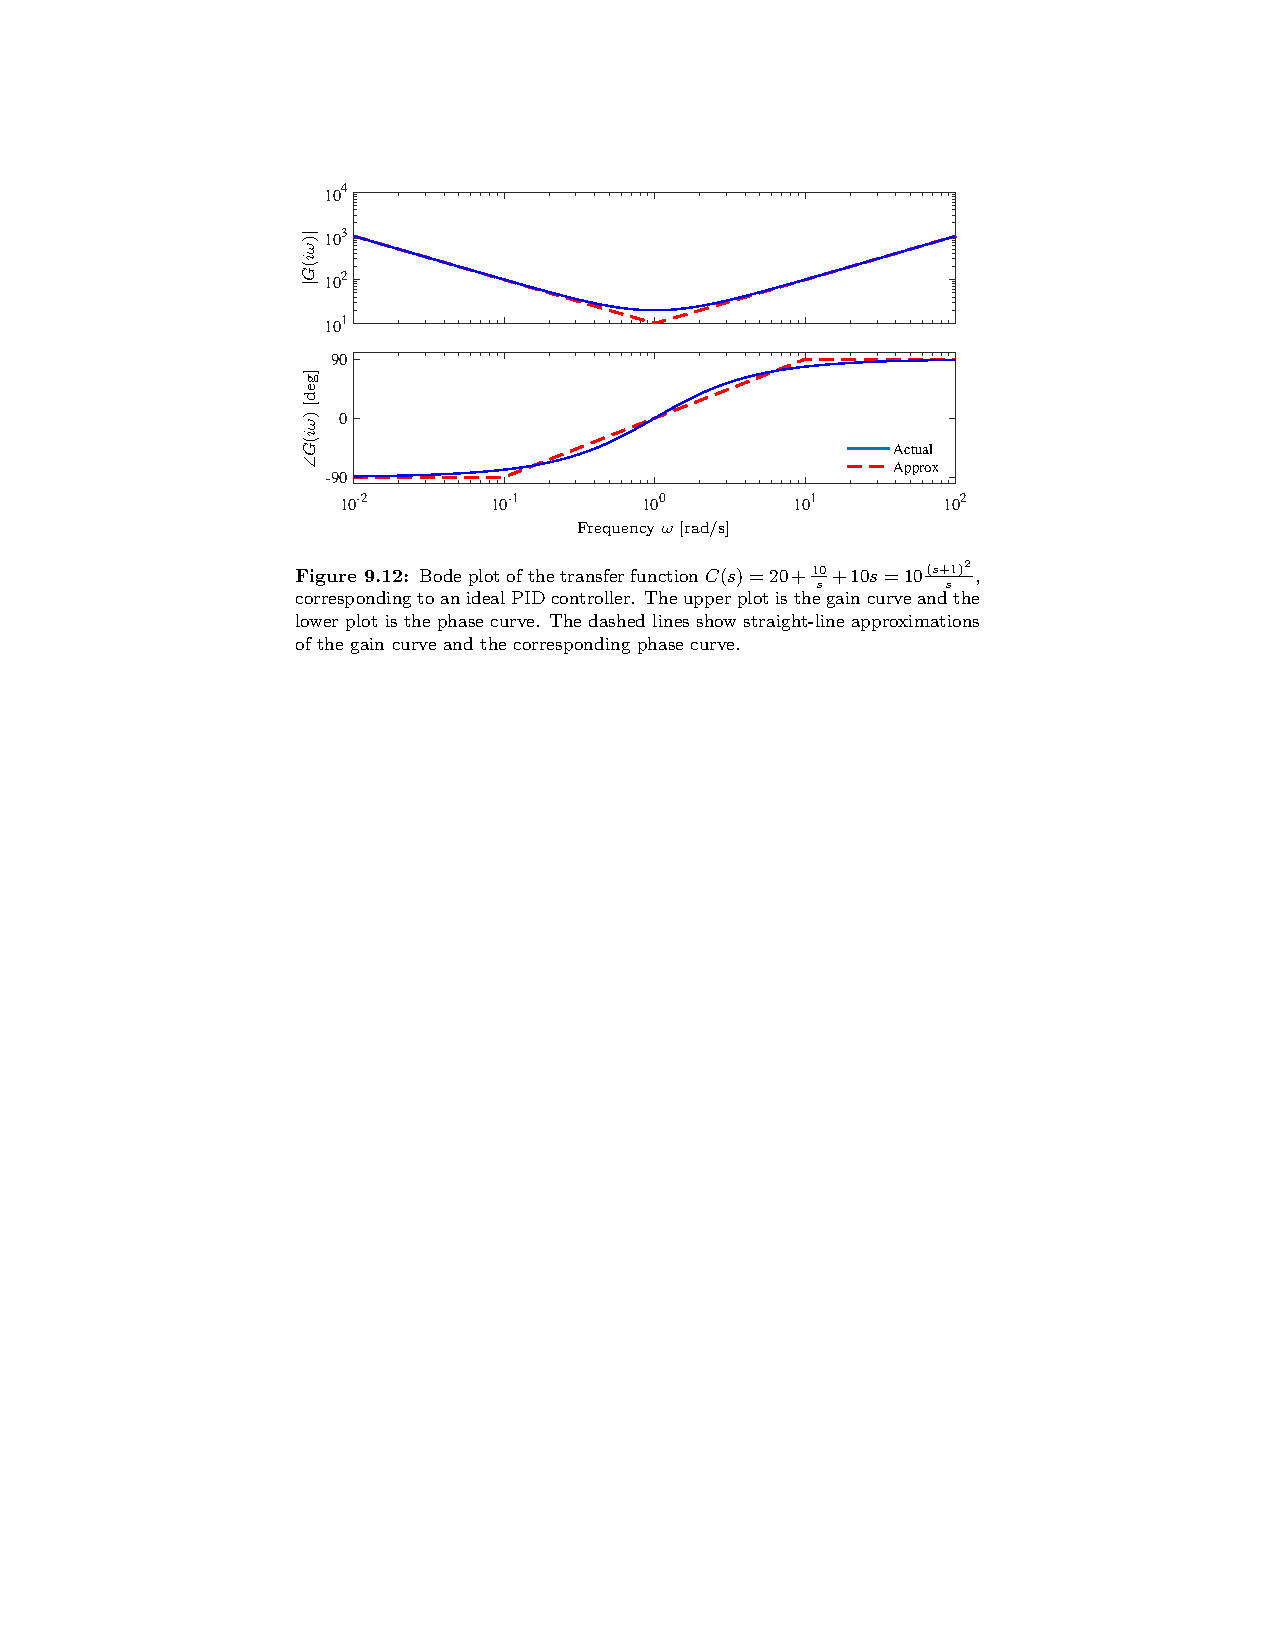
\includegraphics[width=0.8\linewidth]{figure9.12}

\end{frame}

\SUBCONCEPT{Sketching and Interpreting Bode Plots}

\begin{frame}{Canonical Bode Plots --- integrator and differentiator}
\centering
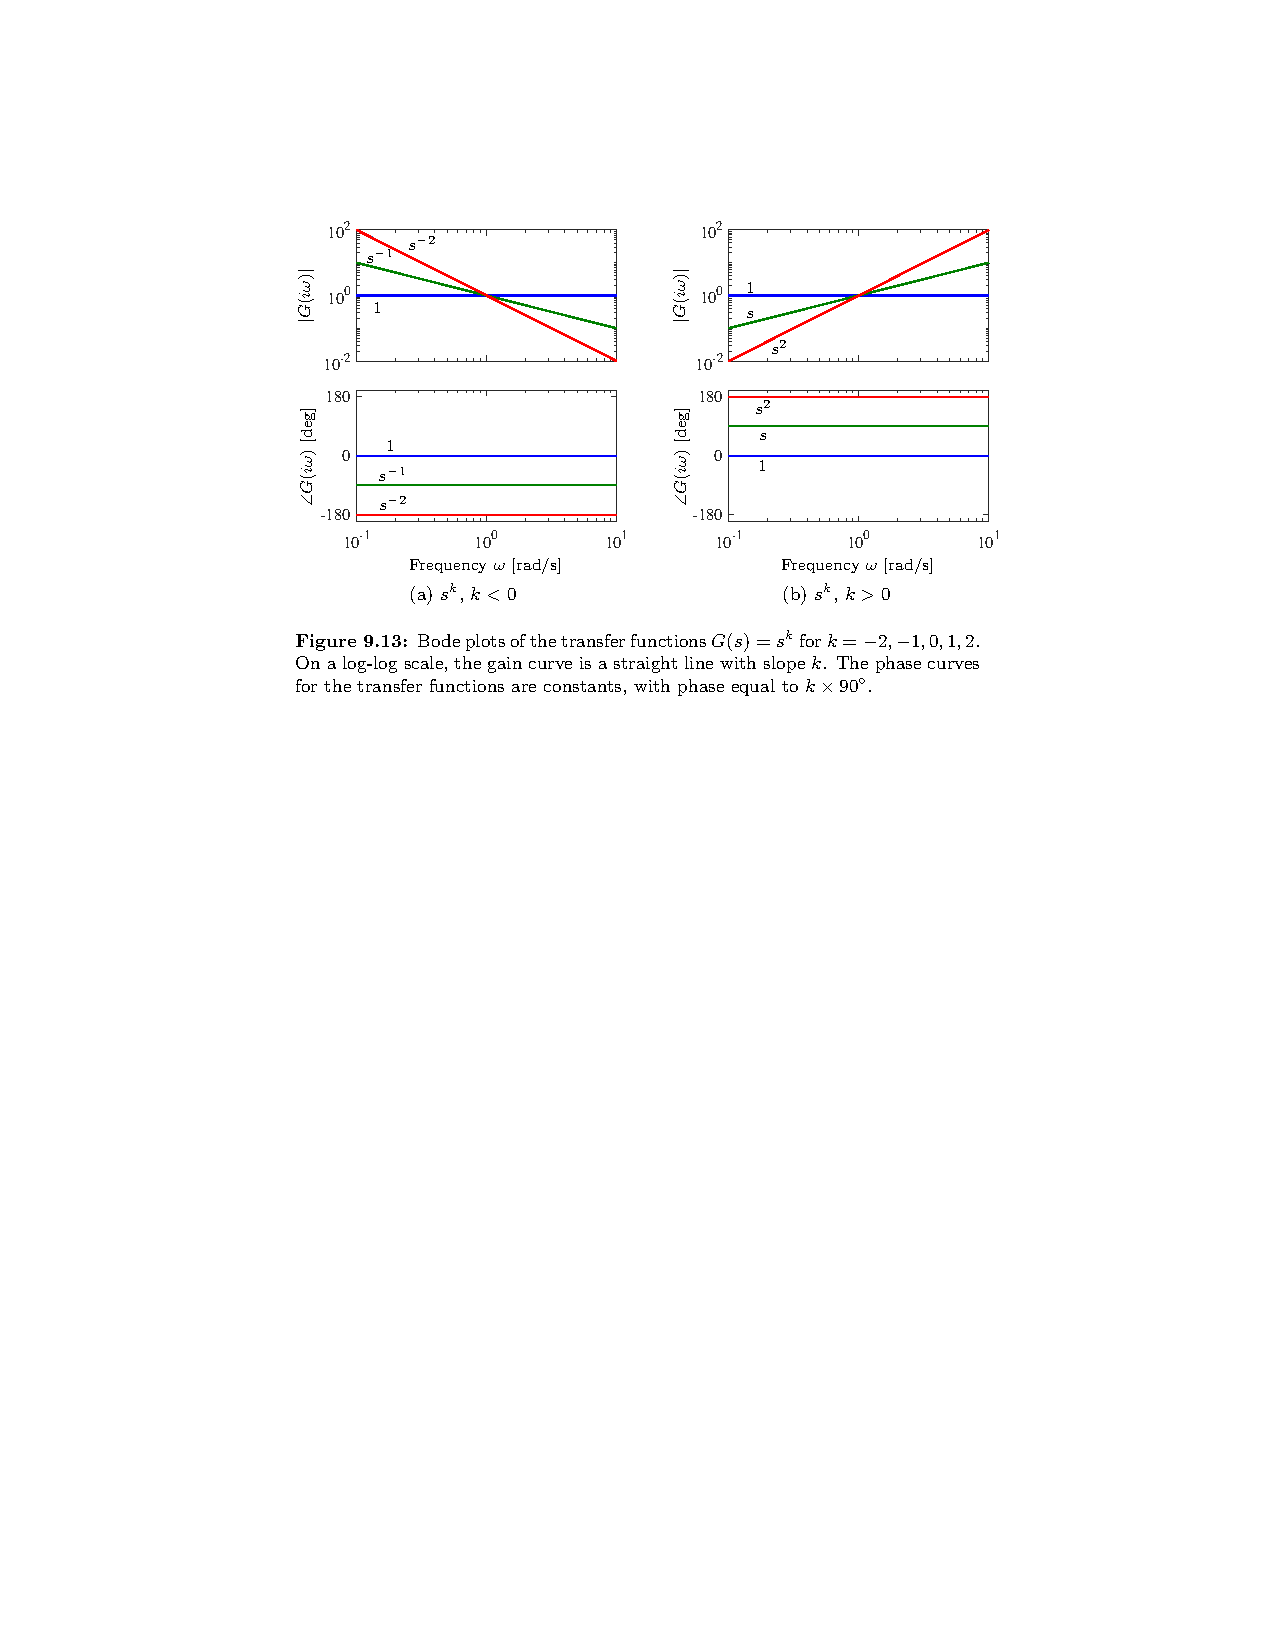
\includegraphics[height=0.8\textheight]{figure9.13}

\end{frame}

\begin{frame}{Canonical Bode Plots --- first order and second order}
\centering
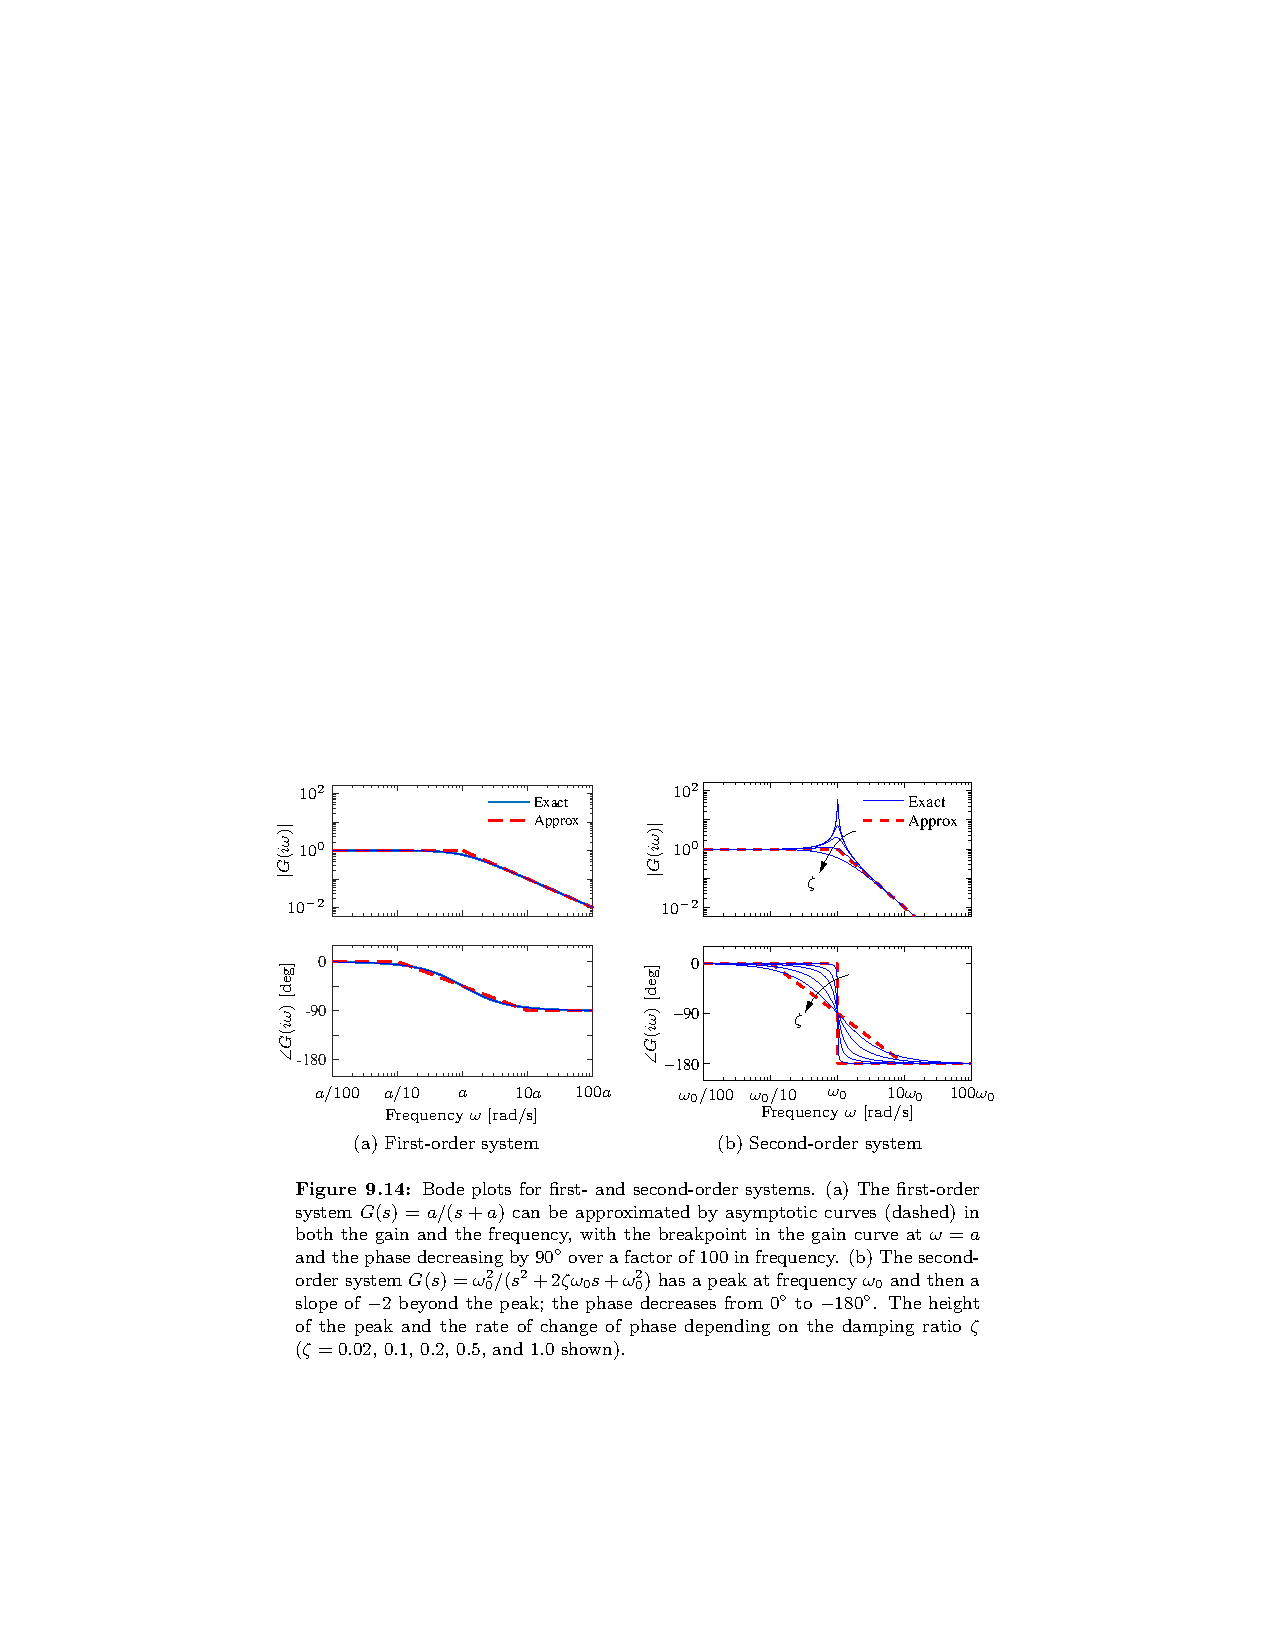
\includegraphics[height=0.8\textheight]{figure9.14}

\end{frame}

\begin{frame}{Example Bode Plot --- 1 zero, 3 pole system}
\centering
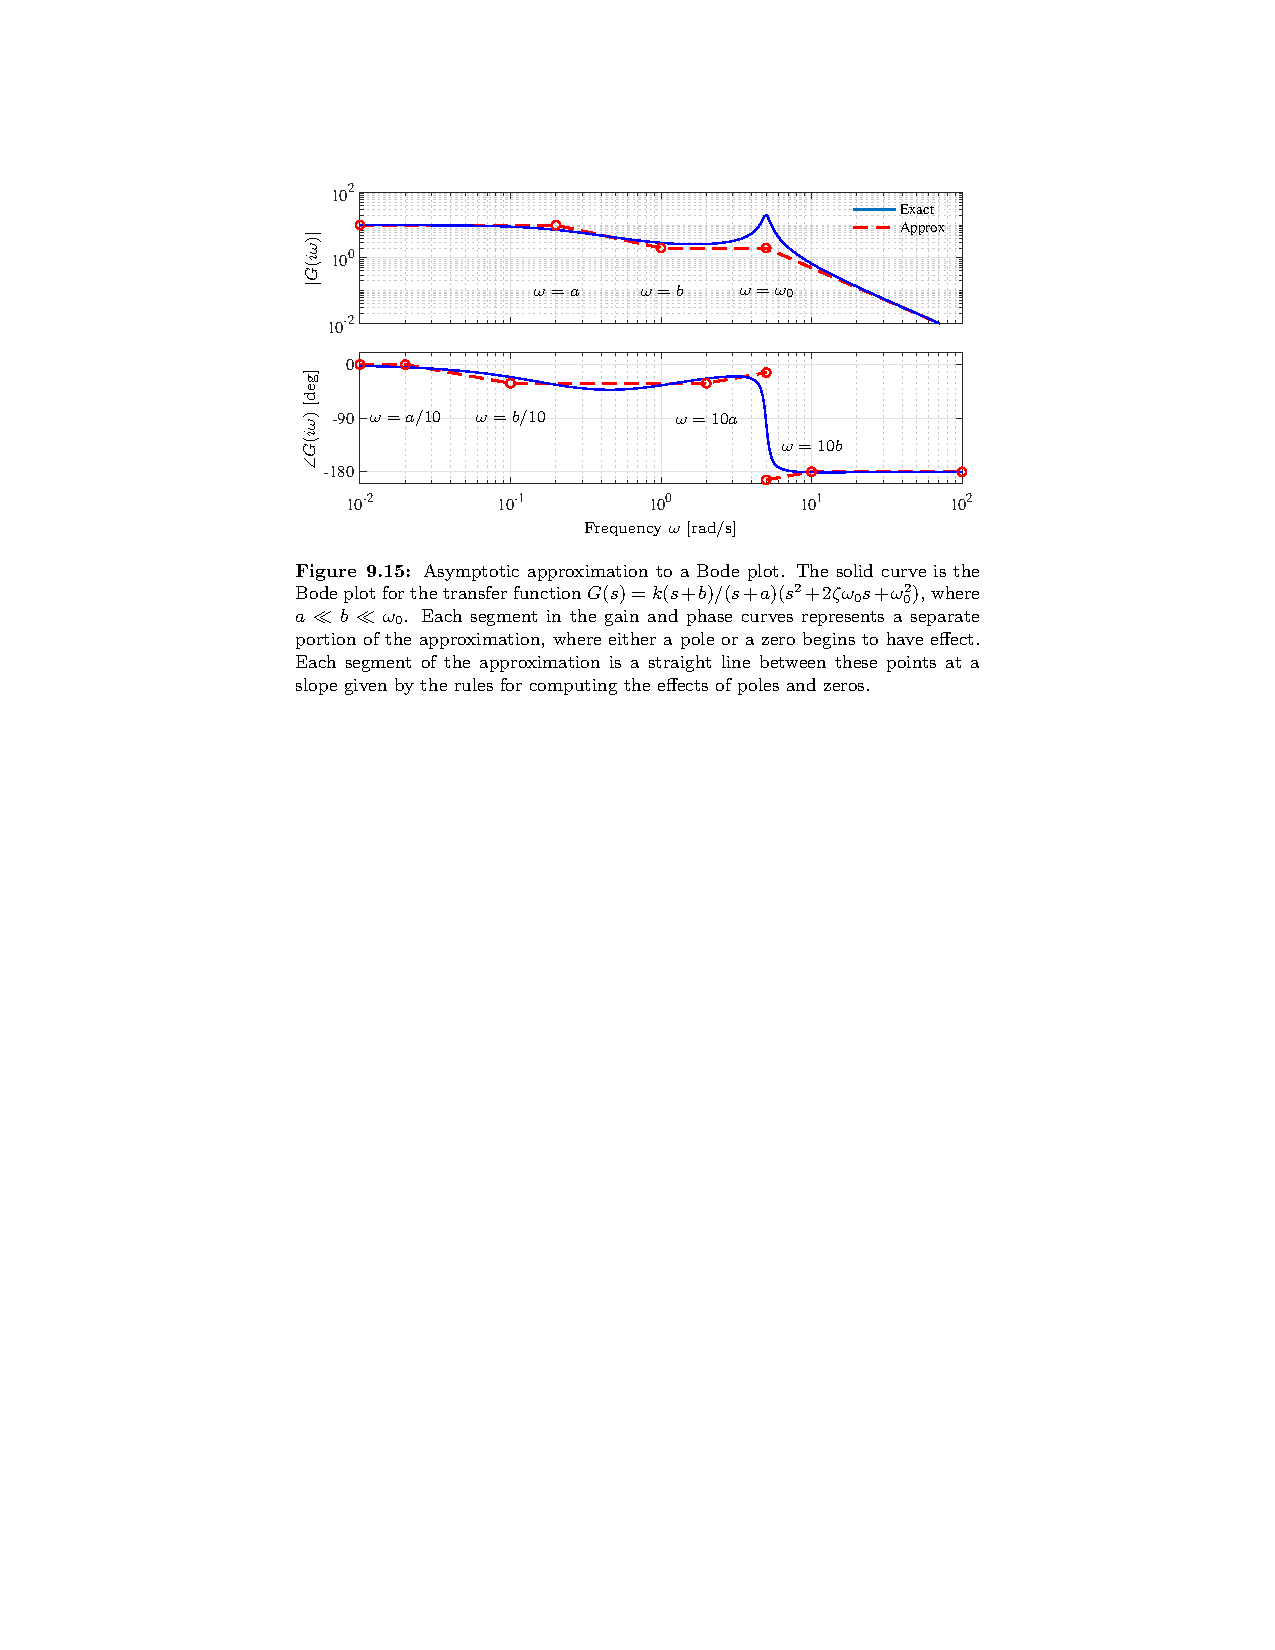
\includegraphics[height=0.8\textheight]{figure9.15}

\end{frame}




\begin{frame}
\begin{columns}
\column{0.4\linewidth}
\[
  GH = \frac{100(s+1)}{(s+10)(s+100)}
\]
\bigskip
\emph{In Matlab:}

\includematlab{bode1.m}{bode2}

\bigskip
{\tiny Actually the plot on the right is done a little more carefully.\par}

\column{0.6\linewidth}
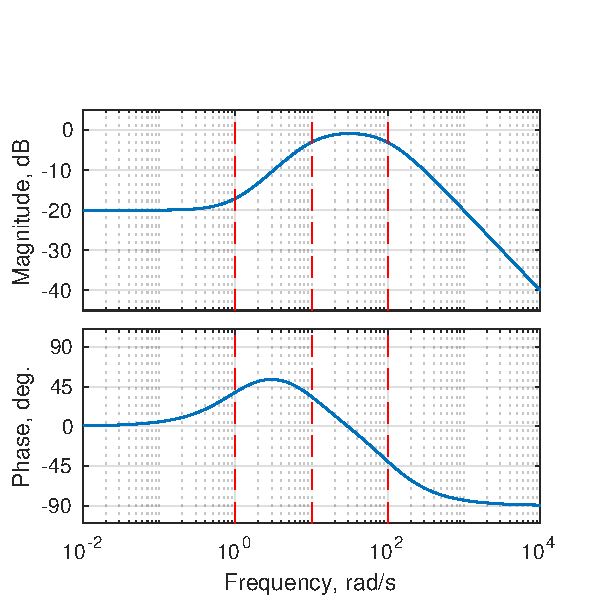
\includegraphics[width=\linewidth,clip,trim=0 0 0 30]{bode1.pdf}
\end{columns}
\end{frame}


\begin{frame}{Summary of rules}
  Magnitude:
  \begin{itemize}
    \item  Starts at magnitude of DC gain
    \item  Start with `flat' slope of \SI{0}{dB/dec}
    \item  One pole: add $-\SI{20}{dB/dec}$ slope
    \item  One zero: add $+\SI{20}{dB/dec}$ slope
  \end{itemize}
  Phase:
  \begin{itemize}
    \item  Start at \ang{0}
    \item  One pole: transition through $-\ang{90}$ (over one decade)
    \item  One zero: transition through $+\ang{90}$ (over one decade)
  \end{itemize}
  Important point:
  \begin{itemize}
    \item  Integrator is a pole at $s=0$
    \item  Differentiator is a zero at $s=0$
    \item  Same rules apply
  \end{itemize}
\end{frame}


\begin{frame}{More on phase limits}{For stable plants with +ve DC gain}
\begin{columns}[t]
\small
\column{0.5\linewidth}
Low frequency phase limit:
\[
\theta_0 = -\ang{90}\times(N_I-N_D)
\]
where
\begin{itemize}
\item $N_I =$ number of integrators
\item $N_D =$ number of differentiators
\end{itemize}

\column{0.5\linewidth}
High frequency phase limit:
\[
\theta_\infty = -\ang{90}\times(N_P-N_Z)
\]
where
\begin{itemize}
\item $N_P =$ number of poles\\ (incl.\ integrators)
\item $N_Z =$ number of zeros\\ (incl.\ differentiators)
\end{itemize}
$n_{pe} = (N_P-N_Z)$ is used often and termed the `poles excess'


\end{columns}
\end{frame}


\SUBCONCEPT{Poles and Zeros in the Right Half-Plane}

\begin{frame}
\frametitle{Non-minimum phase zeros}
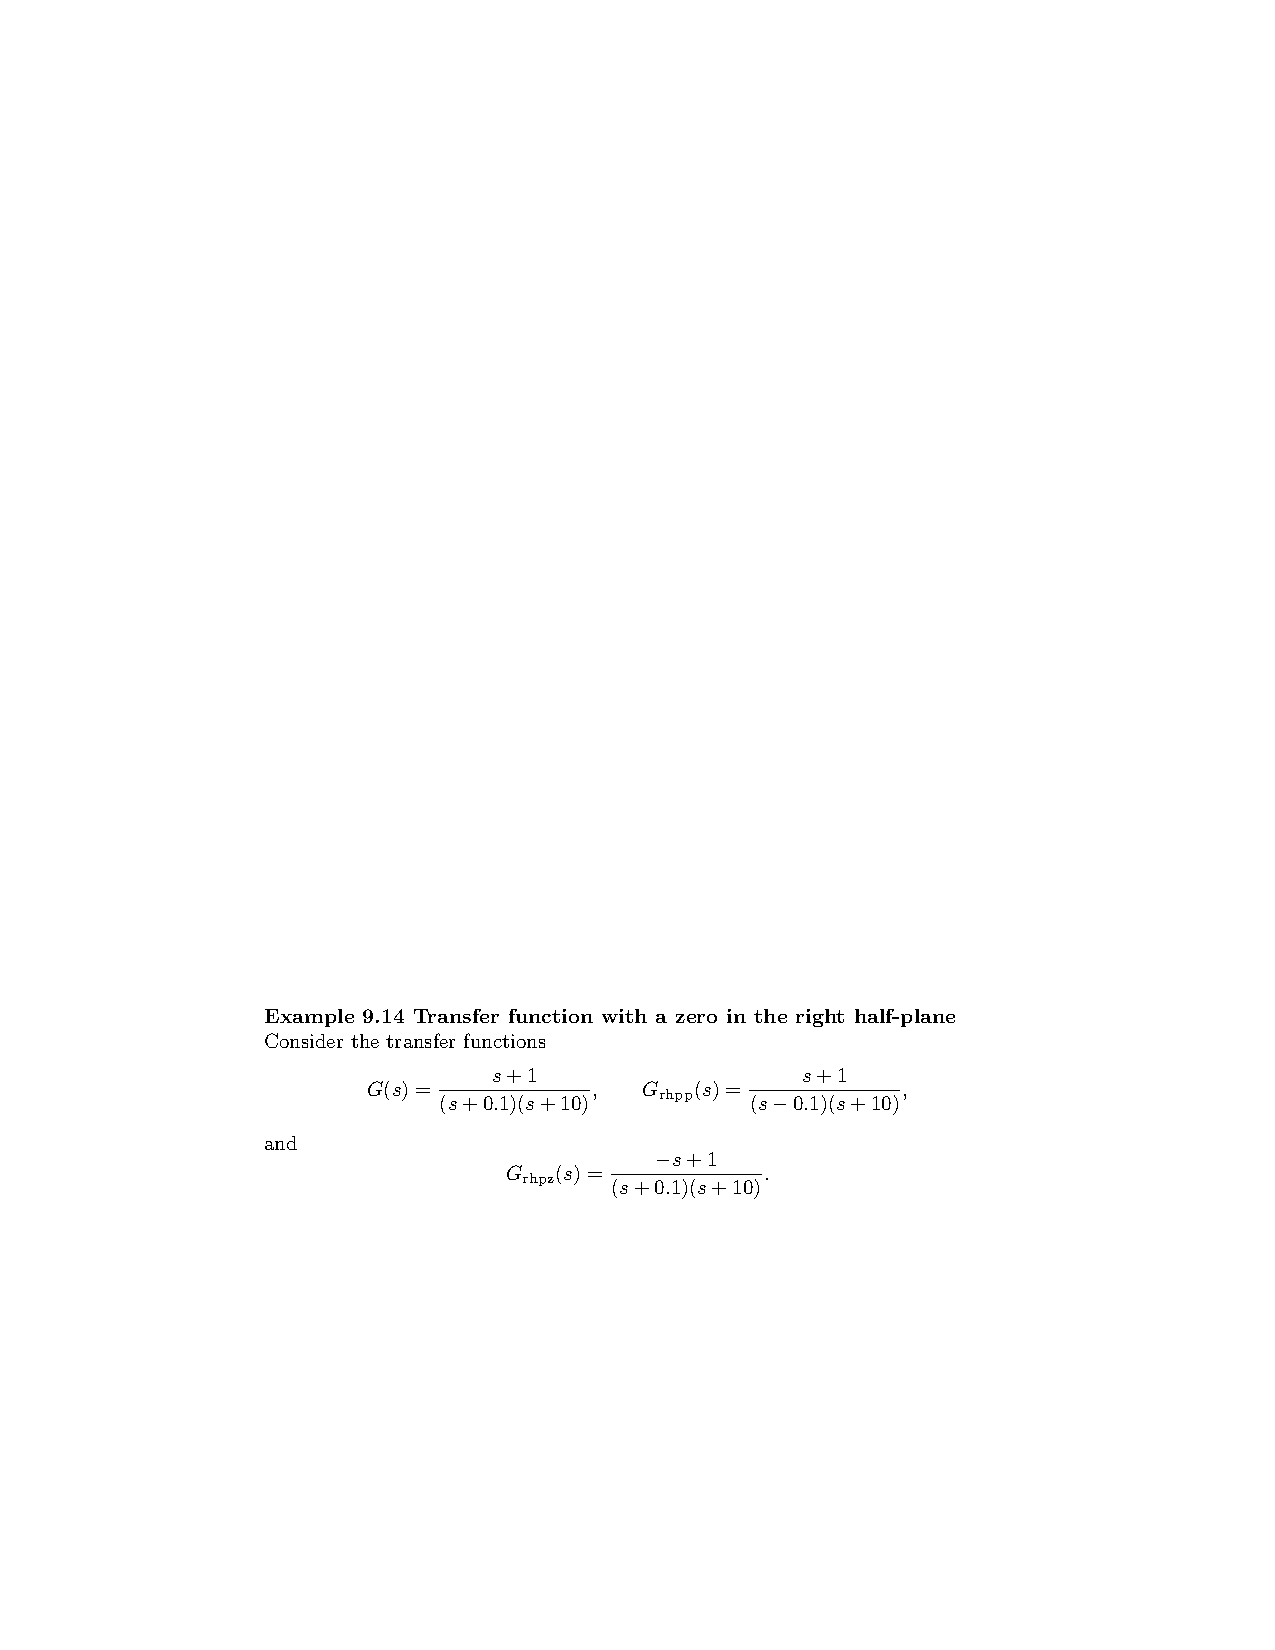
\includegraphics[width=0.8\linewidth]{example9.14}

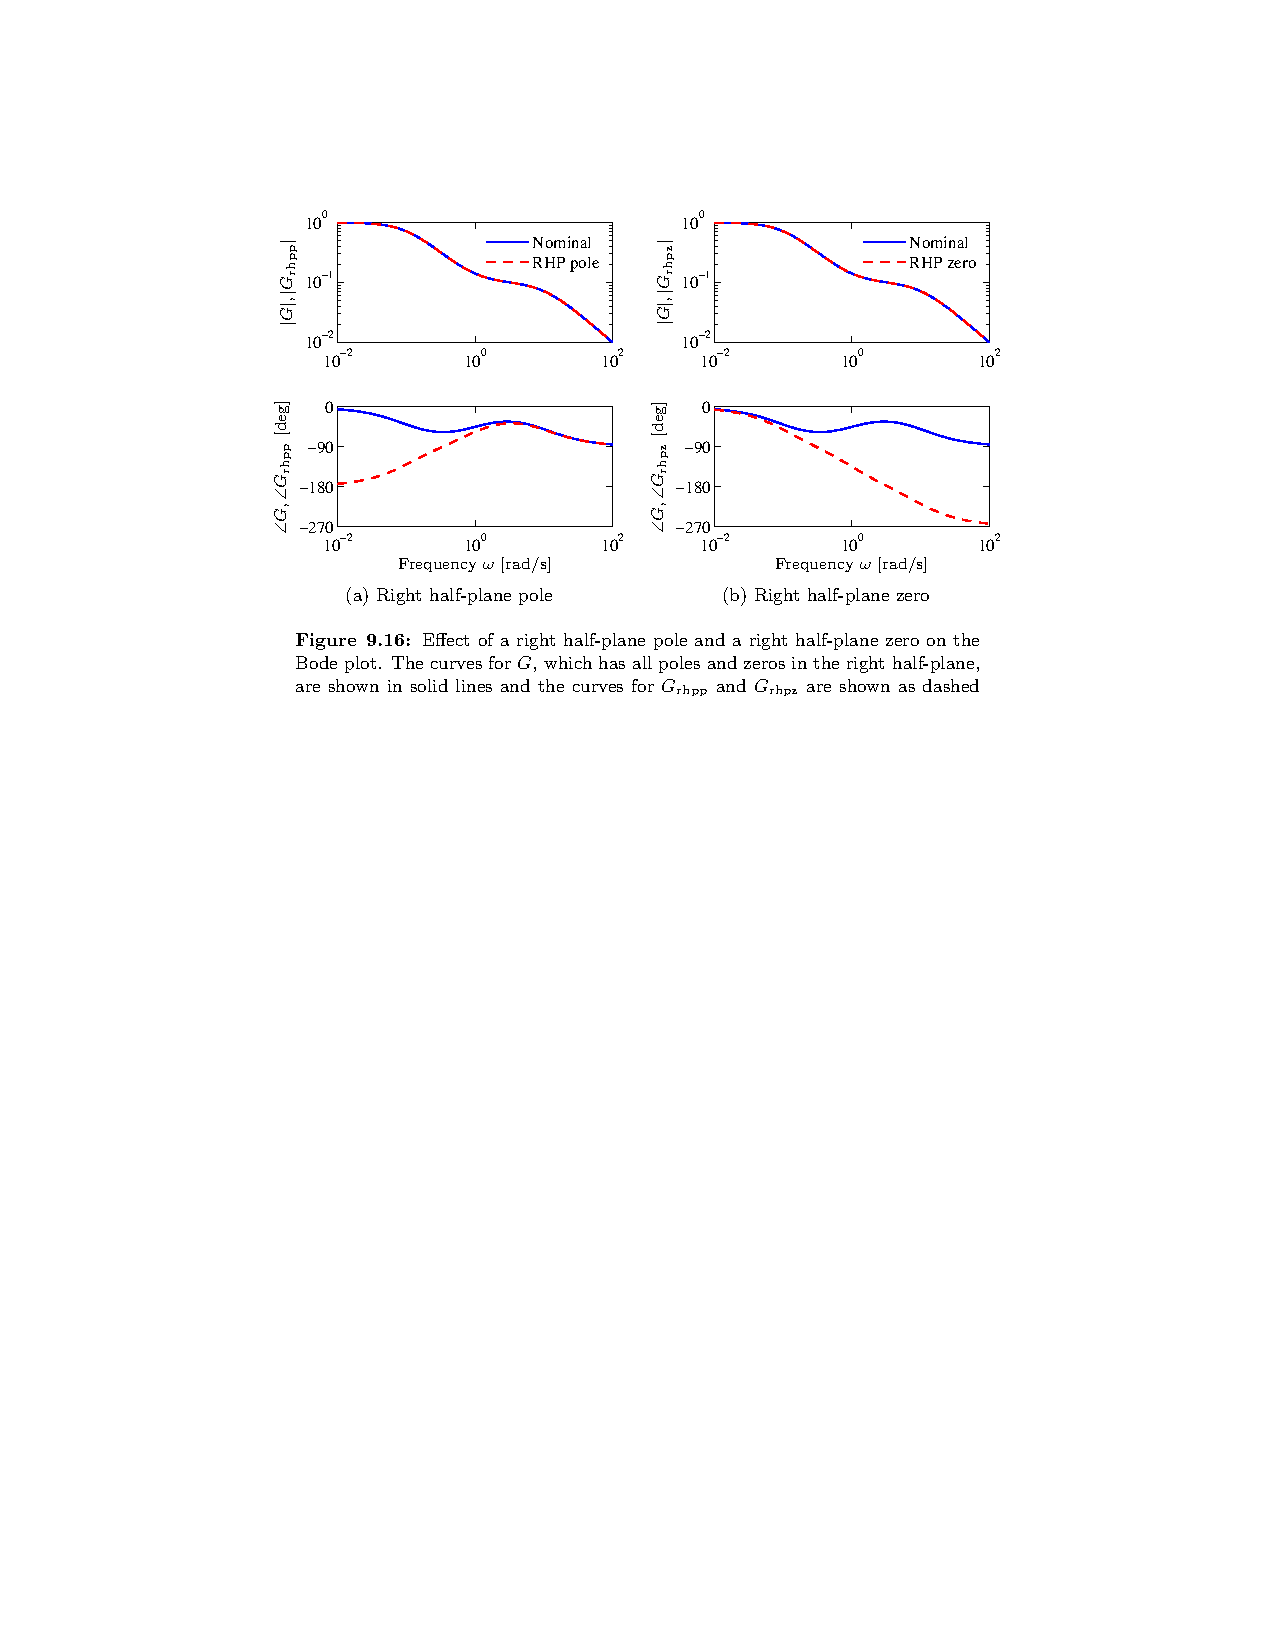
\includegraphics[width=0.8\linewidth]{figure9.16}

\end{frame}

\SUBCONCEPT{Time delays}

\begin{frame}
  \begin{itemize}
    \item  Time delays can cause stability problems
    \item  `Time delay' can mean:
    \begin{itemize}
      \item  Delays in reading data from a sensor
      \item  Delays in the control system
      \item  Delays in sending commands to the actuator
    \end{itemize}
    \item Can analyse problems from time delays but often can't overcome them with control
  \end{itemize}
\end{frame}

\begin{frame}{Pure delay}
\begin{columns}
\column{0.5\linewidth}
  \[
    G_{\mathrm{delay}} = \Exp{-\tau s}
  \]
\begin{itemize}
  \item No effect on magnitude
  \item $\theta_{\mathrm{delay}}=-\ww \tau$
  \item Reduces stability margins, leads to instability
\end{itemize}

\column{0.5\linewidth}
    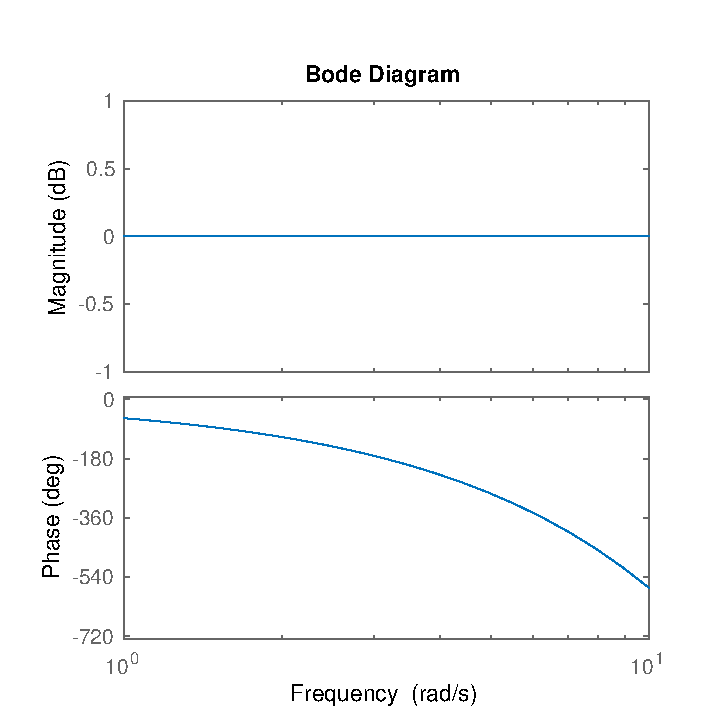
\includegraphics[width=\linewidth]{puretimedelaybode}
\end{columns}
\end{frame}

\begin{frame}
\frametitle{Padé approximation}
The exponential delay term $\exp(-s\tau)$ is not a rational function,
so we often approximate it using the \alert{Padé approximation}.

This begins with the Maclaurin series of the delay, but we can't use this directly because truncating the series doesn't give us a well-behaved transfer function:
\begin{align}
\Exp{-\tau s} &= 1 - \tau s + \frac{1}{2!}(\tau s)^2 - \dots + \frac{(-1)^n}{n!}(\tau s)^n + \dots 
\end{align}

The Padé approximation of order $n$ is a ratio of polynomials that matches the series up to the same order:
\begin{align}\label{eq:pade}
\Exp{-\tau s} &\approx \mathrm{PD}(\tau,n) = \frac{ \sum_{k=0}^n (-1)^k c_k (\tau s)^k  }
                            { \sum_{k=0}^n        c_k (\tau s)^k  } \,, &
          c_k &= \frac{ (2n-k)!n! }{ (2n)!k!(n-k)! }
\end{align}

\end{frame}

\begin{frame}
\frametitle{Just in case that equation is not self-evident}

What does `matching the series' mean? Consider for $\tau=2$:
\begin{align}
e^{-2s} = 1 - 2s + 2s^2 - \tfrac{4}{3}s^3 + \tfrac{2}{3}s^4 - \cdots
\end{align}
The Padé approximation for $n=1$ is:
\begin{align}\label{eq:pd21}
\mathrm{PD}(2,1) = \frac{1 - \frac{1}{2}(2s)}{1 + \frac{1}{2}(2s)} = \frac{1 - s}{1 + s}
\end{align}
The Taylor series expansion of \eqref{pd21} around $s=0$ is:
\begin{align}
\frac{1 - s}{1 + s} &= \bigl(1 - s\bigr)\bigl(1 - s + s^2 - s^3 + \cdots\bigr) \\
& = \underbrace{\strut 1 - 2s + 2s^2}  \underbrace{\strut -2s^3 + 2s^4 - \cdots}
\end{align}
\end{frame}

\begin{frame}
\frametitle{Padé examples}

Eq \eqref{pade} looks frightful but you can see the pattern:
\begin{align}
\mathrm{PD}(2,1) &= \frac{  -s + 1 }{  \phantom{+}s + 1 } 
\end{align}
\begin{align}
\mathrm{PD}(2,2) &= \frac{  s^2 - 3 s + 3 }{  s^2 + 3 s + 3 } 
\end{align}
\begin{align}
\mathrm{PD}(2,4) &= \frac{ -s^3 + 6 s^2 - 15 s + 15 }{  \phantom{+}s^3 + 6 s^2 + 15 s + 15 }
\end{align}
\end{frame}

\begin{frame}
\frametitle{Padé outputs ($n=\{1,3,5,7\}$)}

\centerline{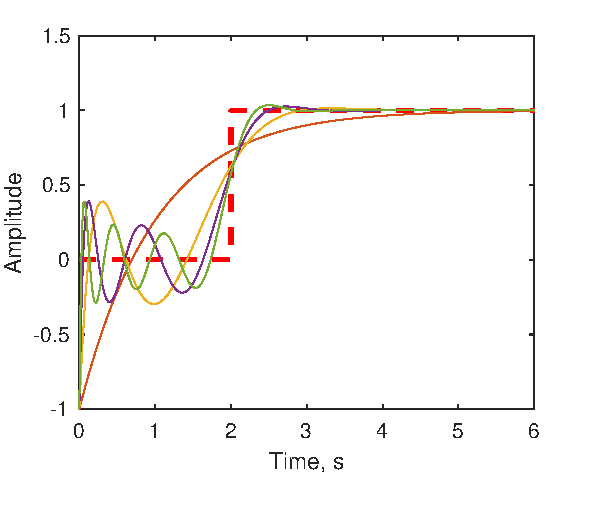
\includegraphics[width=0.5\linewidth]{pade-step.pdf}
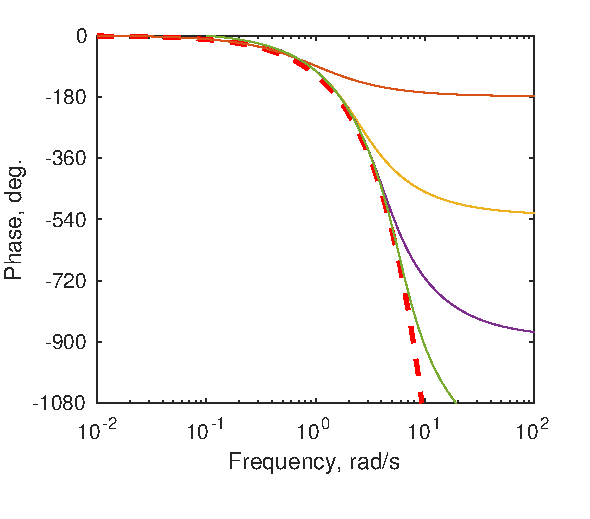
\includegraphics[width=0.5\linewidth]{pade-phase.pdf}}


\end{frame}

\SUBCONCEPT{System Insights from the Bode Plot}

\begin{frame}{Magnitude vs frequency, and phase vs frequency}
  \begin{itemize}
    \item  Used to analyse open loop \emph{and} closed loop
    \item  Frequency is explicit in the graph(s)
    \item  Changes in gain easily interpreted and visualised
    \begin{itemize}
      \item  When inverting just flip
    \end{itemize}
    \item  Time delays and phase lag also easily seen
    \item  Log / dB shows magnitude clearly over many orders of magnitude
\begin{itemize}
  \item Often express $a$ in dB with: $20\log_{10}(a)$
  \item $+\SI{20}{dB} \equiv \times 10$
  \item $-\SI{20}{dB} \equiv \times 0.1$
  \item $+\SI{6}{dB}  \equiv \times 2$
  \item $-\SI{3}{dB}  \equiv \times 1/\sqrt{2} \approx \times 0.707$
\end{itemize}
  \end{itemize}
\end{frame}

\begin{frame}{Resultant properties}
  Use Bode plots to discuss: (non-exhaustive list!)
  \begin{itemize}
    \item  DC gain
    \item  Bandwidth
    \item  Peak response and its frequency
    \item  Low frequency magnitude slope
    \item  High frequency magnitude slope (`roll-off')
    \item  Low frequency phase limit
    \item  High frequency phase limit
  \end{itemize}
\end{frame}


\begin{frame}{The Bode plot gives a quick overview of a system}
Frequency response perspective: the system is a filter which changes the amplitude and phase of an input signal

\vfill
\centering
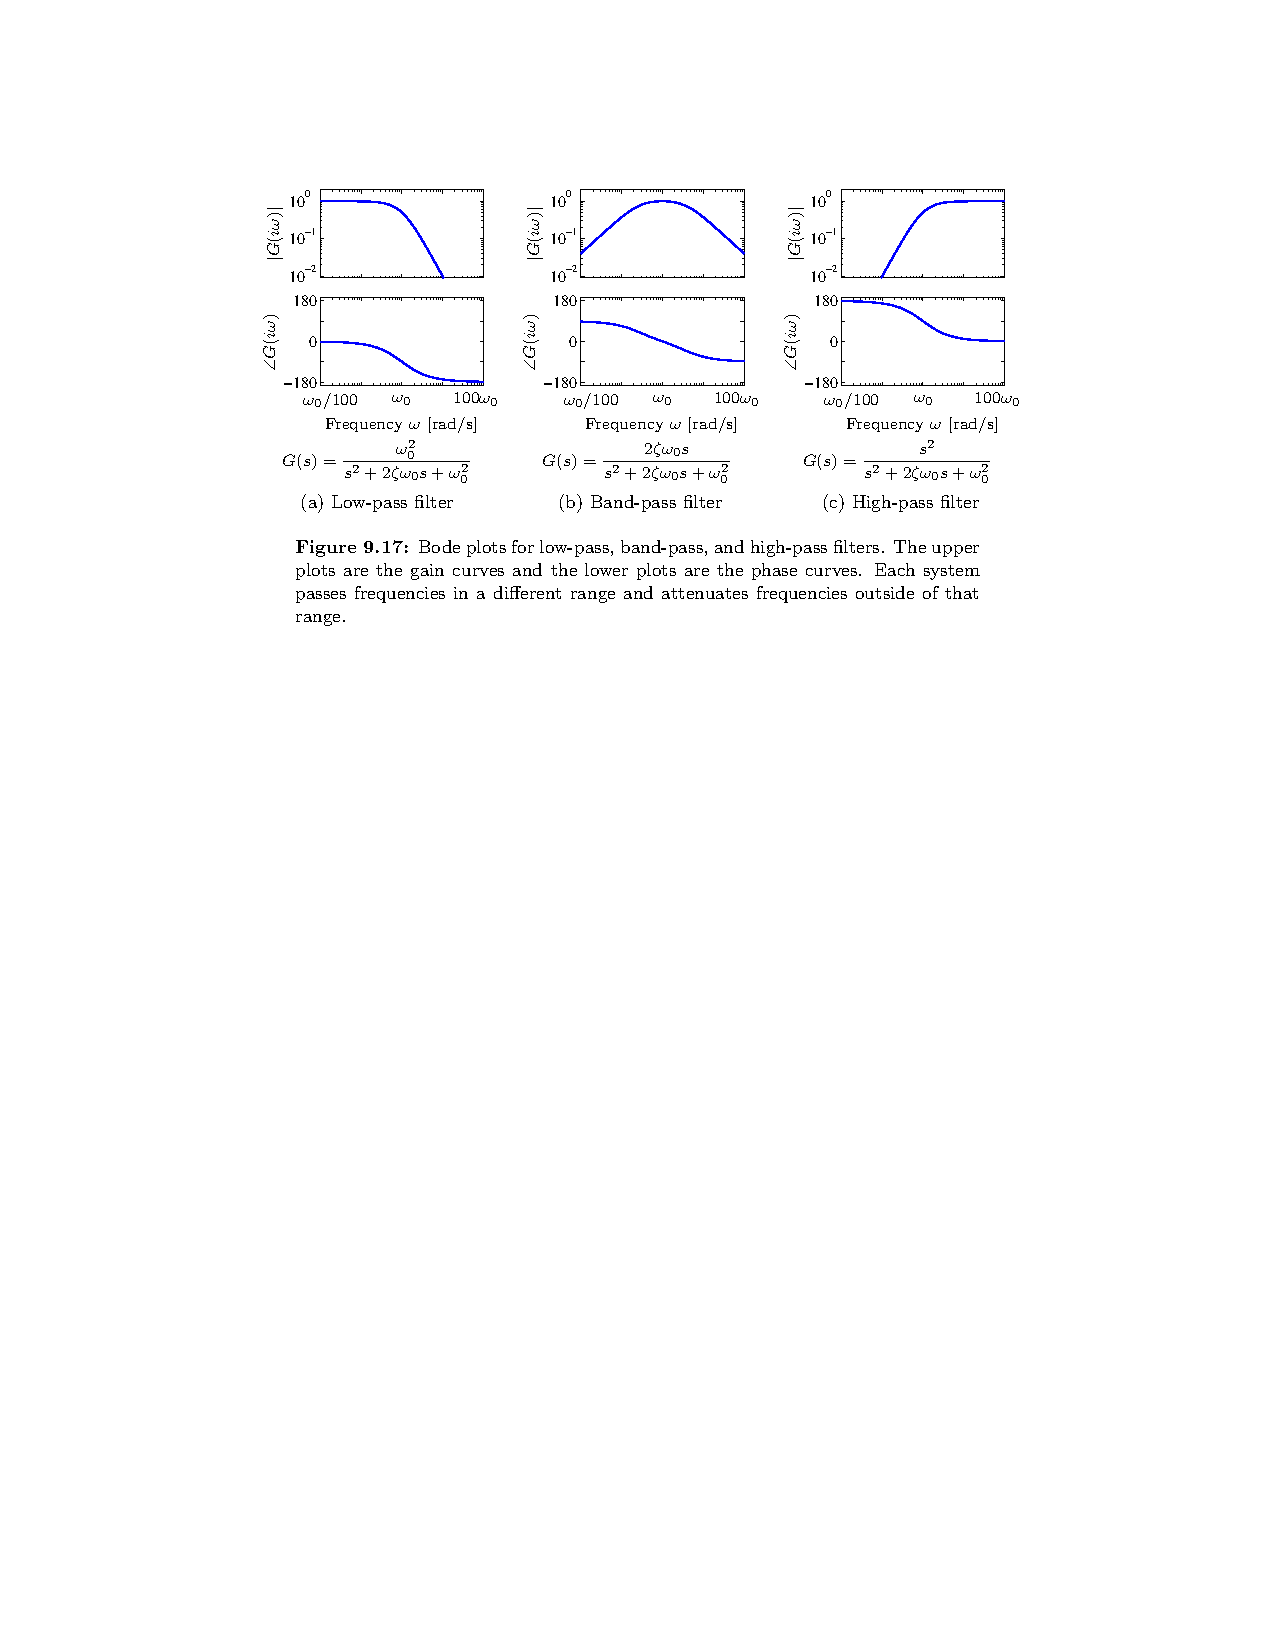
\includegraphics[width=0.8\linewidth]{figure9.17}

\end{frame}

\begin{frame}
\frametitle{Example 9.15 Spring--mass system}

\centering
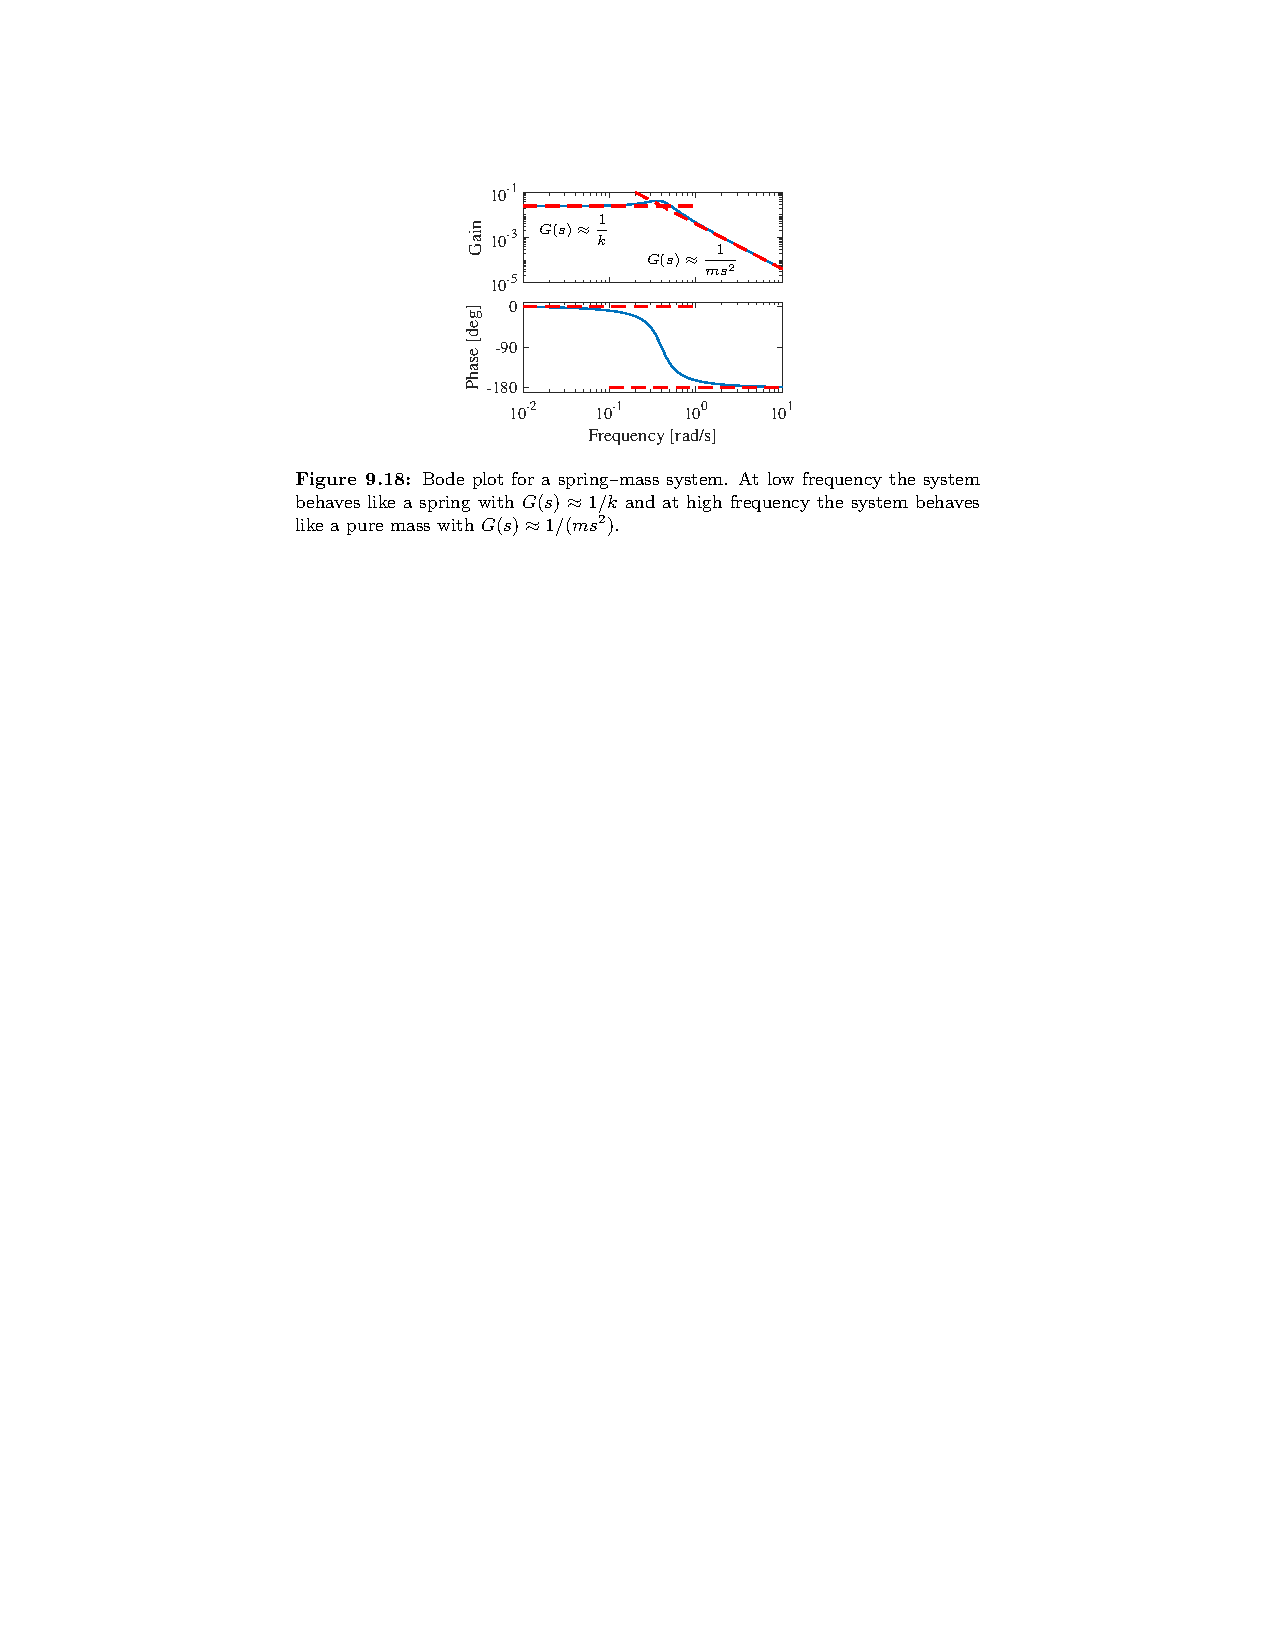
\includegraphics[width=\linewidth]{figure9.18}


\end{frame}


\SUBCONCEPT{Determining Transfer Functions Experimentally}

\begin{frame}{Measuring the FR}
Excite the system in one of three ways:
\begin{itemize}
\item iterate one frequency at a time
\item chirp (ascending or descending or both)
\item white noise
\end{itemize}
The second two methods require the FFT to calculate the FRF:
\begin{itemize}
\item Chirp: FFT size is length of chirp, no windowing
\item Random noise: FFT size as desired, usually use Hanning window
\end{itemize}
Usually avoid using Matlab's \texttt{fft} command --- use \texttt{pwelch} and \texttt{tfestimate} instead.
\end{frame}

\begin{frame}
\frametitle{System identification}
\centering

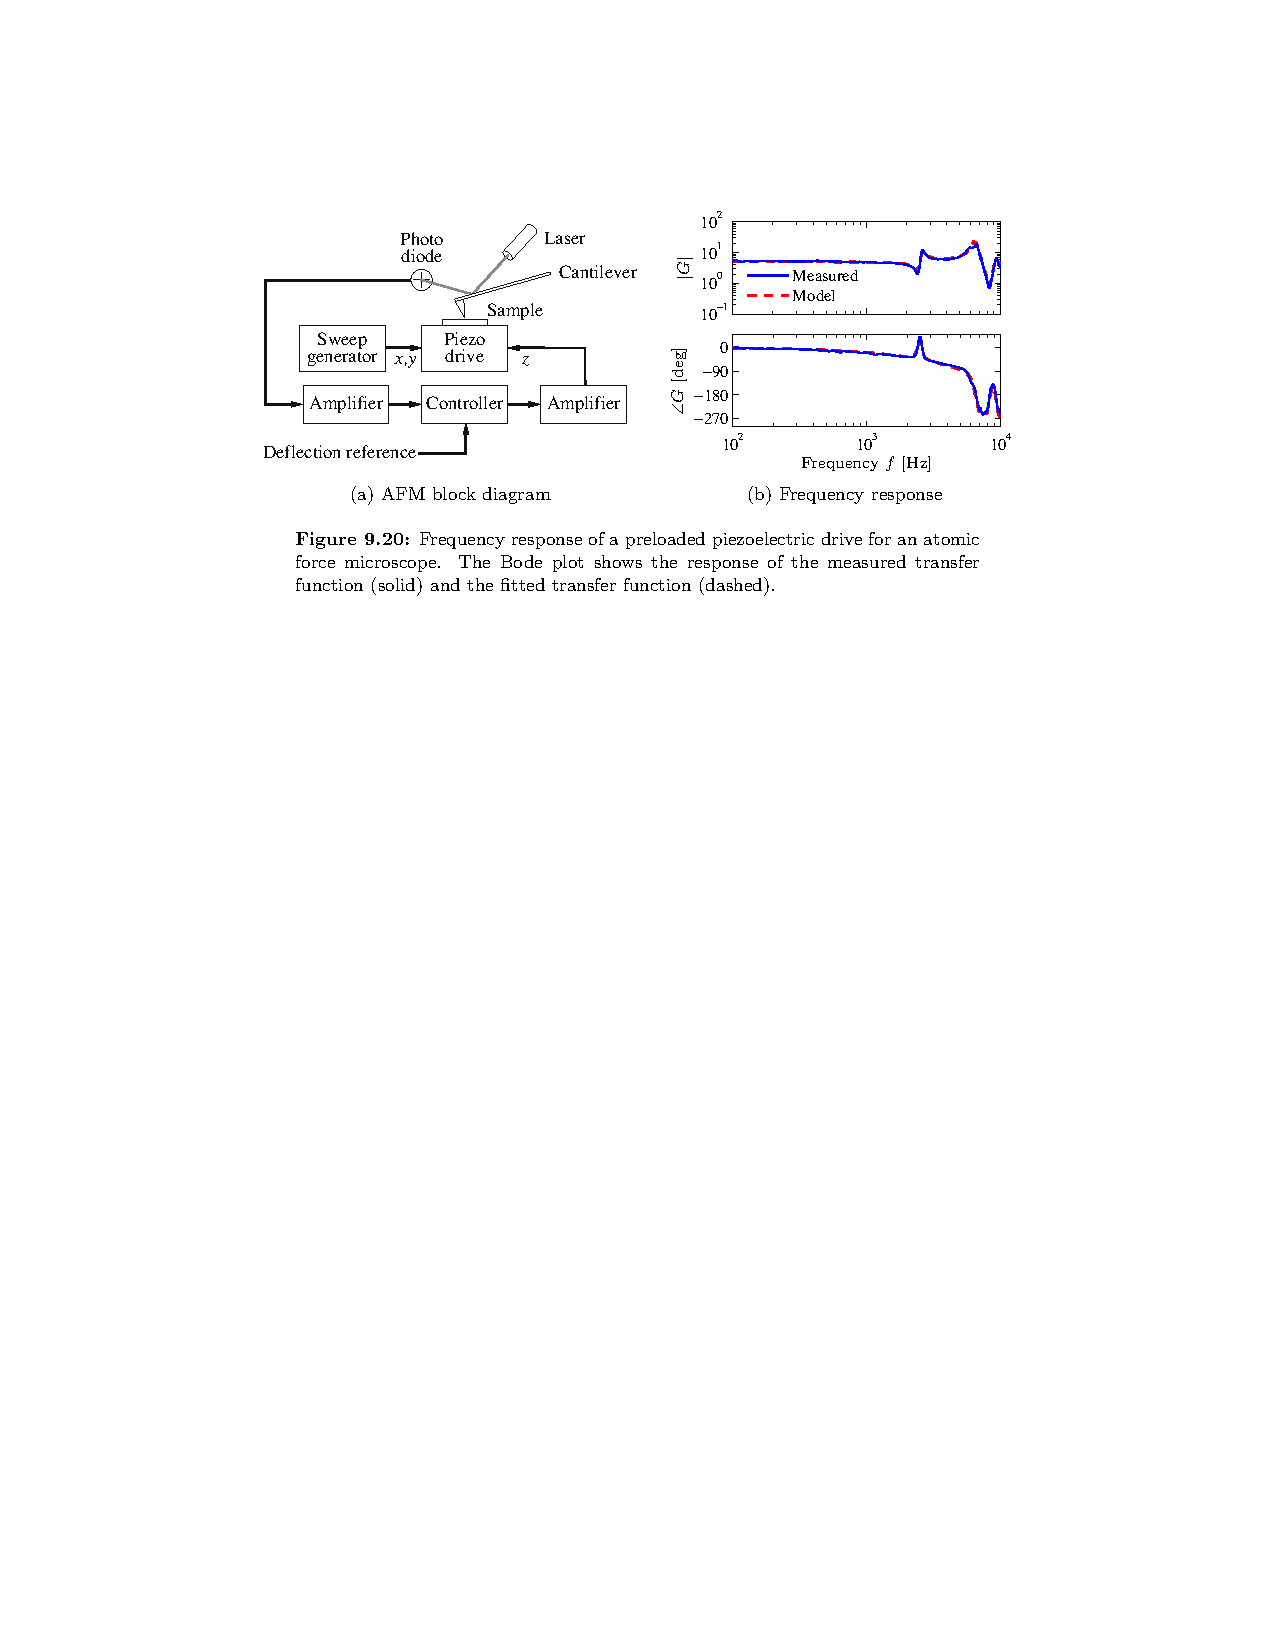
\includegraphics[width=0.7\linewidth]{figure9.20}

\hrulefill
\vfill

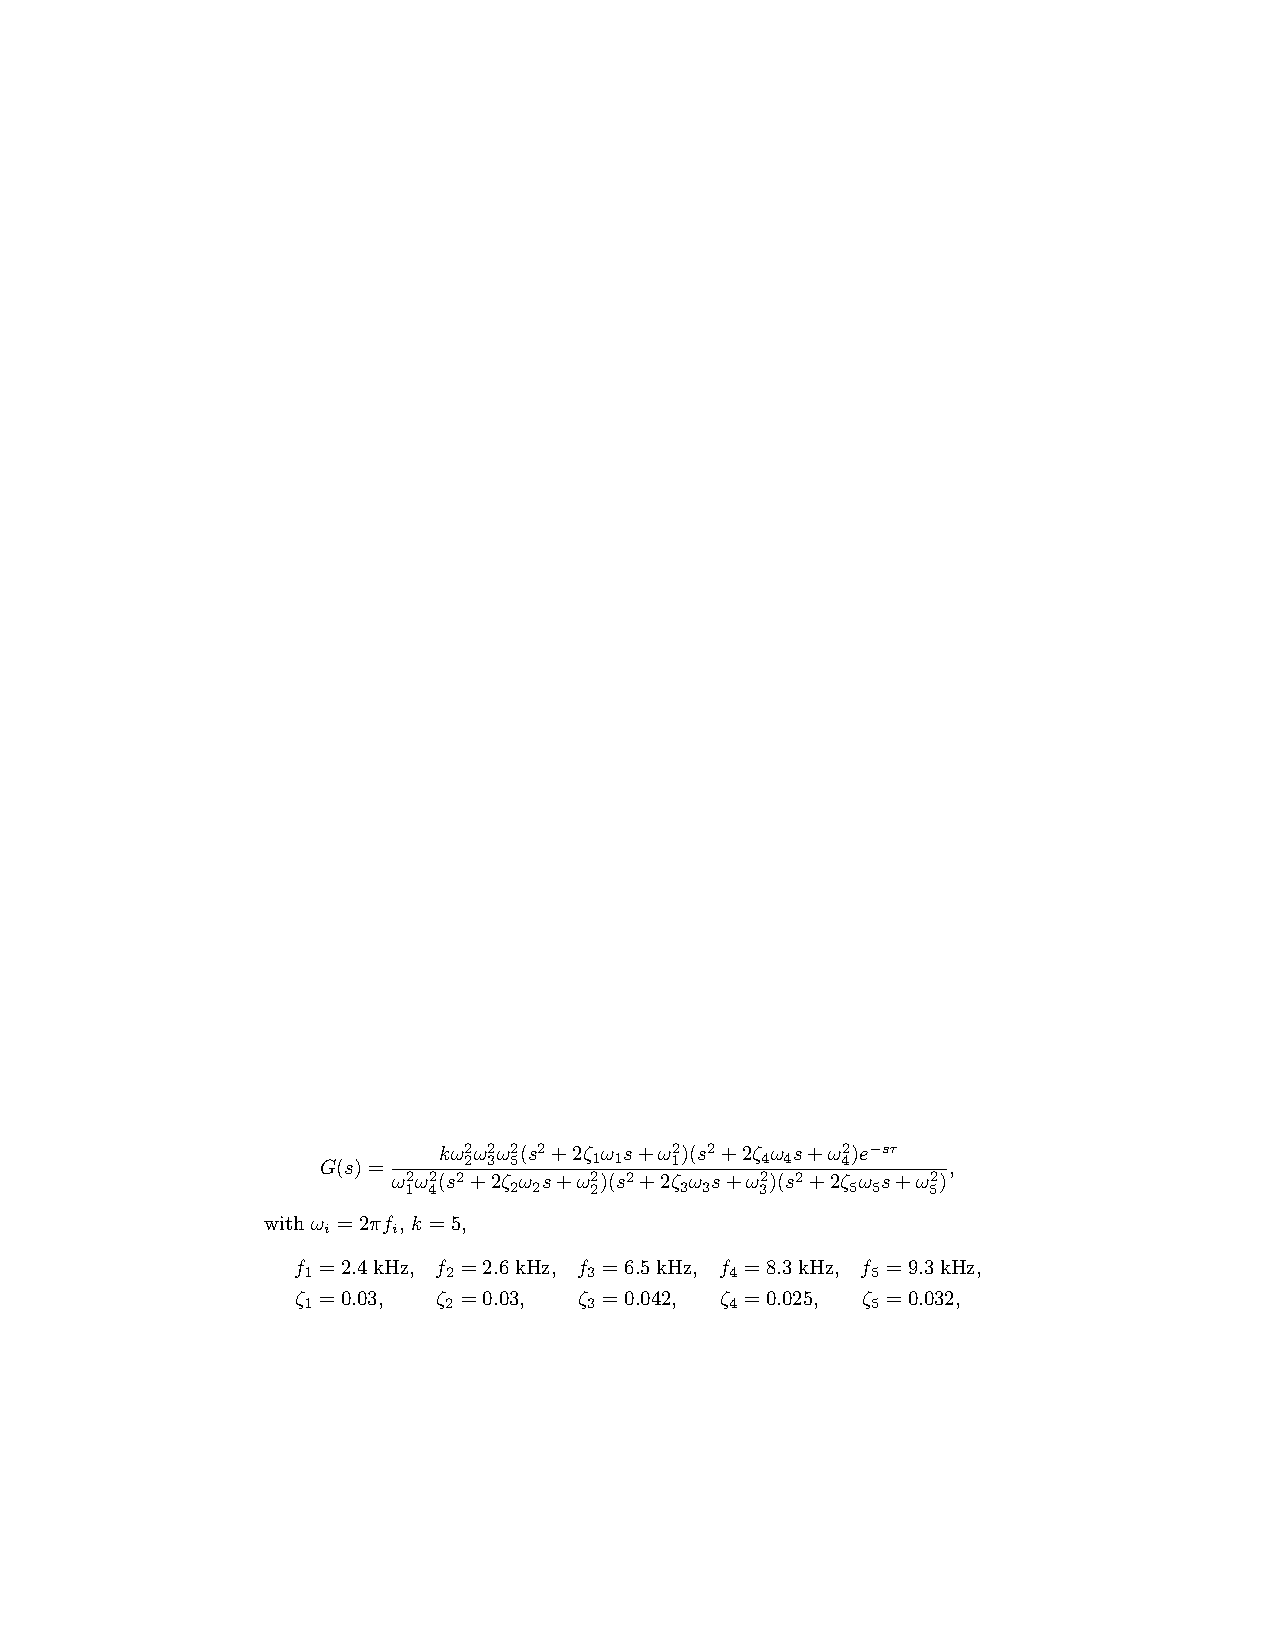
\includegraphics[width=0.7\linewidth]{example9.17}


\end{frame}

\begin{frame}
\frametitle{Matlab example --- sysid from time-domain data}

\small
\begin{columns}
\column{0.5\textwidth}
From System Identification Toolbox: (example in \texttt{doc tfest})
\includematlab{tfest_test.m}{load}

\column{0.5\textwidth}
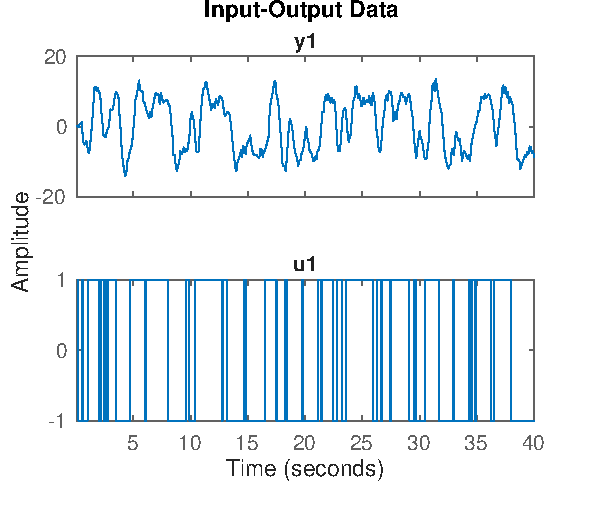
\includegraphics[width=\linewidth]{idtime}

\end{columns}

\end{frame}

\begin{frame}
\frametitle{Matlab example --- sysid from time-domain data}
\small

\begin{columns}
\column{0.5\textwidth}
\includematlab{tfest_test.m}{frf}

\column{0.5\textwidth}
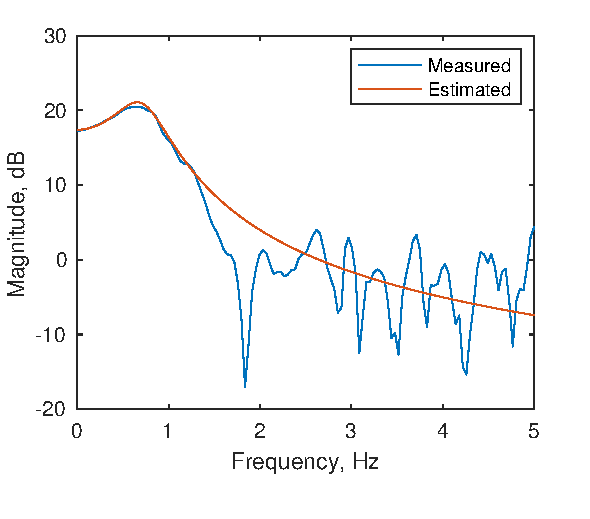
\includegraphics[width=\linewidth]{idfreq}
\end{columns}
\end{frame}

\SUMMARYFRAME
\FINALE

\end{document}





\TOPIC{Frequency Domain Analysis}

  \documentclass{beamer-control}
\usepackage{beamer-control-singlefile}
\INCLUDEONLY{The Loop Transfer Function}
\begin{document}
\CONCEPT{The Loop Transfer Function}

\begin{SUMMARY}
\begin{itemize}
\item Loop analysis
\item Calculating the loop transfer function
\end{itemize}
\vfill References:
\begin{itemize}
\item \astrom{§10.1}
\end{itemize}
\end{SUMMARY}



\SUBCONCEPT{Loop analysis}

\begin{frame}{Frequency in feedback}
\begin{itemize}
\item How may we assess the behaviour of a closed loop system by studying the open loop system properties?
\item Using transfer functions we can follow how a sinusoidal signal at a given frequency behaves in the feedback loop
\item We can then assess stability of the closed loop by noticing if this signal grows or decays - if it grows, we have an unstable system
\end{itemize}
\end{frame}

\begin{frame}{Loop transfer function}
Rather than calculating the characteristic polynomial of the closed loop system (which is limited in aiding design of a controller), we may instead analyse the \textit{loop transfer function}
\[L(s)=P(s)C(s)\]
which represents the transfer function from input at A to output at B multiplied by $-1$ (to account for negative feedback).

\begin{figure}
	\centering
	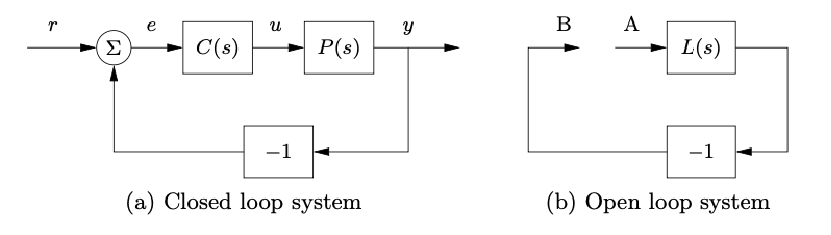
\includegraphics[width=\linewidth]{figure10.1}
	\\
	\textbf{Figure 10.1:} The loop transfer function.
\end{figure}
\end{frame}

\begin{frame}{Condition for stability}
	
\begin{itemize}
	\item Consider inputting a sinusoidal input of frequnecy $\omega_0$ at A
	\item To maintain the oscillation, the signal at B will also be a sinusoid with frequency $\omega_0$ and therefore
	\[L(i\omega_0)=-1.\]
	\item This condition says that our frequency response passes through the value of $-1$, known as the \textit{critical point}
	\item If we require stability at a freuqency $\omega_c$ such that $\angle L\left(i \omega_{\mathrm{c}}\right)=180^{\circ}$, we therefore want our signal at B to have a smaller amplitude than the input at A and so $|L(i\omega_c)|<1$
\end{itemize}
\end{frame}


\SUBCONCEPT{Calculating the loop transfer function}

\begin{frame}{Example}
\begin{itemize}
\item Consider an electric motor with inertia $J$ and damping $c$ with proportional feedback controller and small delay in measurement of the motor position
\item The process dynamics are 
\[P(s) = \frac{k_I}{Js^2+cs}\]
\item The controller is of the form
\[C(s) = k_p\]
\item Therefore the loop transfer function (with added delay $\tau$) is 
\[L(s) = P(s) C(s) e^{-\tau s} = \frac{k_Ik_p}{Js^2+cs}e^{-\tau s}\]
\end{itemize}
\end{frame}

\begin{frame}{Example continued}
\begin{itemize}
\item The magnitude of the transfer function does not change with the delay but the phase does
\item Therefore we may get oscillations in the closed loop system if delay is present
\item We can use the Bode plots of the loop transfer function to assess what the magnitude of the output signal of the loop transfer function is correspondoing to a phase of $180^\circ$
\item If $\theta_0$ is the phase of the undelayed system at a frequency $\omega_0$, then a time delay of 
\[\tau_c=\frac{\pi+\theta_0}{\omega_0}\]
will cause $L(i\omega_0)$ to be equal to $-1$
\end{itemize}
\end{frame}


\begin{frame}{Example continued}
\begin{itemize}
\item For no delay $\tau=0$, the phase of $L(s)$ approaches $180^\circ$ but doesn't reach it and so the system is stable
\item For a delay of $\tau=\tau_c$, when the phase of $L(s)$ is $180^\circ$, the magnitude is $1$ and so the system maintains oscillation
\item For a delay of $\tau=3\tau_c$, the corresponding magnitude at $180^\circ$ phase is greater than $1$, resulting in instability
\end{itemize}
\begin{figure}
\centering
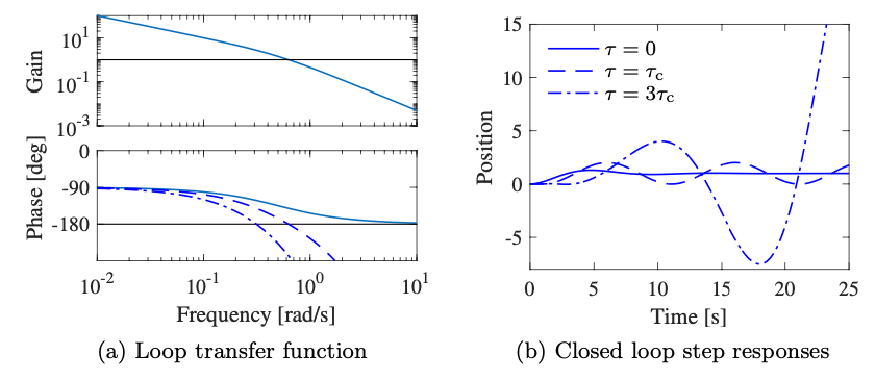
\includegraphics[width=0.8\linewidth]{figure10.3}
\\
\textbf{Figure 10.3:} The loop transfer function and step response for electric motor control system.
\end{figure}

\end{frame}


\SUMMARYFRAME
\FINALE

\end{document}

  \documentclass{beamer-control}
\usepackage{beamer-control-singlefile}
\INCLUDEONLY{The Nyquist Criterion}
\begin{document}
\CONCEPT{The Nyquist Criterion}

\begin{SUMMARY}
\begin{itemize}
\item Nyquist plot
\item Nyquist criterion
\end{itemize}
\vfill References:
\begin{itemize}
\item \astrom{§10.2}
\end{itemize}
\end{SUMMARY}



\SUBCONCEPT{Nyquist plot}

\begin{frame}{Frequency response graphically}
\begin{itemize}
\item The dynamics of a linear system may be represented by its frequency response and graphically illustrated by a Bode plot
\item We may also graphically represent the frequency response on one graph by using a Nyquist plot, plotted on the complex plane
\item The Nyquist plot of a loop transfer function $L(s)$ is formed by tracing $s\in\mathbb{C}$ around the Nyquist contour $\Gamma$ (given by the imaginary axis combined with an arc at infinity connecting the endpoints of the imaginary axis)
\item At any point on the Nyquist plot corresponding to a frequency $s=\ii\omega$, the distance away from the origin gives the magnitude of the loop transfer function $L(s)$ and the angle with the imaginary axis gives the phase
\end{itemize}
\end{frame}


\begin{frame}{Nyquist plot}
\begin{figure}
	\centering
	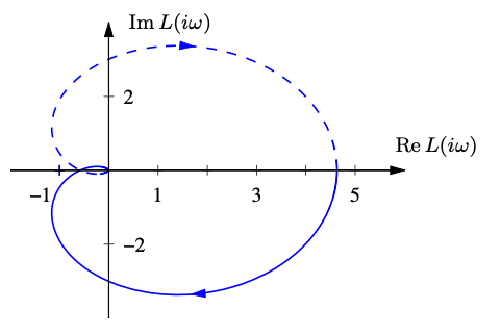
\includegraphics[width=0.9\linewidth]{figure10.5}
	\\
	\textbf{Figure 10.5:} Nyquist plot for $L(s) = {1}/{(s+0.6)^3}$.
\end{figure}
\end{frame}


\SUBCONCEPT{Nyquist criterion}

\begin{frame}{Condition for stability - Nyquist criterion}
\begin{itemize}
\item Let $L(s)$ be the loop transfer function for a negative feedback system and assume that $L$ has no poles in the closed right half-plane expect possible at the origin
\item Then the closed loop system 
\begin{align}
G_{cl}=\frac{L(s)}{1+L(s)}
\end{align}
is stable if and only if the image of $L$ along the closed contour $\Gamma$ has no net encirclements of the critical point $s=-1$
\item The number of encirclements is called the winding number
\item This criterion tells us how the stability of a system is influenced by changing the controller parameters
\end{itemize}
\end{frame}


\begin{frame}{Example}
\begin{itemize}
	\item Consider the transfer function 
	\[L(s) = \frac{k}{s(s+1)^2}\] 
	representing a third-order system with a pole at the origin with nominal gain value $k=1$
	\item The system has a single pole at $s=0$ and a double pole at $s=-1$
	\item The Bode plot thus has the slope $-1$ for low frequencies, and at the double pole the slope changes to $-3$
	\item The phase curve starts at $-90^\circ$ for low frequencies, is \ang{-180} at $\omega=1$ and is \ang{-270} at high frequencies
\end{itemize}
\end{frame}


\begin{frame}{Example continued}
	\begin{itemize}
		\item The Nyquist curve intersects the negative real axis at $\omega=1$ with $L(\ii)=-0.5$ for $k=1$
		\item The Nyquist curve only encircles the critical point $s=-1$ when the gain is $k\geq 2$ as $L(\ii)=-\tfrac{k}{2}$
	\end{itemize}
\begin{figure}
	\centering
	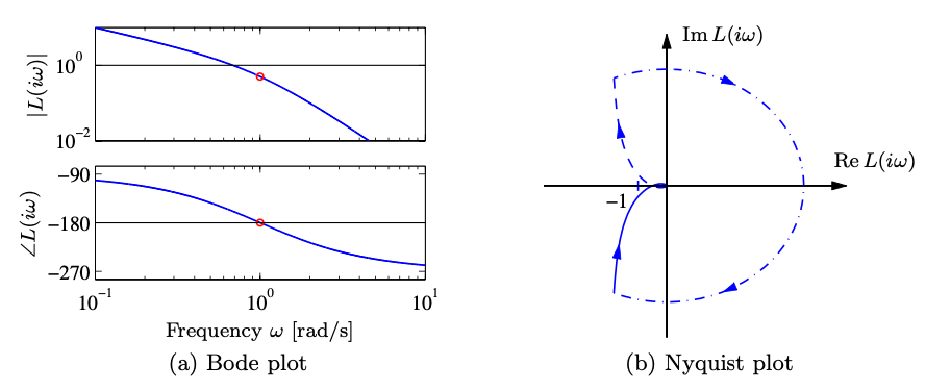
\includegraphics[width=0.9\linewidth]{figure10.6}
	\\
	\textbf{Figure 10.6:} Sketching Nyquist and Bode plots.
\end{figure}
\end{frame}

\SUMMARYFRAME
\FINALE

\end{document}

  \documentclass{beamer-control}
\usepackage{beamer-control-singlefile}
\INCLUDEONLY{Stability Margins}
\begin{document}
\CONCEPT{Stability Margins}

\begin{SUMMARY}
\begin{itemize}
\item Descriptions of stability
\item Calculating stability margins
\end{itemize}
\vfill References:
\begin{itemize}
\item \astrom{§10.3}
\end{itemize}
\end{SUMMARY}



\SUBCONCEPT{Descriptions of stability}

\begin{frame}{How stable is a system?}
\begin{itemize}
\item The Nyquist criterion tells us when a system will be unstable in closed loop -- dependent on encirclement of the critical point
\item In practice, a system may be stable but very close to instability and so we would like a way to capture how far from instability a system is
\item Stability margins express how well the Nyquist curve of a system avoids the critical point by representing how much gain or phase must be added to the system to make it unstable
\item This tells us how robust the system is to perturbation or control parameters
\end{itemize}
\end{frame}



\begin{frame}{Different margins}
There are three types of margin to assess stability
\begin{itemize}
	\item The stability margin $s_m$ describes the shortest distance of the Nyquist curve to the critical point
	\item As increasing the controller gain expands the Nyquist curve radially, the gain margin $g_m$ is defined as the smallest multiplier of the loop gain that makes the system unstable (recommended range $2<g_m<5$)
	\item As increasing the phase of the controller turns the Nyquist curve clockwise, the phase margin $\varphi_m$ is the amount of phase lag required to make the system unstable (recommended range $30^\circ < \varphi_m < 60^\circ$)
\end{itemize}
The gain and phase margins may also be determined from the Bode plots
	
\end{frame}

\SUBCONCEPT{Calculating stability margins}

\begin{frame}{Margins from Nyquist}
\begin{itemize}
	\item The stability margin $s_m$ is determined by finding the closest point on the Nyquist curve to the critical point and calculating this distance
	\item The gain margin $g_m$ is the inverse of the distance between the origin and the point between $-1$ and $0$ where the loop transfer function crosses the negative real axis
	\item The phase margin $\varphi_m$ is the angle between the the negative real axis and the line joining the origin with the point where the loop transfer function intersects the unit circle below the real axis
\end{itemize}
\end{frame}

\begin{frame}{Margins from Nyquist}
\begin{figure}
	\centering
	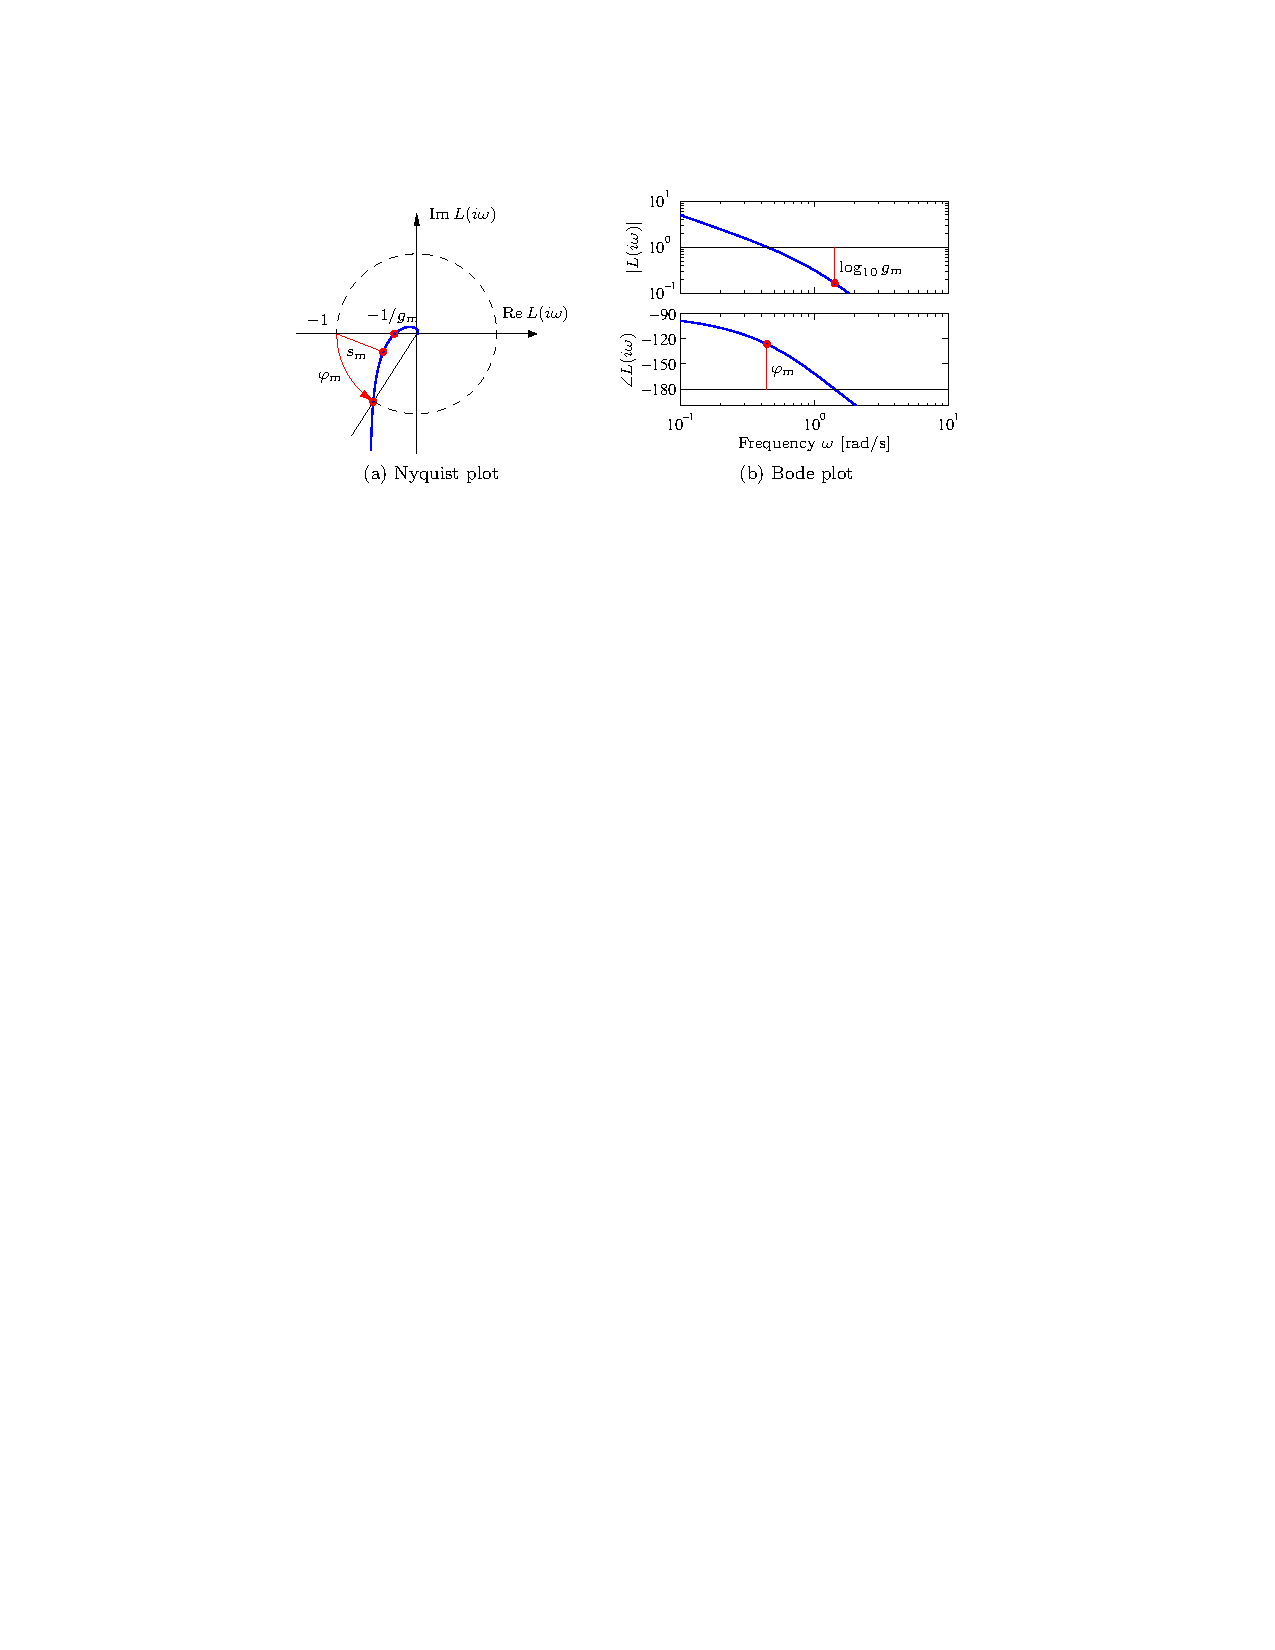
\includegraphics[width=0.9\linewidth]{figure10.11}
	\\
	\textbf{Figure 10.11:} Stability margins for a third-order loop transfer function.
\end{figure}
\end{frame}


\begin{frame}{Example}
\begin{itemize}
	\item Consider the loop transfer function $L=\tfrac{3}{(s+1)^3}$
	\item From the Nyquist plot we get $s_m=0.464$, $g_m = 2.67$, $\varphi=41.7^\circ$
\end{itemize}
\begin{figure}
	\centering
	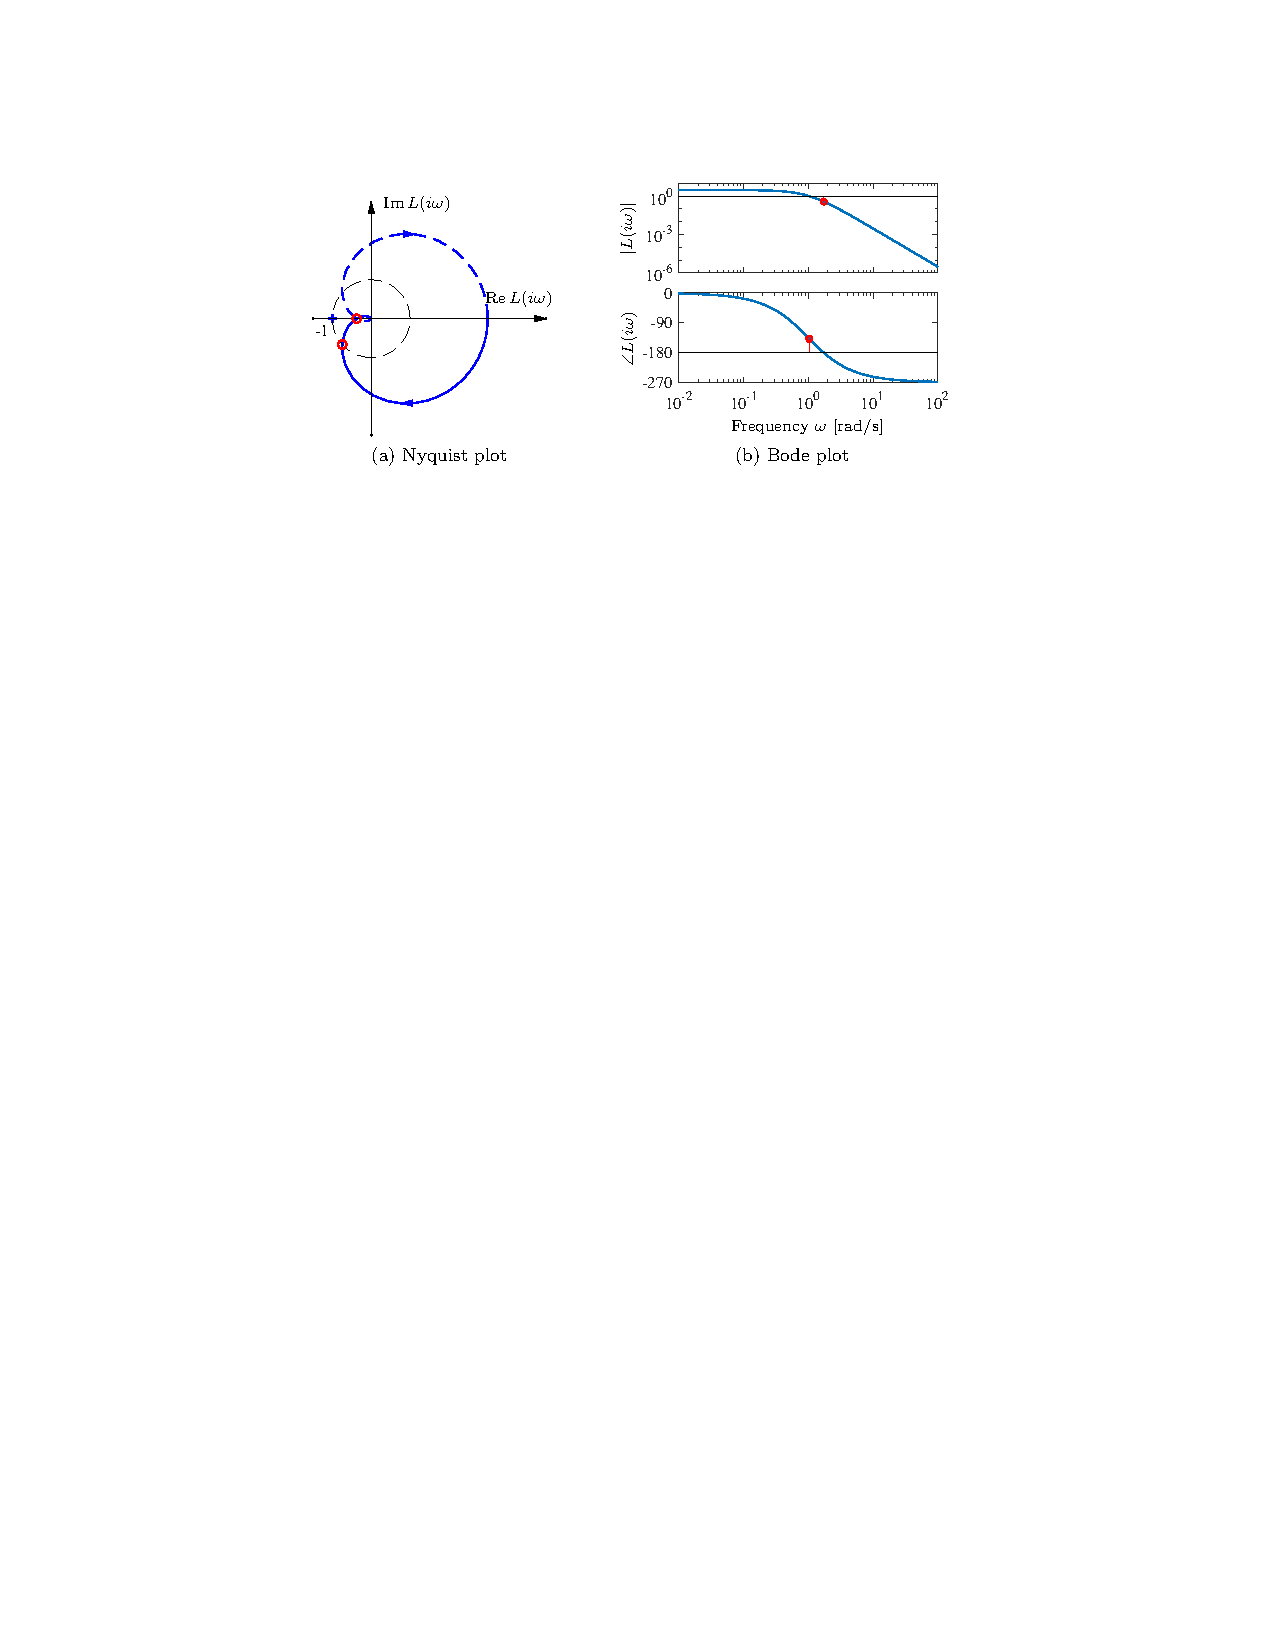
\includegraphics[width=0.9\linewidth]{figure10.12}
	\\
	\textbf{Figure 10.12:} Stability margins for a third-order loop transfer function.
\end{figure}
\end{frame}

\SUMMARYFRAME
\FINALE

\end{document}

  \documentclass{beamer-control}
\usepackage{beamer-control-singlefile}
\INCLUDEONLY{Bode’s Relations and Minimum Phase Systems}
\begin{document}
\CONCEPT{Bode’s Relations and Minimum Phase Systems}

\begin{SUMMARY}
\begin{itemize}
\item Yyy
\end{itemize}
\vfill References:
\begin{itemize}
\item \astrom{Chapter Z}
\end{itemize}
\end{SUMMARY}



\SUBCONCEPT{This is a Subconcept}

\begin{frame}{This is a slide}
\begin{itemize}
\item a
\item b
\end{itemize}
\end{frame}


\SUBCONCEPT{This is another Subconcept}

\begin{frame}{This is another slide}
\begin{itemize}
\item c
\item d
\end{itemize}
\end{frame}


\SUMMARYFRAME
\FINALE

\end{document}



\MODULE{Control System Design}

\TOPIC{PID Control}

  \documentclass{beamer-control}
\usepackage{beamer-control-singlefile}
\INCLUDEONLY{Basic Control Functions}
\begin{document}
\CONCEPT{Basic Control Functions}

\begin{SUMMARY}
\begin{itemize}
\item PID controller structure
\item P, I and D
\end{itemize}
\vfill References:
\begin{itemize}
\item \astrom{§11.1}
\end{itemize}
\end{SUMMARY}



\SUBCONCEPT{PID controller structure}

\begin{frame}{Control without a model}
\begin{itemize}
\item The PID controller is composed of three terms -- the proportional term (P) which depends on the present error, the integral term (I) which depends on the past error, and the derivative term (D) which depends on the future errors
\item Rather using a full state feedback controller based on a prediction of the future state of a system using a mathematical model, the PID controller uses linear extrapolation of the measured output for control
\item PID controllers are ubiquitous in industrial applications due to their wide applicability, ease of implementation, and avoidance of using a model
\end{itemize}
\end{frame}

\begin{frame}
\begin{figure}
	\centering
	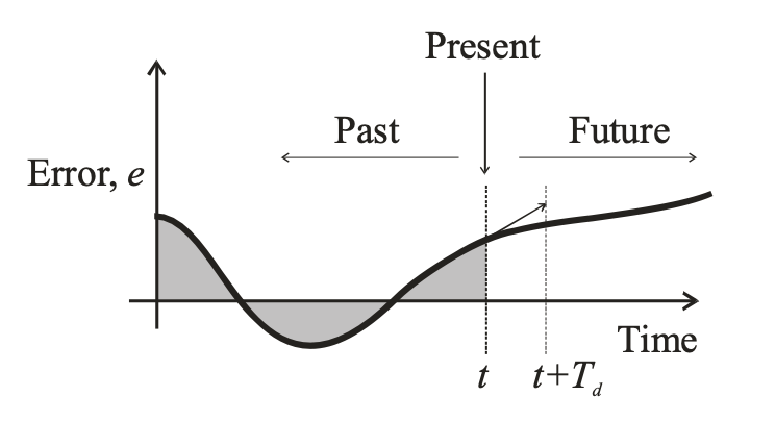
\includegraphics[width=0.8\linewidth]{figurePID1}
	\\
	\textbf{Figure:} Diagram describing the role of the three PID terms. 
\end{figure}
\end{frame}

\begin{frame}{Control action}
\begin{itemize}
	\item The control action of a PID controller is dependent on proportional feedback, integral action, and derivative action
	\[u=k_{p} e+k_{i} \int_0^t e(\tau) \, \mathrm{d} \tau+k_{d} \frac{\mathrm{d} e}{\mathrm{d} t}\]
	where $k_p$ is the proportional gain, $k_i$ is the integral gain, and $k_d$ is the derivative gain
	\item The integral time constant $T_i=\tfrac{k_p}{k_i}$ and derivative time constant $T_d = \tfrac{k_d}{k_p}$ provide an alternate parameterisation for the control action
	\[u = k_{p}\left(e+\frac{1}{T_{i}} \int_0^t e(\tau) \, \mathrm{d} \tau+T_{d} \frac{\mathrm{d} e}{\mathrm{d} t}\right)\]
\end{itemize}

\end{frame}


\begin{frame}
\begin{figure}
	\centering
	\includegraphics[width=0.8\linewidth]{figure11.1}
	\\
	\textbf{Figure 11.1:} Block diagram of PID controller in closed loop system. 
\end{figure}
\end{frame}

\SUBCONCEPT{P, I and D}

\begin{frame}{Effects of the three terms}
\textbf{Proportional feedback}
\begin{itemize}
\item With only proportional feedback, non-zero steady-state error is common
\item Increasing the proportional gain $k_p$ will reduce the error but make the system more oscillatory
\item Too high of a gain may make the system unstable 
\item Proportional band also used, $PB=\tfrac{100}{k_p}$
\end{itemize}
\textbf{Integral feedback}
\begin{itemize}
	\item We saw in the Topic 4 - State Feedback that integral action guarantees that if a steady state exists, we will reach it with integral control
	\item An increase in the integral gain $k_i$ makes the system robust to disturbances
	\item Too high of a gain results in oscillatory behaviour, poor robustness, and possible instability
\end{itemize}
\end{frame}


\begin{frame}{Effects of the three terms}
	\textbf{Derivative feedback}
	\begin{itemize}
		\item Derivative control provides predictive or anticipatory action
		\item An increase in the derivative gain $k_d$ adds damping into the system
		\item Reduces overshoot
	\end{itemize}
\end{frame}

\begin{frame}{PID control in action}
\begin{figure}
	\centering
	\includegraphics[width=\linewidth]{figure11.2}
	\\
	\textbf{Figure 11.2:} Responses to step changes in the reference value for a system with a proportional controller (a), PI controller (b), and PID controller (c).. 
\end{figure}
\end{frame}


\SUMMARYFRAME
\FINALE

\end{document}

  \documentclass{beamer-control}
\usepackage{beamer-control-singlefile}
\INCLUDEONLY{Simple Controllers for Complex Systems}
\begin{document}
\CONCEPT{Simple Controllers for Complex Systems}

\begin{SUMMARY}
\begin{itemize}
\item Yyy
\end{itemize}
\vfill References:
\begin{itemize}
\item \astrom{Chapter Z}
\end{itemize}
\end{SUMMARY}



\SUBCONCEPT{This is a Subconcept}

\begin{frame}{This is a slide}
\begin{itemize}
\item a
\item b
\end{itemize}
\end{frame}


\SUBCONCEPT{This is another Subconcept}

\begin{frame}{This is another slide}
\begin{itemize}
\item c
\item d
\end{itemize}
\end{frame}


\SUMMARYFRAME
\FINALE

\end{document}

  \documentclass{beamer-control}
\usepackage{beamer-control-singlefile}
\INCLUDEONLY{PID Tuning}
\begin{document}
\CONCEPT{PID Tuning}

\begin{SUMMARY}
\begin{itemize}
\item Tuning laws
\item Automatic tuning
\end{itemize}
\vfill References:
\begin{itemize}
\item \astrom{§11.3}
\end{itemize}
\end{SUMMARY}



\SUBCONCEPT{Tuning laws}

\begin{frame}{Achieving desired response}
	\begin{itemize}
		\item Designers and users of control systems frequently need to adjust parameters to achieve some desired behaviour
		\item There are many, many ways to do this and one conventional framework is to model the system and then follow the design process outlined previously
		\item For complicated, high-dimensional, nonlinear systems this can often be a tedious process
		\item The PID controller has very few parameters and due to its simplicity may be preferrable in these challenging settings
		\item Empirical tuning laws based on real systems have been developed for the adjustment of control parameters
	\end{itemize}
\end{frame}

\begin{frame}{Ziegler-Nichols' tuning}
\begin{itemize}
\item Ziegler and Nichols designed the first tuning laws in the 1940s
\item The idea is to perform an experiment on the process dynamics, extract information about the system in the time and frequency domains, and infer good choices for the PID gains
\end{itemize}
\end{frame}


\begin{frame}{Ziegler-Nichols' tuning - Time-domain method}
\begin{itemize}
	\item In the time domain method, the step response of a system is measured by inputting a unit step and measuring the output (or scaling the output if the step was not of magnitude $1$)
	\item The output may be characterised by two parameters $a$ and $\tau$ and the resulting model is known as the Integrator with Time Delay (ITD) model
	\[P(s) = \frac{a}{\tau s}e^{-\tau s}\]
	\item The parameter $\tau$ approximates the time delay in the system and $\tfrac{a}{\tau}$ is the steepest slope of the step response
\end{itemize}
\end{frame}

\begin{frame}{Ziegler-Nichols' tuning - Time-domain method}
\begin{figure}
	\centering
	\includegraphics[width=8cm]{itd-at}
	\caption{Integrator with Time Delay (ITD) model.}
\end{figure}
\end{frame}

\begin{frame}{Ziegler-Nichols' tuning - Frequency domain method}
\begin{itemize}
	\item For the frequency domain version of Ziegler-Nichols' tuning laws a controller is connected to the system with integral and derivative gains set to $0$
	\item The proportional gain is increased until the system starts to oscillate
	\item At this point, the critical gain $k_c$ and the period of oscillation $T_c$ can be used to characterise the systems response
	\item From the Nyquist stability criterion, the loop transfer function $L(s)=k_cP(s)$ passes through the critical point at the frequency $\omega_c=\tfrac{2\pi}{T_c}$
	\item Therefore, we know the point on the Nyquist curve of the system $P(s)$ where the phase lag is $180^\circ$
\end{itemize}
\end{frame}


\begin{frame}{Ziegler-Nichols' tuning laws}
\begin{itemize}
	\item The suggested control parameters for both time and frequency domain methods are shown in Table 11.1
	\item These rules give a good starting point for manual tuning
	\item However, they are not very robust and don't use much of the information we get from the process transfer function
\end{itemize}
\begin{figure}
	\centering
	\includegraphics[width=\linewidth]{table11.1}
	\\
	\textbf{Table 11.1:} Ziegler-Nichols' tuning laws. 
\end{figure}
\end{frame}

\begin{frame}{FOTD tuning}
	\begin{itemize}
		\item We can improve the tuning of PID controllers by considering a characterisation of the system using a more descriptive model
		\item The first-order time-delay (FOTD) model
		\[P(s) = \frac{K}{1+sT}e^{-\tau s}\]
		can be used to approximate the step response of systems that achieve a steady state after a step input
		\item The relative time delay $\tau_n = \tfrac{\tau}{T+\tau}$
		has values between $0$ and $1$ and characterises the dynamics of the system
		\item If $\tau_n$ is close to $0$ the dynamics are lag dominated, if $\tau_n$ is close to $1$ the dynamcis are delay dominated, and the dynamics are said to be balanced for intermediate values of $\tau_n$
	\end{itemize}
\end{frame}




\begin{frame}{FOTD tuning - model}
\begin{figure}
	\centering
	\includegraphics[width=8cm]{fotd-LT}
	\caption{First Order Time Delay (FOTD) model.}
\end{figure}
\end{frame}

\begin{frame}{FOTD tuning laws}
\begin{itemize}
	\item There are many tuning laws for FOTD models
	\item These typically give lower controller gains than the original Ziegler-Nichols' gains
\end{itemize}

\begin{columns}
\begin{column}{0.4\textwidth}
	\begin{table}
	\centering
	\begin{tabular}{|c|c|c|}
		\hline
		$K_p$ & $T_i$ & $T_d$\\
		\hline
		$\frac{0.6}{a}$ & $T$ & $\frac{\tau}{2}$\\
		\hline	
	\end{tabular}
	\caption{FOTD Chien-Hrones-Reswick tuning law (0\% overshoot)}
\end{table}
\end{column}

\begin{column}{0.6\textwidth}
			
\begin{table}
	\centering
	\begin{tabular}{|c|c|c|}
		\hline
		$K_p$ & $T_i$ & $T_d$\\
		\hline
		\tiny{$\frac{1.35}{a}\left(1 + \frac{0.18 \hat{T}}{1-\hat{T}} \right)$} & \tiny{$ \tau\left( \frac{2.5-2\hat{T}}{1-0.39\hat{T}} \right) $} & \tiny{$\tau \left( \frac{0.37-0.37\hat{T}}{1-0.81\hat{T}} \right)$}\\
		\hline	
	\end{tabular}
	\caption{Cohen-Coon tuning law where $\hat{T}=\frac{\tau}{\tau+T}$}
\end{table}
\end{column}
\end{columns}


\end{frame}


\SUBCONCEPT{Automatic tuning}

\begin{frame}{Relay feedback}
\begin{itemize}
\item In the Ziegler-Nichols' frequency domain method we increase the gain of the proportional controller until oscillation is achieved
\item We can obtain this information automatically by connecting a nonlinear element with a relay function in the feedback loop
\item For many systems, this will introduce oscillation where the relay output $u$ is a square wave, and the process output $y$ is close to a sinusoid
\item The input and outputs will be out of phase, meaning that the system oscillates with the critical period $T_c$
\item For relay amplitude $d$ and process output amplitude $a$, the critical gain is $k_c=\tfrac{4d}{\pi a}$ (by considering the first harmonic component of the Fourier series of $u$)
\end{itemize}
\end{frame}

\begin{frame}{Automating PID tuning with relay feedback}
\begin{itemize}
	\item This may be implemented into a system to achieve automatic tuning of the PID gains 
	\item The relay amplitude may be adjusted to keep oscillations sufficiently small
	\item Only a quick experiment for identifying the system is needed to find PID gains automatically and while the system is running
\end{itemize}
\begin{figure}
	\centering
	\includegraphics[width=0.8\linewidth]{figure11.9}
	\\
	\textbf{Figure 11.9}: Block diagram of a process with relay feedback (a) and typical signals (b).
\end{figure}
\end{frame}


\SUMMARYFRAME
\FINALE

\end{document}

  \documentclass{beamer-control}
\usepackage{beamer-control-singlefile}
\INCLUDEONLY{Integrator Windup}
\begin{document}
\CONCEPT{Integrator Windup}

\begin{SUMMARY}
\begin{itemize}
\item Saturation and windup
\item Avoiding windup
\end{itemize}
\vfill References:
\begin{itemize}
\item \astrom{§11.4}
\end{itemize}
\end{SUMMARY}



\SUBCONCEPT{Saturation and windup}

\begin{frame}{Actuator saturation}
\begin{itemize}
\item We have mostly analysed control systems from the perspective of linear systems but the effects of nonlinear systems must be considered
\item A nonlinear phenomenon of importance is saturation -- limitations in actuators such as speed limits of motors, region of movement of a robotic arm, or a valves limitations of not being more than fully opened or fully closed
\item All actuators have physical limitations
\end{itemize}
\end{frame}

\begin{frame}{Effect of saturation}
\begin{itemize}
\item When saturation is achieved, the feedback loop is broken and the system effectively runs in open loop with the actuator remaining at the limiting value as long as it is still saturated
\item In these cases, the integral term and the controller input may become very large and it may take a long time for the integrator and controller to come out of saturation
\item This results in very large transient behaviour and is knonwn as \textit{integrator windup}
\item This can occur in any controller with integral action
\end{itemize}
\end{frame}

\begin{frame}{Windup example - cruise control}
\begin{itemize}
	\item Consider the cruise control system when a car encounters a hill (at $t=5$) that is so steep ($6^\circ$) that the throttle saturates when the cruise controller attempts to maintain speed
	\item The torque required is so large that the throttle saturates
\end{itemize}
\begin{figure}
	\centering
	\includegraphics[width=0.5\linewidth]{figure11.10a}
	\\
	\textbf{Figure 11.10 (a)}: Simulation of PI cruise control with windup.
\end{figure}

\end{frame}


\SUBCONCEPT{Avoiding windup}

\begin{frame}{PID controllers}
\begin{itemize}
\item One method for avoiding windup in PID controllers is to add an extra feedback path generated by a model of the saturating actuator
\item We measure the difference between the output of the controller and the actuator model $e_s=u-u_a$ -- when there is no saturation the feedback loop is as normal but at saturation this error signal is fed back to the integrator
\item The result is the controller output is kept close to the saturation limit
\item We can adjust the rate at which the controller output is reset by the gain $k_{aw}$, where a larger gain value indicates a shorter reset time
\end{itemize}
\end{frame}

\begin{frame}{PID controllers}
\begin{figure}
	\centering
	\includegraphics[width=\linewidth]{figure11.11}
	\\
	\textbf{Figure 11.11}: PID controller with filtering, anti-windup, and manual control.
\end{figure}
\end{frame}

\begin{frame}{Anti-windup example - cruise control}
\begin{itemize}
	\item When anti-windup is implemented in the cruise control system, the large overshoot is avoided and the controller output is close to the saturation limit
\end{itemize}
\begin{figure}
	\centering
	\includegraphics[width=0.5\linewidth]{figure11.10b}
	\\
	\textbf{Figure 11.10 (b)}: Simulation of PI cruise control with anti-windup.
\end{figure}
\end{frame}


\begin{frame}{Manual control and tracking}
	\begin{itemize}
		\item Another method to avoid integral windup is manual control where operation modes are selected by a switch (also seen in Figure 11.11)
		\item The switch is normally set to position A (automatic) and manual control is selected by setting the switch to position M (manual)
		\item In the manual mode of operation, the control variable is manipulated directly by the user
		\item The arrangement shown in Figure 11.11 allows the switching between automatic and manual modes to avoid transients 
	\end{itemize}
\end{frame}


\begin{frame}{Anti-windup for general controllers}
	\begin{itemize}
		\item The ideas for anti-windup for PID controllers can be extended to general controllers like the state space designs seen earlier in the course
		\item We simply need to include a model for the saturating actuator and feed its output back to adjust the entire controller state (instead of just the integrator state)
		\item Below is an example implementing anti-windup to a controller based on state feedback and an observer
\end{itemize}
\begin{figure}
	\centering
	\includegraphics[width=0.9\linewidth]{figure11.12}
	\\
	\textbf{Figure 11.12}: Anti-windup for a general controller architecture.
\end{figure}

\end{frame}


\SUMMARYFRAME
\FINALE

\end{document}

  \documentclass{beamer-control}
\usepackage{beamer-control-singlefile}
\INCLUDEONLY{Implementation}
\begin{document}
\CONCEPT{Implementation}

\begin{SUMMARY}
\begin{itemize}
\item Yyy
\end{itemize}
\vfill References:
\begin{itemize}
\item \astrom{§11.5}
\end{itemize}
\end{SUMMARY}



\SUBCONCEPT{This is a Subconcept}

\begin{frame}{This is a slide}
\begin{itemize}
\item a
\item b
\end{itemize}
\end{frame}


\SUBCONCEPT{This is another Subconcept}

\begin{frame}{This is another slide}
\begin{itemize}
\item c
\item d
\end{itemize}
\end{frame}


\SUMMARYFRAME
\FINALE

\end{document}


\TOPIC{Frequency Domain Design}

  \documentclass{beamer-control}
\usepackage{beamer-control-singlefile}
\INCLUDEONLY{Sensitivity Functions}
\begin{document}
\CONCEPT{Sensitivity Functions}

\begin{SUMMARY}
\begin{itemize}
\item Performance and sensitivity
\item Gang of Six
\end{itemize}
\vfill References:
\begin{itemize}
\item \astrom{§12.1}
\end{itemize}
\end{SUMMARY}



\SUBCONCEPT{Performance and sensitivity}

\begin{frame}{In general}
\begin{itemize}
\item We have seen previously how we may use PID controllers for designing feedback controllers, now we take a broader perspective
\item Similar to how the Nyquist criterion used the plot of the \textit{open} loop transfer function to determine the stability of the \textit{closed} loop system, we may investigate transfer functions of the control system relate to performance and sensitivity
\item This approach is simpler than trying to directly reason about the closed loop system
\end{itemize}
\end{frame}


\begin{frame}{Basic control system}
\begin{itemize}
	\item A basic two degree-of-freedom control system has two components --- the process and the controller
	\item The controller comprises of the feedback block $C$ and the feedforward block $F$
	\item There are two disturbances acting on the process --- the load disturbance $v$ (low frequency) and the measurement noise $w$ (high frequency)
\end{itemize}

\begin{figure}
	\centering
	\vspace{-0.5cm}
	\includegraphics[width=10cm]{figure12.1}
	\textbf{Figure 12.1:} Block diagram of a control system with two degrees of freedom.
\end{figure}
\end{frame}

\begin{frame}{Goals of a control system}
\begin{itemize}
	\item Our goal is to make the process output $\eta$ track the reference signal $r$
	\item The process is a system with three inputs (control input $u$, load disturbance $v$, measurement noise $w$) and one output (measured signal $y$)
	\item The controller is a system with two inputs (measured signal $y$, reference signal $r$)  and one output (control signal $u$)
	\item We may investigate the relations between all signals by expressing them as transfer functions (of all external inputs $r$, $v$, $w$)
\end{itemize}
\end{frame}


\begin{frame}{Transfer functions}
\begin{itemize}
	\item The table below summarises all relevant transfer functions
	\item Many appear more than once and we can therefore direct our focus to a subset
\end{itemize}

	\centering
	\Large{
	\begin{table}
		\begin{tabular}{ccccc| c}
			\hline $y$ & $u$ & $e$ & $\mu$ & $\eta$ & \\
			\hline $\frac{P C F}{1+P C}$ & $\frac{C F}{1+P C}$ & $\frac{F}{1+P C}$ & $\frac{C F}{1+P C}$ & $\frac{P C F}{1+P C}$ & $r$\\
			$\frac{P}{1+P C}$ & $\frac{-P C}{1+P C}$ & $\frac{-P}{1+P C}$ & $\frac{1}{1+P C}$ & $\frac{P}{1+P C}$ & $v$\\
			$\frac{1}{1+P C}$ & $\frac{-C}{1+P C}$ & $\frac{-1}{1+P C}$ & $\frac{-C}{1+P C}$ & $\frac{-P C}{1+P C}$ & $w$ \\
			\hline
		\end{tabular}\\
		\vspace{.5cm}
		\normalsize{\textbf{Table 12.1:} Transfer functions relating the signals of the control system in Figure 12.1.}
\end{table}}
\end{frame}

\SUBCONCEPT{Gang of Six}

\begin{frame}{Select transfer functions}
\begin{itemize}
\item The Gang of Six transfer functions are
\[ G_{yr} = \frac{PCF}{1+PC}, \quad -G_{uv} = \frac{PC}{1+PC}, \quad G_{yv} = \frac{P}{1+PC},\]
\[G_{ur} = \frac{CF}{1+PC}, \quad -G_{uw} = \frac{C}{1+PC}, \quad G_{yw} = \frac{1}{1+PC}.\]

\item The response of the system to load disturbances and measurement noise is of importance for robustness in practice and these transfer functions are known as the sensitivity functions (or the Gang of Four)
\end{itemize}
\end{frame}

\begin{frame}{Sensitivity - Gang of Four}
\begin{itemize}
	\item The sensitivity function is 
	\[S=\frac{1}{1+PC}\]
	\item The load (or input) sensitivity function is 
	\[PS=\frac{P}{1+PC}\]
	\item The complementary sensitivity function is 
	\[T=\frac{PC}{1+PC}\]
	\item The noise (or output) sensitivity function is
	\[CS = \frac{C}{1+PC}\]
\end{itemize}
\end{frame}

\begin{frame}{Design of controllers}
\begin{itemize}
	\item The Gang of Four captures the response of the system to disturbances, which assists in the design of the controller $C$
	\item The remaining two transfer functions of the Gang of Six capture the relationship between the reference signal and hte measured output, which can be designed by $F$
	\item If all of the Gang of Four transfer functions are stable, the feedback system is said to be \textit{internally stable}
\end{itemize}
\end{frame}

\begin{frame}{Sensitivity and its complement}
\begin{itemize}
	\item The sensitivity function $S$ determines the attenuation of load disturbances
	\item The complementary sensitivity function $T$ determines robustness to measurement noise
	\item The sensitivity functions have the property that $S+T=1$ (this is why $T$ is called complementary sensitivity)
	\item Therefore, there are unavoidable trade-offs between performance and disturbance/noise attenuation (we can't make both $|S|$ and $|T|$ zero at the same time)
	\item Typically disturbances are low frequency and measurement noise is high frequency 
\end{itemize}
\end{frame}

\SUMMARYFRAME
\FINALE

\end{document}

  \documentclass{beamer-control}
\usepackage{beamer-control-singlefile}
\INCLUDEONLY{Performance Specifications}
\begin{document}
\CONCEPT{Performance Specifications}

\begin{SUMMARY}
\begin{itemize}
\item Frequency domain features 
\item Response to reference signals
\item Response to disturbances and noise
\end{itemize}
\vfill References:
\begin{itemize}
\item \astrom{§12.2}
\end{itemize}
\end{SUMMARY}


\SUBCONCEPT{Frequency domain features }
\begin{frame}{Characterising performance}
	\begin{itemize}
		\item The goal of performance specificaitons are to capture the characteristic properties of a system with minimal parameters
		\item Time domain features we have seen are overshoot, rise time, and settling time
		\item In frequency domain we have peak values, peak frequnecy, gain crossover frequency, and bandwidth
		\item The maximum value of the sensitivity and complementary sensitivity functions, $M_s$ (occuring at $\omega_{ms}$) and $M_t$ (occuring at $\omega_{mt}$), are also important
		\item The sensitivity crossover frequency $\omega_{sc}$ is defined as the frequency where the magnitude of thesensitivity function is 1
	\end{itemize}
\end{frame}

\SUBCONCEPT{Response to reference signals}

\begin{frame}{Tracking specifications}
\begin{itemize}
\item The responses of the output $y$ and control signal $u$ to the reference $r$ are described by 
\[G_{yr} = \frac{PCF}{1+PC} \quad \text{and} \quad G_{ur} = \frac{CF}{1+PC}\]
\item Specifications for response to reference signals can be expressed in terms of features of $G_{yr}$ such as the peak value $M_r$, peak frequency $\omega_{mr}$, and bandwidth $\omega_b$
\end{itemize}
\begin{figure}
	\centering
	\includegraphics[width=10cm]{figure12.3}\\
	\textbf{Figure 12.3:} Illustration of specifications in frequency domain.
\end{figure}
\end{frame}


\begin{frame}{Tracking at low frequency}
	\begin{itemize}
		\item The transfer function $G_{yr}$ typically has unit zero frequency gain as we want the system to have step input with zero steady-state error
		\item The behaviour at low frequencies determines the tracking error for slow reference signals
		\item We can investigate by considering small $s$
		\[G_{er}(s)\approx e_1 s+ e_2 s^2+\cdots\]
		where $e_k$ are called error coefficients
		\item For a reference signal $r(t)$
		\[e(t)=r(t)-y(t)=G_{er} r= e_1 \frac{\mathrm{d}r}{\mathrm{d}t}+ e_2 \frac{\mathrm{d}^2r}{\mathrm{d}t^2}+ \cdots\]
		as multiplying by $s$ corresponds to differentiation in time
	\end{itemize}
\end{frame}


\begin{frame}{Low frequency $\rightarrow$ long time}
	\begin{itemize}
		\item A ramp input, $r(t)=v_0t$, therefore has a steady-state error of $v_0e_1$ and so is zero if $e_1=0$
		\item For a quadratic input, $r(t)=a_0 t^2$, a system with $e_1=0$ will have steady-state error $e(t)=2ae_2$
		\item The behaviour at low frequencies (small $s$) corresponds to behaviour at large times (steady-state performance)
	\end{itemize}
\end{frame}




\begin{frame}{Example}
\begin{itemize}
	\item Consider a process with transfer function $P(s)=\frac{1}{(s+1)^3}$
	and a PI controller with error feedback having gains $k_p=0.6$ and $k_i=0.5$
	\item We compare the performance of a controller with only error feedback, and  with feedforward control implemented
\end{itemize}
\begin{figure}
	\centering
	\includegraphics[width=8cm]{figure12.4}\\
	\vspace{-0.2cm}
	\textbf{Figure 12.4:} Responses to unit step.
\end{figure}
\end{frame}


\begin{frame}{Example continued}
\begin{itemize}
	\item The feedforward controller has a faster response with no overshoot but requires larger control signals
	\item The feedforward controller has larger bandwidth indicated by the circles in Figure 12.4(b) and no resonant peak
	\item We can glean some insight here...
	\item Large overshoots in time responses correspond to large resonant peaks in the frequency response
	\item The product of the rise time of the unit step response and the bandwidth of a transfer function (the rise time-bandwidth product) is a useful characteristic 
	\item It is often approximately constant ($T_r\omega_b\approx 3$) and hence rise time may be inferred from bandwidth
\end{itemize}
\end{frame}

\SUBCONCEPT{Response to disturbances and noise}

\begin{frame}{The sensitivity function}
\begin{itemize}
\item The sensitivity function $S$ shows how feedback influences the reponse of the output to both load disturbances and measurement noise
\item Disturbances with frequencies such that $|S(i\omega)|<1$ are attenuated and disturbances with frequencies with $|S(i\omega)|>1$ are amplified by feedback
\item The sensitivity crossover frequency $\omega_{sc}$ is the lowest frequency where $|S(i\omega)=1$
\end{itemize}
\end{frame}

\begin{frame}{Relation to Nyquist}
\begin{itemize}
	\item As we have $S=\tfrac{1}{1+L}$, disturbance rejection can be visualised on a Nyquist plot of the loop transfer function
	\item The complex number $1+L(i\omega)$ is the inverse of $S(i\omega)$ and can be viewed as the vector from $-1$ to the point $L(i\omega)$ on the Nyquist curve
	\item The sensitivity is less than 1 for points outside a circle with radius 1 centred at -1 (attenuation of disturbances)
\end{itemize}
\begin{figure}
	\centering
	\includegraphics[width=8cm]{figure12.5}\\
	\vspace{-0.2cm}
	\textbf{Figure 12.5:} Illustration of sensitivity to disturbances.
\end{figure}
\end{frame}


\begin{frame}{Maximum sensitivity}
\begin{itemize}
	\item The maximum sensitivity $M_s$ (which occurs at $\omega_{ms}$ is a measure of the largest amplification of disturbances
	\item It is equal to the inverse of the stability margin
	\[M_s=\frac{1}{s_m}\]
	\item The sensitivity crossover frequency $\omega_{sc}$ and the maximum sensitivity $M_s$ give a characterisation of load disturbance attenuation
\end{itemize}
\end{frame}

\begin{frame}{Load disturbance transfer function}
	\begin{itemize}
		\item The transfer function from load disturbance $v$ to process output $y$ is 
		\[G_{yv} = \frac{P}{1+PC}=PS=\frac{T}{C}\]
		\item As load disturbances typically have low frequencies, small $s$ results in $T\approx1$ and so $G_{yv}\approx \frac{1}{C}$
		\item Therefore, for a controller with integral action at small $s$, $G_{yv}\approx \frac{s}{k_i}$ and so disturbances are attenuated effectively
		
	\end{itemize}
\end{frame}

\begin{frame}{Measurement noise transfer function}
	\begin{itemize}
		\item Measurement noise is typically high frequency and therefore introduces rapid variation in the control signal
		\item The transfer function from measurement noise $w$ to control signal $u$ is 
		\[-G_{uw} = \frac{C}{1+PC}=CS=\frac{T}{P}\]
		\item Assuming that $S\approx 1$ for large $s$ (high frequencies), $-G_{uw}\approx C$
		\item Therefore, filtering the derivative so that the controller transfer function goes to zero for large $s$ is useful to keep variations in control signal reasonable
		
	\end{itemize}
\end{frame}


\SUMMARYFRAME
\FINALE

\end{document}

  \documentclass{beamer-control}
\usepackage{beamer-control-singlefile}
\INCLUDEONLY{Feedback Design via Loop Shaping}
\begin{document}
\CONCEPT{Feedback Design via Loop Shaping}

\begin{SUMMARY}
\begin{itemize}
\item Yyy
\end{itemize}
\vfill References:
\begin{itemize}
\item \astrom{Chapter ZZ}
\end{itemize}
\end{SUMMARY}



\SUBCONCEPT{This is a Subconcept}

\begin{frame}{This is a slide}
\begin{itemize}
\item a
\item b
\end{itemize}
\end{frame}


\SUBCONCEPT{This is another Subconcept}

\begin{frame}{This is another slide}
\begin{itemize}
\item c
\item d
\end{itemize}
\end{frame}


\SUMMARYFRAME
\FINALE

\end{document}

  \documentclass{beamer-control}
\usepackage{beamer-control-singlefile}
\INCLUDEONLY{The Root-Locus Method}
\begin{document}
\CONCEPT{The Root-Locus Method}

\begin{SUMMARY}
\begin{itemize}
\item The root-locus
\item Examples
\end{itemize}
\vfill References:
\begin{itemize}
\item \astrom{§12.5}
\end{itemize}
\end{SUMMARY}



\SUBCONCEPT{The root-locus}

\begin{frame}{Investigating the effects of control}
\begin{itemize}
\item For design methods such as eigenvalue assignment, the complexity of the controller matches the complexity of the process
\item PID instead uses a low number of parameters to control potentially highly complex systems
\item The root-locus method allows us to investigate the effect of a single controller parameter
\item The \textit{root-locus} is a graph of the roots of the characteristic polynomial as a function of the controller parameter
\item This gives us insight into how changes in the parameter influence the system dynamics
\end{itemize}
\end{frame}

\begin{frame}{The method}
\begin{itemize}
	\item Consider a process with transfer function
	\begin{align*}
		P(s) &= \frac{b(s)}{a(s)} = \frac{b_0s^m+b_1s^{m-1}+\cdots + b_m}{s^n+a_1s^{n-1}+\cdots + a_n} \\
		&= b_0\frac{(s-z_1)(s-z_2)\cdots (s-z_m)}{(s-p_1)(s-p_2)\cdots(s-p_n)}
	\end{align*}
	\item Assume the pole excess $n_{pe}=n-m$ is nonnegative
	\item The controller for the system is assumed to be a proportional controller (for simplicity) with transfer function $C(s)=k$
		\item The closed loop characteristic polynomial is 
\[a_{cl}(s)=a(s)+kb(s)\]
and the closed loop poles are the roots of $a_{cl}(s)$
\item The root locus is a graph of the roots of $a_{cl}(s)$ as $k$ varies from $0$ to $\infty$
\end{itemize}
\end{frame}


\begin{frame}{Small $k$}
	\begin{itemize}
		\item Since $a_{cl}(s)$ is of degree $n$, the plot will have $n$ branches
		\item When $k=0$, the closed loop poles are equal to the open loop poles
		\item When there are open loop poles at $s=p_l$ with multiplicity $m$, the characteristic equation is 
		\[(s-p_l)^m\tilde{a}(s) + kb(s)\approx (s-p_l)^m\tilde{a}(p_l)+kb(p_l)=0\]
		where $\tilde{a}(s)$ is the polynomial $a(s)$ with poles at $s=p_l$ factored out
		\item For small $k$, the roots of this equation are given by 
		\[s=p_l + \sqrt[m]{-kb(p_l)/\tilde{a}(p_l)}\]
		\item The root locus will have a star pattern with $m$ branches emanating from the open loop pole $s=p_l$, with angles between branches $2\pi/m$
	\end{itemize}
\end{frame}

\begin{frame}{Large $k$}
	\begin{itemize}
		\item For large gain values we may approximate the characteristic polynomial as
		\[a_{cl}(s) = b(s)\left(\frac{a(s)}{b(s)}+k \right) \approx b(s)\left(\frac{s^{n_{pe}}}{b_0}+k \right)\]
		\item Therefore, for large $k$, the closed loop poles are approximately the roots of $b(s)$ and $\sqrt[n_{pe}]{-b_0k}$
		\item The asymptotes are $n_{pe}$ lines emanating from the centre of mass of poles and zeros
		\item When $b_0k>0$, the lines have angles $(\pi+2l\pi)/n_{pe}$ for $l=1,\cdots,n_{pe}$ with respect to the real line
	\end{itemize}
\end{frame}

\begin{frame}{Summary}
\begin{itemize}
	\item The root locus plot with loop gain as the varied parameter has $n$ branches that start at the open loop poles and end either at the open loop zeros, or at infinity
	\item Open loop poles with multiplicity $m$ will create $m$ branches emanating from the open loop pole
	\item The branches that end at infinity have star-patterned asymptotes
	
\end{itemize}
\end{frame}

\SUBCONCEPT{Examples}

\begin{frame}{Some root loci}
\begin{itemize}
\item Consider the transfer functions
\[P_a(s)=k\frac{s+1}{s^2}, \quad P_b(s) = k\frac{s+1}{s(s+2)(s^2+2s+4)},\]
\[P_c(s) = k\frac{s+1}{s(s^2+1)}, \quad P_d(s) = k\frac{s^2+2s+2}{s(s^2+1)}\]
\end{itemize}
\begin{figure}
	\centering
	\includegraphics[width=10cm]{figure12.18}\\
	\vspace{-0.2cm}
	\textbf{Figure 12.18:} Examples of root loci.
\end{figure}
\end{frame}

\begin{frame}{Root locus for design}
\begin{itemize}
	\item Consider the previously defined transfer function $P_c(s)$ as a representation of PI control of a system with
	\[P(s)=\frac{1}{s^2+1}, \quad C(s)=k\frac{s+2}{s}\]
	\item From the root locus of $P_c(s)$, the system is unstable for all gain values and hence cannot be stabilised by PI control
	\item PID control may be implemented by using the controller
	\[C(s)=k\frac{s^2+2s+2}{s}\]
	whcih gives the transfer function $P_d(s)$
	\item This system is stable and we can choose $k$ to place the poles in desirable locations
\end{itemize}
\end{frame}

\SUMMARYFRAME
\FINALE

\end{document}


\TOPIC{Robust Performance \& Fundamental Limits}

  \documentclass{beamer-control}
\usepackage{beamer-control-singlefile}
\INCLUDEONLY{Modeling Uncertainty}
\begin{document}
\CONCEPT{Modeling Uncertainty}

\begin{SUMMARY}
\begin{itemize}
\item Types of uncertainty
\item Similarity
\end{itemize}
\vfill References:
\begin{itemize}
\item \astrom{§13.1}
\end{itemize}
\end{SUMMARY}



\SUBCONCEPT{Types of uncertainty}

\begin{frame}{Parametric uncertainty}
\begin{itemize}
\item We would like our control systems to be robust to uncertainty 
\item One form of model uncertainty is \textit{parametric uncertainty}, when we do not have precise knowledge of the parameters describing a system
\item The parameters that describe the linearisation of nonlinear systems depends on the operating point, and hence may also be subject to uncertainty
\item A simple example of parametric uncertainty is when we do not know the mass of a car (which may vary due to number of passengers and weight of baggage) for cruise control
\end{itemize}
\end{frame}

\begin{frame}{Cruise control example}
\begin{itemize}
	\item Consider a PI controller designed for a nominal operating condition of mass $m=1600$kg for the cruise control system
	\item The figure below shows the results of encountering a slope of $4^\circ$ with masses in the range $1600<m<2000$ 
\end{itemize}
\begin{figure}
	\centering
	\includegraphics[width=9cm]{figure13.1}\\
	\vspace{-0.2cm}
	\textbf{Figure 13.1:} Responses of the cruise control system.
\end{figure}
\end{frame}


\begin{frame}{Unmodeled dynamics}
\begin{itemize}
\item We may easily investigate the effects of variations in parameters but other uncertainties must also be considered
\item For example, the cruise control system fails to account for the dynamics of the engine combustion processes, nonlinear air resistance, or delays between applying the throttle and the force at the wheels
\item These negelected mechanisms are known as \textit{unmodeled dynamics}
\item One approach is to make our model more complex but this can be challenging and often introduces more parameter uncertainty
\item We may instead probe our system to see if it is sensitive to generic forms of unmodeled dynamics
\end{itemize}
\end{frame}


\begin{frame}{Describing unmodeled dynamics}
	\begin{itemize}
		\item The nominal model may be augmented by a bounded input/output transfer function that captures the generic features of the unmodeled dynamics (additive $\Delta$, multiplicative $\delta$, or feedback uncertainty $Delta_{fb}$)
		\item These types of  are related by
		\[\delta=\frac{\Delta}{P}, \quad \Delta_{fb} = \frac{\Delta}{P(P+\Delta)}=\frac{\delta}{P(1+\delta)}\]
		\item If the closed loop system is stable for \textit{all}  bounded input/output transfer functions, the system is said to be robustly stable
		
	\end{itemize}
\begin{figure}
	\centering
	\includegraphics[width=10cm]{figure13.2}\\
	\vspace{-0.2cm}
	\textbf{Figure 13.2:} Unmodeled dynamics in linear systems.
\end{figure}
\end{frame}


\SUBCONCEPT{Similarity}

\begin{frame}{When are two systems similar?}
	\begin{itemize}
		\item It would be very useful to have a method to determine when two systems are close
		\item We need to be careful, as only comparing systems by their open loop behaviour (step responses and frequency responses) gives misleading results
		\item Let us look at two such examples
		\item The Vinnicombe metric is the proper way to compare open loop systems in a way that reflects closed loop behaviour, but we will not cover it here 
	\end{itemize}
\end{frame}


\begin{frame}{Examples}
\begin{itemize}
	\item Consider the transfer functions 
	\[P_1(s)=\frac{k}{s+1},\quad P_2(s)=\frac{k}{(s+1)(sT+1)^2} \] 
	\item These give seemingly identical open loop step responses for very small values of $T$
	\item Closing the loop with unit gain and plotting the closed loop step response shows that the first system is stable in closed loop and the second is unstable
	
\end{itemize}
\begin{figure}
	\centering
	\includegraphics[width=4.5cm]{figure13.3a1} \includegraphics[width=4.5cm]{figure13.3a2} \\
	\vspace{-0.2cm}
	\textbf{Figure 13.3(a):} Determining when two systems are close $(T=0.025, k=100)$.
\end{figure}
\end{frame}


\begin{frame}{Examples}
	\begin{itemize}
		\item Consider the transfer functions 
		\[P_1(s)=\frac{k}{s+1},\quad P_2(s)=\frac{k}{s-1} \] 
		\item These systems are quite different in open loop
		\item Closing the loop as in the previous example shows that the two systems have very similar closed loop step responses for large $k$
		
	\end{itemize}
	\begin{figure}
		\centering
		\includegraphics[width=4.5cm]{figure13.3b1} \includegraphics[width=4.5cm]{figure13.3b2} \\
		\vspace{-0.2cm}
		\textbf{Figure 13.3(b):} Determining when two systems are close $(k=100)$.
	\end{figure}
\end{frame}





\SUMMARYFRAME
\FINALE

\end{document}

  \documentclass{beamer-control}
\usepackage{beamer-control-singlefile}
\INCLUDEONLY{Stability and Performance in the Presence of Uncertainty}
\begin{document}
\CONCEPT{Stability and Performance in the Presence of Uncertainty}

\begin{SUMMARY}
\begin{itemize}
\item Yyy
\end{itemize}
\vfill References:
\begin{itemize}
\item \astrom{Chapter Z}
\end{itemize}
\end{SUMMARY}



\SUBCONCEPT{This is a Subconcept}

\begin{frame}{This is a slide}
\begin{itemize}
\item a
\item b
\end{itemize}
\end{frame}


\SUBCONCEPT{This is another Subconcept}

\begin{frame}{This is another slide}
\begin{itemize}
\item c
\item d
\end{itemize}
\end{frame}


\SUMMARYFRAME
\FINALE

\end{document}

  \documentclass{beamer-control}
\usepackage{beamer-control-singlefile}
\INCLUDEONLY{System Design Considerations}
\begin{document}
\CONCEPT{System Design Considerations}

\begin{SUMMARY}
\begin{itemize}
\item Yyy
\end{itemize}
\vfill References:
\begin{itemize}
\item \astrom{Chapter Z}
\end{itemize}
\end{SUMMARY}



\SUBCONCEPT{This is a Subconcept}

\begin{frame}{This is a slide}
\begin{itemize}
\item a
\item b
\end{itemize}
\end{frame}


\SUBCONCEPT{This is another Subconcept}

\begin{frame}{This is another slide}
\begin{itemize}
\item c
\item d
\end{itemize}
\end{frame}


\SUMMARYFRAME
\FINALE

\end{document}

  \documentclass{beamer-control}
\usepackage{beamer-control-singlefile}
\INCLUDEONLY{Robust Pole Placement}
\begin{document}
\CONCEPT{Robust Pole Placement}

\begin{SUMMARY}
\begin{itemize}
\item Pole placement sensitivity
\item Design rules
\end{itemize}
\vfill References:
\begin{itemize}
\item \astrom{§14.5}
\end{itemize}
\end{SUMMARY}



\SUBCONCEPT{Pole placement sensitivity}

\begin{frame}{Robustness to process variation}
\begin{itemize}
\item We have seen that if a system is reachable we may assign the eigenvalues of the closed loop system, a technique known as pole placement
\item Care must be taken to make design choices that are robust to uncertainties in the system
\item Let us look at a couple of examples where we make reasonable designs but get poor performance
\end{itemize}
\end{frame}


\begin{frame}{Fast stable process poles}
\begin{itemize}
\item A pole is stable if it is in the left half-plane and unstable if it is in the right half-plane
\item A \textit{fast} pole is one that has a magnitude larger than the intended closed loop bandwidth
\item Consider a PI controller for a first-order system
\[P(s) = \frac{b}{s+a}, \quad C(s)=k_p+\frac{k_i}{s}\]
\item The closed loop characteristic polynomial is 
\[s(s+a)+b(k_ps+k_i)=s^2+(a+bk_p)s+k_ib\]
\item If we want poles at $-p_1$ and $-p_2$ we get
\[k_p=\frac{p_1+p_2-a}{b}, \quad k_i=\frac{p_1p_2}{b}\]
\end{itemize}
\end{frame}


\begin{frame}{Fast stable process poles}
	\begin{itemize}
		\item The sensitivity functions are 
		\[S(s) = \frac{s(s+a)}{(s+p_1)(s+p_2)}, \quad T(s) = \frac{(p_1+p_2-a)s+p_1p_2}{(s+p_1)(s+p_2)}\]
		\item Assume that pole $a$ is faster than the closed loop poles, the proportional gain $k_p$ is then negative and the controller has a zero in the right half-plane
		\item There is a large sensitivity peak due to the fast stable pole $\rightarrow$ poor robustness
	\end{itemize}
\begin{figure}
	\vspace{-0.5cm}
	\centering
	\includegraphics[width=10cm]{figure14.9}\\
	\vspace{-0.2cm}
	\textbf{Figure 14.9:} Gain curves of the sensitivity function.
\end{figure}
\end{frame}


\begin{frame}{Slow stable process zeros}
	\begin{itemize}
		\item A zero is \textit{slow} if its magnitude is smaller than the intended closed loop bandwidth
		\item Consider the vehicle steering system where the transfer function from steering angle to lateral position is 
		\[P(s)=\gamma \frac{s+1/\gamma}{s^2}\]
		\item This system has a slow stable zero at $s=-1/\gamma$
		\item A controller based on state feedback with an observer (Example 8.4) gives a controller 
		\[C(s) = \frac{-11516s+40000}{s^2+42.4s+6657.9}\]
	\end{itemize}
\end{frame}


\begin{frame}{Slow stable process zeros}
	\begin{itemize}
		\item Plotting the sensitivity functions shows a large peak 
		\item This peak can be avoided by assigning a closed loop pole at the slow process zero (or near it)
		\item This controller pole cancels the process zero and shows improved robustness
	\end{itemize}
	\begin{figure}
		\centering
		\includegraphics[width=9cm]{figure14.11}\\
		\vspace{-0.2cm}
		\textbf{Figure 14.11:} Gain curves of the sensitivity functions.
	\end{figure}
\end{frame}



\SUBCONCEPT{Design rules}

\begin{frame}{Good, robust pole placement}
	\begin{itemize}
		\item These examples give us some important insight in designing robust pole placement methods
		\item Slow stable zeros should be cancelled by controller poles to avoid peaks in the complementary sensitivity
		\item The peaks in sensitivity of fast stable poles should be minimised by having controller zeros close to the fast poles
		\item Slow unstable process zeros and fast unstable proces poles impose severe limits on the closed loop performance 
	\end{itemize}
\end{frame}

\SUMMARYFRAME
\FINALE

\end{document}

  \documentclass{beamer-control}
\usepackage{beamer-control-singlefile}
\INCLUDEONLY{Nonlinear Effects}
\begin{document}
\CONCEPT{Nonlinear Effects}

\begin{SUMMARY}
\begin{itemize}
\item Nonlinearities
\end{itemize}
\vfill References:
\begin{itemize}
\item \astrom{§14.6}
\end{itemize}
\end{SUMMARY}



\SUBCONCEPT{Nonlinearities}

\begin{frame}{Limitations due to nonlinear effects}
\begin{itemize}
\item We have mostly looked at linear systems, however nonlinear effects must be considered during the design phase of control systems
\item Nonlinearities due to actuation limits, measurement noise, and friction will limit the performance of controllers
\end{itemize}
\end{frame}


\begin{frame}{Actuation limits}
	\begin{itemize}
		\item Many systems have limits to their actuation --- limited torque from motors, maximum throttle, maximum flow rate through a pump
		\item These limits result in restrictions on the amplitude and rate of change of the control signal (or of internal state variables)
	\end{itemize}
\end{frame} 


\begin{frame}{Actuation limits - Example}
	\begin{itemize}
		\item Consider a servo system, where the actuator is a current-driven voice coil modelled by
		\[m\frac{\mathrm{d}^2x}{\mathrm{d}t^2}=F=k_I I\]
		where $m$ is the mass of the system, $x$ is the position of the mass, $F$ is the force, $I$ is the current, and $k_I$ is the motor constant
		\item The maximum acceleration $a_{\text{max}} =F_{\text{max}}/m=k_I I_{\text{max}}/m $ is given by the maximum current
		\item There is also a maximum velocity for a voice coil drive, $v_{\text{max}}=V_{\text{max}}/k_I$ given by the maximum voltage
	\end{itemize}
\end{frame} 



\begin{frame}{Actuation limits - Example}
	\begin{itemize}
		\item The problem of moving the mass from one position to another in minimum time is dependent on if the velocity is saturated or not
		\item Without velocity saturation, we can simply apply the maximum acceleration until the midpoint and then apply maximum deceleration
		\item For a scenario with velocity saturation, we are additionally limited by the maximum velocity which increases the minimum time
		\item The minimum time for a transition over a distance $l$ with zero velocity at start and end is
		\[t= \begin{cases}2 \sqrt{\ell / a_{\max }} & \text { if } \ell \leq v_{\max }^2 / a_{\max } \\ \ell / v_{\max }+v_{\max } / a_{\max } & \text { if } \ell>v_{\max }^2 / a_{\max }\end{cases}\]
	\end{itemize}

\end{frame} 

\begin{frame}{Actuation limits - Example}
\begin{figure}
	\vspace{-0.5cm}
	\centering
	\includegraphics[width=10cm]{figure14.12}\\
	\vspace{-0.2cm}
	\textbf{Figure 14.12:} Minimum time transition for a servo system.
\end{figure}
\end{frame}

\begin{frame}{Measurement noise and friction}
\begin{itemize}
\item Measurement noise in the form of sensor noise, electronics, transmission equipment, and A/D and D/A converters results in fluctuations in the control signal
\item These fluctuations cause wear or saturation of the actuator
\item Friction is an inherently nonlinear phenomenon and may also generate oscillations that limit the closed loop performance
\end{itemize}
\end{frame}



\begin{frame}{Friction - Example}
	\begin{itemize}
		\item Consider the cart-pendulum balance system with state feedback but including a friction force given by
		\[F=-\mu_f M_t g \operatorname{sgn}(v)\]
		\item Experiments often show that friction on the cart creates oscillaiton
	\end{itemize}
	
\begin{figure}
	\vspace{-0.5cm}
	\centering
	\includegraphics[width=10cm]{figure14.13}\\
	\vspace{-0.2cm}
	\textbf{Figure 14.13:} Block diagrams of a balance system with state feedback and friction.
\end{figure}
\end{frame}


\begin{frame}{Friction - Example}
	\begin{itemize}
		\item The results of a simulation of the system are shown below
	\end{itemize}
	
	\begin{figure}
		\vspace{-0.5cm}
		\centering
		\includegraphics[width=10cm]{figure14.14}\\
		\vspace{-0.2cm}
		\textbf{Figure 14.14:} Time and frequency responses of the cart-pendulum system.
	\end{figure}
\end{frame}

\SUMMARYFRAME
\FINALE

\end{document}


\end{document}

